\documentclass{report}

%%%%%%%%%%%%%%%%%%%%%%%%%%%%%%%%%
% PACKAGE IMPORTS
%%%%%%%%%%%%%%%%%%%%%%%%%%%%%%%%%


\usepackage[tmargin=2cm,rmargin=1in,lmargin=1in,margin=0.85in,bmargin=2cm,footskip=.2in]{geometry}
\usepackage{amsmath,amsfonts,amsthm,amssymb,mathtools}
\usepackage{bookmark}
\usepackage{enumerate}  
\usepackage{hyperref,theoremref}
\usepackage[most,many,breakable]{tcolorbox}
\usepackage{xcolor}
\usepackage{graphicx}
\graphicspath{ {./images/} }
\usepackage{varwidth}
\usepackage{varwidth}
\usepackage{etoolbox}
%\usepackage{authblk}
\usepackage{nameref}
\usepackage{multicol,array}
\usepackage{tikz-cd}
\usepackage{cancel}
\usepackage{pgfplots}
\pgfplotsset{compat=newest}
\usepgfplotslibrary{patchplots}
\usepackage{anyfontsize}
\usepackage{sectsty}
%\usepackage{import}
%\usepackage{xifthen}
%\usepackage{pdfpages}
%\usepackage{transparent}


%%%%%%%%%%%%%%%%%%%%%%%%%%%%%%
% SELF MADE COLORS
%%%%%%%%%%%%%%%%%%%%%%%%%%%%%%

\usetikzlibrary{ shapes.geometric }
\usetikzlibrary{calc}
\usepackage{anyfontsize}

\definecolor{myg}{RGB}{56, 140, 70}
\definecolor{myb}{RGB}{45, 111, 177}
\definecolor{myr}{RGB}{199, 68, 64}
\definecolor{mytheorembg}{HTML}{fdf8ea} %orange
\definecolor{mytheoremfr}{HTML}{f19000}
\definecolor{myexamplebg}{HTML}{F2FBF8}
\definecolor{myexamplefr}{HTML}{88D6D1}
\definecolor{myexampleti}{HTML}{2A7F7F}
\definecolor{mydefinitbg}{HTML}{F2F2F9} %blue
\definecolor{mydefinitfr}{HTML}{00007B} 
\definecolor{mypropbg}{RGB}{56, 140, 70} %green
\definecolor{mypropfr}{RGB}{56, 140, 70}
\definecolor{mylemmabg}{RGB}{169, 144, 126}
\definecolor{mylemmafr}{RGB}{169, 144, 126}
\definecolor{notesgreen}{RGB}{0,162,0}
\definecolor{myp}{RGB}{197, 92, 212}
\definecolor{mygr}{HTML}{2C3338}
\definecolor{myred}{RGB}{127,0,0}
\definecolor{myyellow}{RGB}{169,121,69}
\definecolor{OrangeRed}{HTML}{ED135A}
\definecolor{Dandelion}{HTML}{FDBC42}
\definecolor{light-gray}{gray}{0.95}
\definecolor{Emerald}{HTML}{00A99D}
\definecolor{RoyalBlue}{HTML}{0071BC}

% \definecolor{mydefnewbg}{HTML}{FFF0E0}
% \definecolor{mydefnewfr}{HTML}{FF9900}
\definecolor{mynavy}{rgb}{0.0, 0.0, 0.5} % RGB color model

%%%%%%%%%%%%%%%%%%%%%%%%%%%%%%
% HYPERREF SETUP
%%%%%%%%%%%%%%%%%%%%%%%%%%%%%%

\hypersetup{
	pdftitle={Differentiable Manifolds},
	colorlinks=true,
	linkcolor=doc!90,
	citecolor=mynavy,
	bookmarksnumbered=true,
	bookmarksopen=true,
}

%%%%%%%%%%%%%%%%%%%%%%%%%%%%
% TCOLORBOX SETUPS
%%%%%%%%%%%%%%%%%%%%%%%%%%%%

\setlength{\parindent}{0.5cm}
%================================
% THEOREM BOX
%================================

\tcbuselibrary{theorems,skins,hooks}
\newtcbtheorem[number within=section]{Theorem}{Theorem}
{%
	enhanced,
	breakable,
	colback = mytheorembg,
	frame hidden,
	boxrule = 0sp,
	borderline west = {2pt}{0pt}{mytheoremfr},
	sharp corners,
	detach title,
	before upper = \tcbtitle\par\smallskip,
	coltitle = mytheoremfr,
	fonttitle = \bfseries\sffamily,
	description font = \mdseries,
	separator sign none,
	segmentation style={solid, mytheoremfr},
}
{th}

\tcbuselibrary{theorems,skins,hooks}
\newtcbtheorem[number within=chapter]{theorem}{Theorem}
{%
	enhanced,
	breakable,
	colback = mytheorembg,
	frame hidden,
	boxrule = 0sp,
	borderline west = {2pt}{0pt}{mytheoremfr},
	sharp corners,
	detach title,
	before upper = \tcbtitle\par\smallskip,
	coltitle = mytheoremfr,
	fonttitle = \bfseries\sffamily,
	description font = \mdseries,
	separator sign none,
	segmentation style={solid, mytheoremfr},
}
{th}


\tcbuselibrary{theorems,skins,hooks}
\newtcolorbox{Theoremcon}
{%
	enhanced
	,breakable
	,colback = mytheorembg
	,frame hidden
	,boxrule = 0sp
	,borderline west = {2pt}{0pt}{mytheoremfr}
	,sharp corners
	,description font = \mdseries
	,separator sign none
}


%================================
% Corollery
%================================
\tcbuselibrary{theorems,skins,hooks}
\newtcbtheorem[number within=section]{corolary}{Corollary}
{%
	enhanced
	,breakable
	,colback = myp!10
	,frame hidden
	,boxrule = 0sp
	,borderline west = {2pt}{0pt}{myp!85!black}
	,sharp corners
	,detach title
	,before upper = \tcbtitle\par\smallskip
	,coltitle = myp!85!black
	,fonttitle = \bfseries\sffamily
	,description font = \mdseries
	,separator sign none
	,segmentation style={solid, myp!85!black}
}
{th}
\tcbuselibrary{theorems,skins,hooks}
\newtcbtheorem[number within=chapter]{corollary}{Corollary}
{%
	enhanced
	,breakable
	,colback = myp!10
	,frame hidden
	,boxrule = 0sp
	,borderline west = {2pt}{0pt}{myp!85!black}
	,sharp corners
	,detach title
	,before upper = \tcbtitle\par\smallskip
	,coltitle = myp!85!black
	,fonttitle = \bfseries\sffamily
	,description font = \mdseries
	,separator sign none
	,segmentation style={solid, myp!85!black}
}
{th}

%================================
% CLAIM
%================================

\tcbuselibrary{theorems,skins,hooks}
\newtcbtheorem[number within=section]{claim}{Claim}
{%
	enhanced
	,breakable
	,colback = myg!10
	,frame hidden
	,boxrule = 0sp
	,borderline west = {2pt}{0pt}{myg}
	,sharp corners
	,detach title
	,before upper = \tcbtitle\par\smallskip
	,coltitle = myg!85!black
	,fonttitle = \bfseries\sffamily
	,description font = \mdseries
	,separator sign none
	,segmentation style={solid, myg!85!black}
}
{th}


\newtcbtheorem[number within=chapter]{Claim}{Claim}
{%
	enhanced
	,breakable
	,colback = myg!10
	,frame hidden
	,boxrule = 0sp
	,borderline west = {2pt}{0pt}{myg}
	,sharp corners
	,detach title
	,before upper = \tcbtitle\par\smallskip
	,coltitle = myg!85!black
	,fonttitle = \bfseries\sffamily
	,description font = \mdseries
	,separator sign none
	,segmentation style={solid, myg!85!black}
}
{th}
%================================
% PROPOSITION
%================================

\tcbuselibrary{theorems,skins,hooks}
\newtcbtheorem[number within=section]{proposition}{Proposition}
{%
	enhanced
	,breakable
	,colback = mypropbg!10
	,frame hidden
	,boxrule = 0sp
	,borderline west = {2pt}{0pt}{mypropfr!85!black}
	,sharp corners
	,detach title
	,before upper = \tcbtitle\par\smallskip
	,coltitle = mypropfr!85!black
	,fonttitle = \bfseries\sffamily
	,description font = \mdseries
	,separator sign none
	,segmentation style={solid, mypropfr!85!black}
}
{th}

\newtcbtheorem[number within=chapter]{Proposition}{Proposition}
{%
	enhanced
	,breakable
	,colback = mypropbg!10
	,frame hidden
	,boxrule = 0sp
	,borderline west = {2pt}{0pt}{mypropfr!85!black}
	,sharp corners
	,detach title
	,before upper = \tcbtitle\par\smallskip
	,coltitle = mypropfr!85!black
	,fonttitle = \bfseries\sffamily
	,description font = \mdseries
	,separator sign none
	,segmentation style={solid, mypropfr!85!black}
}
{th}
%================================
% LEMMA
%================================

\tcbuselibrary{theorems,skins,hooks}
\newtcbtheorem[number within=section]{lemma}{Lemma}
{%
	enhanced
	,breakable
	,colback = mylemmabg!10
	,frame hidden
	,boxrule = 0sp
	,borderline west = {2pt}{0pt}{mylemmafr!85!black}
	,sharp corners
	,detach title
	,before upper = \tcbtitle\par\smallskip
	,coltitle = mylemmafr!85!black
	,fonttitle = \bfseries\sffamily
	,description font = \mdseries
	,separator sign none
	,segmentation style={solid, mylemmafr!85!black}
}
{th}

\newtcbtheorem[number within=chapter]{Lemma}{Lemma}
{%
	enhanced
	,breakable
	,colback = mylemmabg!10
	,frame hidden
	,boxrule = 0sp
	,borderline west = {2pt}{0pt}{mylemmafr!85!black}
	,sharp corners
	,detach title
	,before upper = \tcbtitle\par\smallskip
	,coltitle = mylemmafr!85!black
	,fonttitle = \bfseries\sffamily
	,description font = \mdseries
	,separator sign none
	,segmentation style={solid, mylemmafr!85!black}
}
{th}
%================================
% EXAMPLE BOX
%================================

\newtcbtheorem[number within=section]{Example}{Example}
{%
	colback = myexamplebg
	,breakable
	,colframe = myexamplefr
	,coltitle = myexampleti
	,boxrule = 1pt
	,sharp corners
	,detach title
	,before upper=\tcbtitle\par\smallskip
	,fonttitle = \bfseries
	,description font = \mdseries
	,separator sign none
	,description delimiters parenthesis
}
{ex}

\newtcbtheorem[number within=chapter]{example}{Example}
{%
	colback = myexamplebg
	,breakable
	,colframe = myexamplefr
	,coltitle = myexampleti
	,boxrule = 1pt
	,sharp corners
	,detach title
	,before upper=\tcbtitle\par\smallskip
	,fonttitle = \bfseries
	,description font = \mdseries
	,separator sign none
	,description delimiters parenthesis
}
{ex}

%================================
% DEFINITION BOX
%================================

% \newtcbtheorem[number within=section]{Definition}{Definition}{enhanced,
% 	before skip=2mm,after skip=2mm, colback=red!5,colframe=red!80!black,boxrule=0.5mm,
% 	attach boxed title to top left={xshift=1cm,yshift*=1mm-\tcboxedtitleheight}, varwidth boxed title*=-3cm,
% 	boxed title style={frame code={
% 					\path[fill=tcbcolback]
% 					([yshift=-1mm,xshift=-1mm]frame.north west)
% 					arc[start angle=0,end angle=180,radius=1mm]
% 					([yshift=-1mm,xshift=1mm]frame.north east)
% 					arc[start angle=180,end angle=0,radius=1mm];
% 					\path[left color=tcbcolback!60!black,right color=tcbcolback!60!black,
% 						middle color=tcbcolback!80!black]
% 					([xshift=-2mm]frame.north west) -- ([xshift=2mm]frame.north east)
% 					[rounded corners=1mm]-- ([xshift=1mm,yshift=-1mm]frame.north east)
% 					-- (frame.south east) -- (frame.south west)
% 					-- ([xshift=-1mm,yshift=-1mm]frame.north west)
% 					[sharp corners]-- cycle;
% 				},interior engine=empty,
% 		},
% 	fonttitle=\bfseries,
% 	title={#2},#1}{def}
% \newtcbtheorem[number within=chapter]{definition}{Definition}{enhanced,
% 	before skip=2mm,after skip=2mm, colback=red!5,colframe=red!80!black,boxrule=0.5mm,
% 	attach boxed title to top left={xshift=1cm,yshift*=1mm-\tcboxedtitleheight}, varwidth boxed title*=-3cm,
% 	boxed title style={frame code={
% 					\path[fill=tcbcolback]
% 					([yshift=-1mm,xshift=-1mm]frame.north west)
% 					arc[start angle=0,end angle=180,radius=1mm]
% 					([yshift=-1mm,xshift=1mm]frame.north east)
% 					arc[start angle=180,end angle=0,radius=1mm];
% 					\path[left color=tcbcolback!60!black,right color=tcbcolback!60!black,
% 						middle color=tcbcolback!80!black]
% 					([xshift=-2mm]frame.north west) -- ([xshift=2mm]frame.north east)
% 					[rounded corners=1mm]-- ([xshift=1mm,yshift=-1mm]frame.north east)
% 					-- (frame.south east) -- (frame.south west)
% 					-- ([xshift=-1mm,yshift=-1mm]frame.north west)
% 					[sharp corners]-- cycle;
% 				},interior engine=empty,
% 		},
% 	fonttitle=\bfseries,
% 	title={#2},#1}{def}

%================================
% NEW DEFINITION BOX
%================================

% Define new colors


\newtcbtheorem[number within=section]{Definition}{Definition}
{%
    enhanced
    ,breakable
    ,colback = mydefinitbg
    ,frame hidden
    ,boxrule = 0sp
    ,borderline west = {2pt}{0pt}{mydefinitfr}
    ,sharp corners
    ,detach title
    ,before upper = \tcbtitle\par\smallskip
    ,coltitle = mydefinitfr!85!black
    ,fonttitle = \bfseries\sffamily
    ,description font = \mdseries
    ,separator sign none
    ,segmentation style={solid, mydefinitfr!85!black}
}
{th}

\newtcbtheorem[number within=chapter]{definition}{Definition}
{%
    enhanced
    ,breakable
    ,colback = mydefinitbg
    ,frame hidden
    ,boxrule = 0sp
    ,borderline west = {2pt}{0pt}{mydefinitfr}
    ,sharp corners
    ,detach title
    ,before upper = \tcbtitle\par\smallskip
    ,coltitle = mydefinitfr!85!black
    ,fonttitle = \bfseries\sffamily
    ,description font = \mdseries
    ,separator sign none
    ,segmentation style={solid, mydefinitfr!85!black}
}
{th}

%================================
% OPEN QUESTION BOX
%================================

\newtcbtheorem[number within=section]{open}{Open Question}{enhanced,
	before skip=2mm,after skip=2mm, colback=myp!5,colframe=myp!80!black,boxrule=0.5mm,
	attach boxed title to top left={xshift=1cm,yshift*=1mm-\tcboxedtitleheight}, varwidth boxed title*=-3cm,
	boxed title style={frame code={
			\path[fill=tcbcolback]
			([yshift=-1mm,xshift=-1mm]frame.north west)
			arc[start angle=0,end angle=180,radius=1mm]
			([yshift=-1mm,xshift=1mm]frame.north east)
			arc[start angle=180,end angle=0,radius=1mm];
			\path[left color=tcbcolback!60!black,right color=tcbcolback!60!black,
			middle color=tcbcolback!80!black]
			([xshift=-2mm]frame.north west) -- ([xshift=2mm]frame.north east)
			[rounded corners=1mm]-- ([xshift=1mm,yshift=-1mm]frame.north east)
			-- (frame.south east) -- (frame.south west)
			-- ([xshift=-1mm,yshift=-1mm]frame.north west)
			[sharp corners]-- cycle;
		},interior engine=empty,
	},
	fonttitle=\bfseries,
	title={#2},#1}{def}
\newtcbtheorem[number within=chapter]{Open}{Open Question}{enhanced,
	before skip=2mm,after skip=2mm, colback=myp!5,colframe=myp!80!black,boxrule=0.5mm,
	attach boxed title to top left={xshift=1cm,yshift*=1mm-\tcboxedtitleheight}, varwidth boxed title*=-3cm,
	boxed title style={frame code={
			\path[fill=tcbcolback]
			([yshift=-1mm,xshift=-1mm]frame.north west)
			arc[start angle=0,end angle=180,radius=1mm]
			([yshift=-1mm,xshift=1mm]frame.north east)
			arc[start angle=180,end angle=0,radius=1mm];
			\path[left color=tcbcolback!60!black,right color=tcbcolback!60!black,
			middle color=tcbcolback!80!black]
			([xshift=-2mm]frame.north west) -- ([xshift=2mm]frame.north east)
			[rounded corners=1mm]-- ([xshift=1mm,yshift=-1mm]frame.north east)
			-- (frame.south east) -- (frame.south west)
			-- ([xshift=-1mm,yshift=-1mm]frame.north west)
			[sharp corners]-- cycle;
		},interior engine=empty,
	},
	fonttitle=\bfseries,
	title={#2},#1}{def}



%================================
% EXERCISE BOX
%================================

\makeatletter
\newtcbtheorem{question}{Question}{enhanced,
	breakable,
	colback=white,
	colframe=myb!80!black,
	attach boxed title to top left={yshift*=-\tcboxedtitleheight},
	fonttitle=\bfseries,
	title={#2},
	boxed title size=title,
	boxed title style={%
			sharp corners,
			rounded corners=northwest,
			colback=tcbcolframe,
			boxrule=0pt,
		},
	underlay boxed title={%
			\path[fill=tcbcolframe] (title.south west)--(title.south east)
			to[out=0, in=180] ([xshift=5mm]title.east)--
			(title.center-|frame.east)
			[rounded corners=\kvtcb@arc] |-
			(frame.north) -| cycle;
		},
	#1
}{def}
\makeatother

%================================
% SOLUTION BOX
%================================

\makeatletter
\newtcolorbox{solution}{enhanced,
	breakable,
	colback=white,
	colframe=myg!80!black,
	attach boxed title to top left={yshift*=-\tcboxedtitleheight},
	title=Solution,
	boxed title size=title,
	boxed title style={%
			sharp corners,
			rounded corners=northwest,
			colback=tcbcolframe,
			boxrule=0pt,
		},
	underlay boxed title={%
			\path[fill=tcbcolframe] (title.south west)--(title.south east)
			to[out=0, in=180] ([xshift=5mm]title.east)--
			(title.center-|frame.east)
			[rounded corners=\kvtcb@arc] |-
			(frame.north) -| cycle;
		},
}
\makeatother

%================================
% Question BOX
%================================

\makeatletter
\newtcbtheorem{qstion}{Question}{enhanced,
	breakable,
	colback=white,
	colframe=mygr,
	attach boxed title to top left={yshift*=-\tcboxedtitleheight},
	fonttitle=\bfseries,
	title={#2},
	boxed title size=title,
	boxed title style={%
			sharp corners,
			rounded corners=northwest,
			colback=tcbcolframe,
			boxrule=0pt,
		},
	underlay boxed title={%
			\path[fill=tcbcolframe] (title.south west)--(title.south east)
			to[out=0, in=180] ([xshift=5mm]title.east)--
			(title.center-|frame.east)
			[rounded corners=\kvtcb@arc] |-
			(frame.north) -| cycle;
		},
	#1
}{def}
\makeatother

\newtcbtheorem[number within=chapter]{wconc}{Wrong Concept}{
	breakable,
	enhanced,
	colback=white,
	colframe=myr,
	arc=0pt,
	outer arc=0pt,
	fonttitle=\bfseries\sffamily\large,
	colbacktitle=myr,
	attach boxed title to top left={},
	boxed title style={
			enhanced,
			skin=enhancedfirst jigsaw,
			arc=3pt,
			bottom=0pt,
			interior style={fill=myr}
		},
	#1
}{def}



%================================
% NOTE BOX
%================================

\usetikzlibrary{arrows,calc,shadows.blur}
\tcbuselibrary{skins}
\newtcolorbox{note}[1][]{%
	enhanced jigsaw,
	colback=gray!20!white,%
	colframe=gray!80!black,
	size=small,
	boxrule=1pt,
	title=\textbf{Note:-},
	halign title=flush center,
	coltitle=black,
	breakable,
	drop shadow=black!50!white,
	attach boxed title to top left={xshift=1cm,yshift=-\tcboxedtitleheight/2,yshifttext=-\tcboxedtitleheight/2},
	minipage boxed title=1.5cm,
	boxed title style={%
			colback=white,
			size=fbox,
			boxrule=1pt,
			boxsep=2pt,
			underlay={%
					\coordinate (dotA) at ($(interior.west) + (-0.5pt,0)$);
					\coordinate (dotB) at ($(interior.east) + (0.5pt,0)$);
					\begin{scope}
						\clip (interior.north west) rectangle ([xshift=3ex]interior.east);
						\filldraw [white, blur shadow={shadow opacity=60, shadow yshift=-.75ex}, rounded corners=2pt] (interior.north west) rectangle (interior.south east);
					\end{scope}
					\begin{scope}[gray!80!black]
						\fill (dotA) circle (2pt);
						\fill (dotB) circle (2pt);
					\end{scope}
				},
		},
	#1,
}

%%%%%%%%%%%%%%%%%%%%%%%%%%%%%%
% SELF MADE COMMANDS
%%%%%%%%%%%%%%%%%%%%%%%%%%%%%%

\NewDocumentCommand{\EqM}{ m O{black} m}{%
	\tikz[remember picture, baseline, anchor=base] 
	\node[inner sep=0pt, outer sep=3pt, text=#2] (#1) {%
		\ensuremath{#3}%
	};    
}

\newcommand{\thm}[3][]{\begin{Theorem}{#2}{#1}#3\end{Theorem}}
\newcommand{\thmc}[3][]{\begin{theorem}{#2}{#1}#3\end{theorem}}
\newcommand{\cor}[3][]{\begin{corolary}{#2}{#1}#3\end{corolary}}
\newcommand{\corc}[3][]{\begin{corollary}{#2}{#1}#3\end{corollary}}
\newcommand{\clm}[3][]{\begin{claim}{#2}{#1}#3\end{claim}}
\newcommand{\prop}[3][]{\begin{proposition}{#2}{#1}#3\end{proposition}}
\newcommand{\lemm}[3][]{\begin{lemma}{#2}{#1}#3\end{lemma}}
\newcommand{\wc}[3][]{\begin{wconc}{#2}{#1}\setlength{\parindent}{1cm}#3\end{wconc}}
\newcommand{\thmcon}[1]{\begin{Theoremcon}{#1}\end{Theoremcon}}
\newcommand{\ex}[3][]{\begin{Example}{#2}{#1}#3\end{Example}}
\newcommand{\exc}[3][]{\begin{example}{#2}{#1}#3\end{example}}
\newcommand{\dfn}[3][]{\begin{Definition}[colbacktitle=red!75!black]{#2}{#1}#3\end{Definition}}
\newcommand{\dfnc}[3][]{\begin{definition}[colbacktitle=red!75!black]{#2}{#1}#3\end{definition}}
\newcommand{\opn}[3][]{\begin{open}[colbacktitle=myp!75!black]{#2}{#1}#3\end{open}}
\newcommand{\opnc}[3][]{\begin{Open}[colbacktitle=myp!75!black]{#2}{#1}#3\end{Open}}
\newcommand{\qs}[3][]{\begin{question}{#2}{#1}#3\end{question}}
%\newcommand{\pf}[2]{\begin{myproof}[#1]#2\end{myproof}}
\newcommand{\pf}[2][Proof]{\begin{myproof}[#1]#2\end{myproof}}
\newcommand{\nt}[1]{\begin{note}#1\end{note}}

\newcommand*\circled[1]{\tikz[baseline=(char.base)]{
		\node[shape=circle,draw,inner sep=1pt] (char) {#1};}}
\newcommand\getcurrentref[1]{%
	\ifnumequal{\value{#1}}{0}
	{??}
	{\the\value{#1}}%
}
\newcommand{\getCurrentSectionNumber}{\getcurrentref{section}}
\newenvironment{myproof}[1][\proofname]{%
	\proof[#1.]%
}{\endproof}
\newcounter{mylabelcounter}

\makeatletter
\newcommand{\setword}[2]{%
	\phantomsection
	#1\def\@currentlabel{\unexpanded{#1}}\label{#2}%
}
\makeatother




\tikzset{
	symbol/.style={
			draw=none,
			every to/.append style={
					edge node={node [sloped, allow upside down, auto=false]{$#1$}}}
		}
}

%\usepackage{framed}
%\usepackage{titletoc}
%\usepackage{etoolbox}
%\usepackage{lmodern}


%\patchcmd{\tableofcontents}{\contentsname}{\sffamily\contentsname}{}{}

%\renewenvironment{leftbar}
%{\def\FrameCommand{\hspace{6em}%
%		{\color{myyellow}\vrule width 2pt depth 6pt}\hspace{1em}}%
%	\MakeFramed{\parshape 1 0cm \dimexpr\textwidth-6em\relax\FrameRestore}\vskip2pt%
%}
%{\endMakeFramed}

%\titlecontents{chapter}
%[0em]{\vspace*{2\baselineskip}}
%{\parbox{4.5em}{%
%		\hfill\Huge\sffamily\bfseries\color{myred}\thecontentspage}%
%	\vspace*{-2.3\baselineskip}\leftbar\textsc{\small\chaptername~\thecontentslabel}\\\sffamily}
%{}{\endleftbar}
%\titlecontents{section}
%[8.4em]
%{\sffamily\contentslabel{3em}}{}{}
%{\hspace{0.5em}\nobreak\itshape\color{myred}\contentspage}
%\titlecontents{subsection}
%[8.4em]
%{\sffamily\contentslabel{3em}}{}{}  
%{\hspace{0.5em}\nobreak\itshape\color{myred}\contentspage}



%%%%%%%%%%%%%%%%%%%%%%%%%%%%%%%%%%%%%%%%%%%
% TABLE OF CONTENTS
%%%%%%%%%%%%%%%%%%%%%%%%%%%%%%%%%%%%%%%%%%%

\usepackage{tikz}
\definecolor{doc}{RGB}{0,60,110}
\usepackage{titletoc}
\contentsmargin{0cm}
\titlecontents{chapter}[3.7pc]
{\addvspace{30pt}%
	\begin{tikzpicture}[remember picture, overlay]%
		\draw[fill=doc!60,draw=doc!60] (-7,-.1) rectangle (-0.7,.5);%
		\pgftext[left,x=-3.6cm,y=0.2cm]{\color{white}\Large\sc\bfseries Chapter\ \thecontentslabel};%
	\end{tikzpicture}\color{doc!60}\large\sc\bfseries}%
{}
{}
{\;\titlerule\;\large\sc\bfseries Page \thecontentspage
	\begin{tikzpicture}[remember picture, overlay]
		\draw[fill=doc!60,draw=doc!60] (2pt,0) rectangle (4,0.1pt);
	\end{tikzpicture}}%
\titlecontents{section}[3.7pc]
{\addvspace{2pt}}
{\contentslabel[\thecontentslabel]{2pc}}
{}
{\hfill\small \thecontentspage}
[]
\titlecontents*{subsection}[3.7pc]
{\addvspace{-1pt}\small}
{}
{}
{\ --- \small\thecontentspage}
[ \textbullet\ ][]

\makeatletter
\renewcommand{\tableofcontents}{%
	\chapter*{%
	  \vspace*{-20\p@}%
	  \begin{tikzpicture}[remember picture, overlay]%
		  \pgftext[right,x=15cm,y=0.2cm]{\color{doc!60}\Huge\sc\bfseries \contentsname};%
		  \draw[fill=doc!60,draw=doc!60] (13,-.75) rectangle (20,1);%
		  \clip (13,-.75) rectangle (20,1);
		  \pgftext[right,x=15cm,y=0.2cm]{\color{white}\Huge\sc\bfseries \contentsname};%
	  \end{tikzpicture}}%
	\@starttoc{toc}}
\makeatother

\newcommand{\mytitlea}[4]{
	\begin{tikzpicture}[remember picture,overlay]
		%%%%%%%%%%%%%%%%%%%% Background %%%%%%%%%%%%%%%%%%%%%%%%
		\fill[orange] (current page.south west) rectangle (current page.north east);
		
		
		
		
		%%%%%%%%%%%%%%%%%%%% Background Polygon %%%%%%%%%%%%%%%%%%%%
		
		\foreach \i in {2.5,...,22}
		{
			\node[rounded corners,orange!60,draw,regular polygon,regular polygon sides=6, minimum size=\i cm,ultra thick] at ($(current page.west)+(2.5,-5)$) {} ;
		}
		
		\foreach \i in {0.5,...,22}
		{
			\node[rounded corners,orange!60,draw,regular polygon,regular polygon sides=6, minimum size=\i cm,ultra thick] at ($(current page.north west)+(2.5,0)$) {} ;
		}
		
		\foreach \i in {0.5,...,22}
		{
			\node[rounded corners,orange!90,draw,regular polygon,regular polygon sides=6, minimum size=\i cm,ultra thick] at ($(current page.north east)+(0,-9.5)$) {} ;
		}
		
		
		\foreach \i in {21,...,6}
		{
			\node[orange!85,rounded corners,draw,regular polygon,regular polygon sides=6, minimum size=\i cm,ultra thick] at ($(current page.south east)+(-0.2,-0.45)$) {} ;
		}
		
		
		%%%%%%%%%%%%%%%%%%%% Title of the Report %%%%%%%%%%%%%%%%%%%% 
		\node[left,black,minimum width=0.625*\paperwidth,minimum height=3cm, rounded corners] at ($(current page.north east)+(0,-9.5)$)
		{
			{\fontsize{25}{30} \selectfont \bfseries #1}
		};
		
		%%%%%%%%%%%%%%%%%%%% Subtitle %%%%%%%%%%%%%%%%%%%% 
		\node[left,black,minimum width=0.625*\paperwidth,minimum height=2cm, rounded corners] at ($(current page.north east)+(0,-11)$)
		{
			{\huge \textit{#2}}
		};
		
		%%%%%%%%%%%%%%%%%%%% Author Name %%%%%%%%%%%%%%%%%%%% 
		\node[left,black,minimum width=0.625*\paperwidth,minimum height=2cm, rounded corners] at ($(current page.north east)+(0,-13)$)
		{
			{\Large \textsc{#3}}
		};
		
		%%%%%%%%%%%%%%%%%%%% Year %%%%%%%%%%%%%%%%%%%% 
		\node[rounded corners,fill=orange!70,text =black,regular polygon,regular polygon sides=6, minimum size=2.5 cm,inner sep=0,ultra thick] at ($(current page.west)+(2.5,-5)$) {\LARGE \bfseries #4};
		
	\end{tikzpicture}
}
\newcommand{\mytitleb}[4]{\begin{tikzpicture}[overlay,remember picture]
		
		% Background color
		\fill[
		black!2]
		(current page.south west) rectangle (current page.north east);
		
		% Rectangles
		\shade[
		left color=Dandelion, 
		right color=Dandelion!40,
		transform canvas ={rotate around ={45:($(current page.north west)+(0,-6)$)}}] 
		($(current page.north west)+(0,-6)$) rectangle ++(9,1.5);
		
		\shade[
		left color=lightgray,
		right color=lightgray!50,
		rounded corners=0.75cm,
		transform canvas ={rotate around ={45:($(current page.north west)+(.5,-10)$)}}]
		($(current page.north west)+(0.5,-10)$) rectangle ++(15,1.5);
		
		\shade[
		left color=lightgray,
		rounded corners=0.3cm,
		transform canvas ={rotate around ={45:($(current page.north west)+(.5,-10)$)}}] ($(current page.north west)+(1.5,-9.55)$) rectangle ++(7,.6);
		
		\shade[
		left color=orange!80,
		right color=orange!60,
		rounded corners=0.4cm,
		transform canvas ={rotate around ={45:($(current page.north)+(-1.5,-3)$)}}]
		($(current page.north)+(-1.5,-3)$) rectangle ++(9,0.8);
		
		\shade[
		left color=red!80,
		right color=red!80,
		rounded corners=0.9cm,
		transform canvas ={rotate around ={45:($(current page.north)+(-3,-8)$)}}] ($(current page.north)+(-3,-8)$) rectangle ++(15,1.8);
		
		\shade[
		left color=orange,
		right color=Dandelion,
		rounded corners=0.9cm,
		transform canvas ={rotate around ={45:($(current page.north west)+(4,-15.5)$)}}]
		($(current page.north west)+(4,-15.5)$) rectangle ++(30,1.8);
		
		\shade[
		left color=RoyalBlue,
		right color=Emerald,
		rounded corners=0.75cm,
		transform canvas ={rotate around ={45:($(current page.north west)+(13,-10)$)}}]
		($(current page.north west)+(13,-10)$) rectangle ++(15,1.5);
		
		\shade[
		left color=lightgray,
		rounded corners=0.3cm,
		transform canvas ={rotate around ={45:($(current page.north west)+(18,-8)$)}}]
		($(current page.north west)+(18,-8)$) rectangle ++(15,0.6);
		
		\shade[
		left color=lightgray,
		rounded corners=0.4cm,
		transform canvas ={rotate around ={45:($(current page.north west)+(19,-5.65)$)}}]
		($(current page.north west)+(19,-5.65)$) rectangle ++(15,0.8);
		
		\shade[
		left color=OrangeRed,
		right color=red!80,
		rounded corners=0.6cm,
		transform canvas ={rotate around ={45:($(current page.north west)+(20,-9)$)}}] 
		($(current page.north west)+(20,-9)$) rectangle ++(14,1.2);
		
		% Year
		\draw[ultra thick,gray]
		($(current page.center)+(5,2)$) -- ++(0,-3cm) 
		node[
		midway,
		left=0.25cm,
		text width=5cm,
		align=right,
		black!75
		]
		{
			{\fontsize{25}{30} \selectfont \bf  Lecture\\[10pt] Notes}
		} 
		node[
		midway,
		right=0.25cm,
		text width=6cm,
		align=left,
		orange]
		{
			{\fontsize{72}{86.4} \selectfont #4}
		};
		
		% Title
		\node[align=center] at ($(current page.center)+(0,-5)$) 
		{
			{\fontsize{60}{72} \selectfont {{#1}}} \\[1cm]
			{\fontsize{16}{19.2} \selectfont \textcolor{orange}{ \bf #2}}\\[3pt]
			#3};
\end{tikzpicture}
}
% Comment the following line to NOT allow the usage of umlauts
% \usepackage[utf8]{inputenc}
% % Uncomment the following line to allow the usage of graphics (.png, .jpg)

% \usepackage{geometry}
% \geometry{left=3cm,right=3cm,top=3cm,bottom=3cm}

% \usepackage[usenames,dvipsnames]{color}
% \usepackage[table,xcdraw]{xcolor}
% \usepackage[colorlinks,linkcolor=NavyBlue,citecolor=green, urlcolor=green]{hyperref}
% \hypersetup{pdfborder=0 0 0}
% \hypersetup{colorlinks}

\usepackage{tabularray}

\usepackage[all]{xy}
\usepackage{tikz}
\usepackage{quiver}

\newcommand{\midv}{\,\middle\vert\,}
\newcommand{\Top}{\mathsf{Top}}
\newcommand{\Grp}{\mathsf{Grp}}
\newcommand{\Grpd}{\mathsf{Grpd}}
\newcommand{\Obj}{\mathrm{Obj}}
\newcommand{\Hom}{\mathrm{Hom}}

\tikzset{%
    add_padding/.style={%
        execute at end picture={\path (current bounding box.north)--++(0,0.3cm);
        }
    },
    background rectangle/.style={fill=blue!30}
}

\tikzcdset{arrow style=tikz,
    squigarrow/.style={
        decoration={
        snake, 
        amplitude=.25mm,
        segment length=2mm
        }, 
        rounded corners=.1pt,
        decorate
        }
    }

\usetikzlibrary{decorations.markings, arrows.meta}
\tikzset{
  ->-/.style args={#1}{
    decoration={
      markings,
      mark=at position .67 with {\arrow[thick]{Triangle[length=#1]}}
    },
    postaction={decorate}
  },
  ->-/.default=3mm
}

\tikzset{
  -<-/.style args={#1}{
    decoration={
      markings,
      mark=at position .33 with {\arrowreversed[thick]{Triangle[length=#1]}}
    },
    postaction={decorate}
  },
  -<-/.default=3mm
}
% \tikzset{
%   ->-/.style={
%     decoration={
%       markings,
%       mark=at position .67 with {\arrow[thick]{Triangle[length=3mm]}}
%     },
%     postaction={decorate}
%   }
% }

% \tikzset{
%   -<-/.style={
%     decoration={
%       markings,
%       mark=at position .33 with {\arrowreversed[thick]{Triangle[length=3mm]}}
%     },
%     postaction={decorate}
%   }
% }

% Start the document
\begin{document}
\begin{center}
	~\\
	\vspace{6em}
	\textsc{\Huge TOPOLOGY}
	~\\
	\vspace{2.5em}
	{\Large }
	~\\
	\vspace{6em}
	\textsf{Huyi Chen}
	~\\
	\vspace{5in}
	{\large Latest Update: \today}
\end{center}
\newpage

\tableofcontents
% Create a new 1st level heading

\chapter{General Topology}
\section{Topological Space}
\subsection{Axiomatic foundations of topological spaces}
\dfn{Topological Space}{
	A \textbf{topological space} is an ordered pair $(X,\tau)$, where $X$ is a set and $\tau\subseteq2^X $ is a collection of subsets of $X$, satisfying the following axioms:
	\begin{enumerate}[(i)]
		\item $\varnothing\in \tau$, $X\in \tau$.
		\item If $A_i\in\tau\;(i\in I)$, then $\bigcup\limits_{i\in I}A_i\in \tau$,
		\item If $A_i\in\tau\;(i=1,2,\cdots,n)$, then $\bigcap\limits_{i=1}^nA_i\in \tau$.
	\end{enumerate}
	\noindent The elements of $\tau$ are called \textbf{open sets} and the collection $\tau$ is called a \textbf{topology} on $X$.
}

\noindent In this chapter we always assume that $(X,\tau)$ is a topological space.

\dfn{Continuous Map}{
	Let $(X,\tau_X)$ and $(Y,\tau_Y)$ be topological spaces. A map $f:X\to Y$ is \textbf{continuous} if for any open set $U\in\tau_Y$, $f^{-1}(U)\in\tau_X$.
}

\dfn{Discrete Topology}{
	Let $X$ be a set. The \textbf{discrete topology} on $X$ is $2^X$.
}
The discrete topology is the finest possible topology on the set $X$.

\dfn{Closed Set}{
	$A\in 2^X$ is a \textbf{closed set} if and only if $A^{\complement}$ is an open set.
}
\dfn{Closed Set Axioms}{
	Assume that $\mathcal{C}\subseteq2^X $ is a collection of subsets of $X$. $\mathcal{C}$ is a topology via closed sets on $X$ if and only if
	\begin{enumerate}[(i)]
		\item $\varnothing\in \mathcal{C}$, $X\in \mathcal{C}$.
		\item If $A_i\in\mathcal{C}\;(i\in I)$, then $\bigcap\limits_{i\in I}A_i\in \mathcal{C}$,
		\item If $A_i\in\mathcal{C}\;(i=1,2,\cdots,n)$, then $\bigcup\limits_{i=1}^nA_i\in \mathcal{C}$.
	\end{enumerate}
	We can define open set via closed set: $A\in 2^X$ is a open set if and only if $A^{\complement}$ is an close set.
}

\pf{
	Topology $\tau$ via open sets $\rightarrow$ topology $\mathcal{C}$ via closed sets.\\
	We can check the closed sets induced by $\tau$ satisfy the closed set axioms:
	\begin{enumerate}[(i)]
		\item $\varnothing\in \tau\implies\varnothing^{\complement}=X\in \mathcal{C} \ $. $X\in \tau\implies X^{\complement}=\varnothing\in \mathcal{C}$.
		\item $A_i\in\mathcal{C}\;(i\in I)\implies A_i^{\complement}\in\tau\;(i\in I)\implies\bigcup\limits_{i\in I}A_i^{\complement}\in \tau\implies \left(\bigcap\limits_{i\in I}A_i\right)^{\complement}\in \tau\implies\bigcap\limits_{i\in I}A_i\in\mathcal{C}$.
		\item $A_i\in\mathcal{C}\;(i=1,\cdots,n)\implies A_i^{\complement}\in\tau\;(i=1,\cdots,n)\implies\bigcap\limits_{i=1}^nA_i^{\complement}\in \tau\implies \left(\bigcup\limits_{i=1}^nA_i\right)^{\complement}\in \tau\implies\bigcup\limits_{i=1}^nA_i\in\mathcal{C}$.
	\end{enumerate}
}

\dfn{Neighborhood}{
	Given a point $x\in X$, a set $N\subseteq X$ is the \textbf{neighborhood} of $x$ if there exists an open set $O\in\tau$ such that $x\in O\subseteq N$. The collection of all neighborhoods of $x$ is denoted by $\mathcal{N}(x)$.
}

\dfn{Neighborhood Axiom}{
	Suppose that $x\in X$. $\mathcal{N}(x)$ is called a \textbf{neighborhood system} for $x$ if and only if
	\begin{enumerate}[(i)] 
		\item $N\in\mathcal{N}(x)\implies x\in N$
		\item $N_1,N_2\in\mathcal{N}(x)\implies N_1\cap N_2\in\mathcal{N}(x)$
		\item $N\in\mathcal{N}(x)$ and $N\subseteq U\subseteq X\implies U\in\mathcal{N}(x)$
		\item $N\in\mathcal{N}(x)\implies \exists M\in\mathcal{N}(x),\forall y\in M,N\in\mathcal{N}(y)\hspace{1pt}$
	\end{enumerate}
	$\{\mathcal{N}(x)\}_{x\in X}$ is a topology via neighborhoods on $X$. We can define open set via neighborhoods: $A\in 2^X$ is a open set if and only if for any $a\in A$, $A\in\mathcal{N}(a)$.
}
\pf{
	Topology $\tau$ via open sets $\rightarrow$ topology $\{\mathcal{N}(x)\}_{x\in X}$ via neighborhoods.\\
	We can check the neighborhoods induced by $\tau$ satisfy the neighborhood axioms:
	\begin{enumerate}[(i)]
		\item $N\in\mathcal{N}(x)\implies x\in O\subseteq N \implies x\in N$.
		\item $N_1,N_2\in\mathcal{N}(x)\implies x\in O_1\subseteq N_1 $ and $ x\in O_2\subseteq N_2\implies x\in O_1\cap O_2\subseteq N_1\cap N_2$.
		\item $N\in\mathcal{N}(x)$ and $ N\subseteq U\subseteq X\implies x\in O\subseteq N\subseteq U\implies U\in\mathcal{N}(x)$.
		\item If $N\in\mathcal{N}(x)$, then there exists $O\in\tau$ such that $x\in O\subseteq N$. Note that $O\in \mathcal{N}(x)$ and
		      \[
			      \forall y\in O,y\in O\subseteq N\implies\forall y\in O,N\in\mathcal{N}(y).
		      \]
		      We affirm that $O$ is the set $M$ that we are looking for.
	\end{enumerate}
}

\dfn{Filter}{
	A subset $F$ of a poset $(P,\le)$ is called a \textbf{filter} if it is upward-closed and downward-directed; that is:
	\begin{enumerate}[(i)]
		\item (Nontriviality) $F\ne \varnothing$.
		\item (Upward-closed) If $A \in F$ and $A \le B$, then $B \in F$.
		\item (Downward-directed) If $A \in F$ and $B \in F$, then there exists $C \in F$ such that $C \le A$ and $C \le B$.
	\end{enumerate}
	If $F$ is a filter and $F \ne P$, then $F$ is said to be a \textbf{proper filter}. 
}

\dfn{Filter on a Set}{
	Let $X$ be a set. A \textbf{filter on $X$} is a proper filter of $(2^X,\subseteq)$. Writing explicitly, a nonempty collection $\mathcal{F}\subseteq 2^X$ is a filter on $X$ if
	\begin{enumerate}[(i)]
		\item $\varnothing\notin\mathcal{F}$.
		\item $A\in\mathcal{F}$ and $A\subseteq B\subseteq X\implies B\in\mathcal{F}$.
		\item $A,B\in\mathcal{F}\implies A\cap B\in\mathcal{F}$.
	\end{enumerate}
}
Note that (iii) is equivalent to: $A,B\in\mathcal{F}\implies \exists C\in\mathcal{F},\ C\subseteq A\cap B$, given the upward-closed condition (ii).

We can see that for any $x\in X$, neighborhood system $\mathcal{N}(x)$ is a filter on $X$, called the \textbf{neighborhood filter} of $x$.

\dfn{Filter Base}{
	Let $X$ be a set. A \textbf{filter base on $X$} is a nonempty collection $\mathcal{B}\subseteq 2^X$ such that
	\begin{enumerate}[(i)]
		\item $\varnothing\notin\mathcal{B}$.
		\item $A,B\in\mathcal{B}\implies \exists C\in\mathcal{B},\ C\subseteq A\cap B$.
	\end{enumerate}
}
\dfn{Filter Generated by a Filter Base}{
	Let $X$ be a set. Given a filter base $\mathcal{B}$ on $X$, the \textbf{filter generated by $\mathcal{B}$} is the collection
	\[
		\mathcal{F}=\{A\subseteq X\mid \exists B\in\mathcal{B},\ B\subseteq A\}.
	\]
	If a filter base $\mathcal{B}$ generates a filter $\mathcal{F}$, we say that $\mathcal{B}$ is a base of $\mathcal{F}$.
}
\dfn{Neighborhood Base}{
	Let $X$ be a topological space. A \textbf{neighborhood base} for a point $x\in X$ is a base of the neighborhood filter $\mathcal{N}(x)$. Equivalently, $\mathcal{B}\subseteq\mathcal{N}(x)$ is a neighborhood base for $x$ if and only if for any $N\in\mathcal{N}(x)$, there exists $B\in\mathcal{B}$ such that $B\subseteq N$.
}
\prop{}{
	The collection of all open neighbourhoods at a point forms a neighbourhood basis at that point.
}
\dfn{Sequential Filter Base}{
	Let $X$ be a set. A \textbf{sequential filter base on $X$} is a nonempty collection $\mathcal{B}\subseteq 2^X$ such that
	\begin{enumerate}[(i)]
		\item $\varnothing\notin\mathcal{B}$.
		\item $A,B\in\mathcal{B}\implies \exists C\in\mathcal{B},\ C\subseteq A\cap B$.
		\item $A\in\mathcal{B}\implies \exists B\in\mathcal{B},\ B\subseteq A$.
	\end{enumerate}
}
\dfn{Limit Point}{
	Suppose that $A$ is a subset of $X$. A point $x\in X$ is a \textbf{limit point} of $A$, if every neighbourhood of $x$ contains at least one point of $A$ different from $x$ itself,
	or alternatively, if for any open set $O$ containing $x$,
	\[
		O\cap(A-\{x\})\ne\varnothing.
	\]
	The set of all limit points of $A$ is said to be the \textbf{derived set} of $A$, denoted by $A'$.
}



\prop{}{
	Suppose that $A$ and $B$ are subsets of $X$.
	\begin{enumerate}[(i)]
		\item $\varnothing'=\varnothing$
		\item $(A \cup B)'=A'\cup B' $
		\item $A \subseteq B \Longrightarrow A' \subseteq B'$
		\item $A'' \subseteq A' \cup A $
		\item $a \in A' \Longrightarrow a \in(A-\{a\})' $
	\end{enumerate}
}
\pf{~\\ \vspace{-1em}
	\begin{enumerate}
		\item For any point $x\in X$ and for any neighborhood $N\in\mathcal{N}(x)$, we have $N\cap(\varnothing-\{x\})=\varnothing$. It implies that empty set has no limit points.
		\item Omitted.
	\end{enumerate}
}

\dfn{Closure}{
	Suppose that $A$ is a subset of $X$. The \textbf{closure} of $A$ is the smallest closed set containing $A$, denoted by $\overline{A}$.
}

\prop{Equivalent Definitions of Closure}{
	The following propositions are equivalent:
	\begin{enumerate}[(i)] 
		\item $S$ is the closure of $A$.
		\item $S=\bigcap\limits_{F_\alpha\in\mathcal{F}:A\subseteq F_\alpha}F_\alpha$, where $\mathcal{F}$ is a collection of all closed sets of $X$.
		\item $S=A\cup A'$.
		\item $S=\{x\in X: \forall N\in\mathcal{N}(x),N\cap A\ne\varnothing\}$.
	\end{enumerate}
}

\pf{~\\ \vspace{-1em}
	\begin{enumerate}[(i)] 
		\item Omitted.
	\end{enumerate}
}
\prop{}{
	Suppose that $A$ and $B$ are subsets of $X$.
	\begin{enumerate}[(i)] 
		\item $\overline{\varnothing}=\varnothing$.
		\item $\overline{A \cup B}=\overline{A}\cup\overline{B}$,  $\overline{A \cap B}\subset\overline{A}\cap\overline{B}$.
		\item $A\subset\overline{A}$.
		\item $\overline{\left(\overline{A}\right)}=\overline{A}$.
	\end{enumerate}
}

\pf{~\\ \vspace{-1em}
	\begin{enumerate}[(i)] 
		\item Omitted.
	\end{enumerate}
}

\dfn{Frontier}{
	Suppose that $A$ is a subset of $X$. The \textbf{frontier} of $A$ denoted by $\partial A$ is defined as
	\[
		\partial A=\overline{A}\cap\overline{A^{\complement}}.
	\] A point $x$ is called an \textbf{boundary point} of $A$ if $x\in \partial A$.
}

\dfn{Interior}{
	Suppose that $A$ is a subset of $X$. The \textbf{interior} of $A$ is the largest open set contained by $A$, denoted by $A^{\circ}$. A point $x$ is called an \textbf{interior point} of $A$ if $x\in A^{\circ}$.
}

\prop{}{
	The following propositions are equivalent:
	\begin{enumerate}[(i)] 
		\item $S$ is the interior of $A$.
		\item $S=\bigcup\limits_{O_\alpha\in\tau:O_\alpha\subseteq A}O_\alpha$.
		\item $S=A-\partial A$.
		\item $S=\{x\in X:\exists N\in\mathcal{N}(x),N_x\subseteq A\}$.
	\end{enumerate}
}
\pf{~\\ \vspace{-1em}
	\begin{enumerate}[(i)] 
		\item Omitted.
	\end{enumerate}
}
\prop{}{
	Suppose that $A$ and $B$ are subsets of $X$.
	\begin{enumerate}[(i)] 
		\item $\varnothing^{\circ}=\varnothing$.
		\item $(A \cup B)^{\circ}=A^{\circ}\cup B^{\circ}$,  $(A \cap B)^{\circ}\supset A^{\circ}\cap B^{\circ}$.
		\item $A\supset A^{\circ}$.
		\item $\left(A^{\circ}\right)^{\circ}=A^{\circ}$.
	\end{enumerate}
}

\pf{~\\ \vspace{-1em}
	\begin{enumerate}[(i)] 
		\item Omitted.
	\end{enumerate}
}

\prop{}{
	The following propositions are equivalent:
	\begin{enumerate}[(i)] 
		\item $F$ is a closed set.
		\item $F'\subseteq F$.
		\item $\overline{F}=F$.
	\end{enumerate}
}
\pf{~\\ \vspace{-1em}
	\begin{enumerate}[(i)] 
		\item Omitted.
	\end{enumerate}
}

\prop{}{
	The following propositions are equivalent:
	\begin{enumerate}[(i)] 
		\item $F$ is an open set.
		\item $\partial F\cap F=\varnothing$.
		\item $F^\circ=F$.
		\item $\forall x\in F,F\in \mathcal{N}(x)$.
	\end{enumerate}
}
\pf{~\\ \vspace{-1em}
	\begin{enumerate}[(i)] 
		\item Omitted.
	\end{enumerate}
}

\prop{}{
	Suppose that $A$ is a subset of $X$.
	\begin{enumerate}[(i)] 
		\item $(\overline{A})^{\complement}=(A^{\complement})^{\circ}$
		\item $(A^{\circ})^{\complement}=\overline{A^{\complement}}$
	\end{enumerate}
}
\pf{~\\ \vspace{-1em}
	\begin{enumerate}[(i)] 
		\item Omitted.
	\end{enumerate}
}

\dfn{Dense Set}{
	A subset $A$ of a topological space $X$ is called dense in $X$ if  $\overline{A}=X$.
}
\prop{}{
	The following propositions are equivalent:
	\begin{enumerate}[(i)] 
		\item $A$ is dense in $X$.
		\item For any point $x \in X$ and for any neighborhood $N\in\mathcal{N}(x)$, $N\cap A\ne \varnothing$.
	\end{enumerate}
}
\pf{~\\ \vspace{-1em}
	\begin{enumerate}[(i)] 
		\item Omitted.
	\end{enumerate}
}

\dfn{Base}{
	Suppose $(X,\tau)$ is a topological space and $\mathcal{B}\subseteq \tau $ is a collection of open sets of $X$. $\mathcal{B}$ is a \textbf{base} for $(X,\tau)$ if every open set of the topology can be represented as the union of some $B_i$ in $\mathcal{B}$, namely
	\[
		\tau=\left\{A\in 2^X:A=\bigcup_{i\in I} B_i,B_i\in\mathcal{B}\right\}.
	\]
}
\prop{}{
	Suppose $(X,\tau)$ is a topological space and $\mathcal{B}\subseteq \tau $ is a collection of open sets of $X$. The following propositions are equivalent:
	\begin{enumerate}[(i)] 
		\item $\mathcal{B}$ is a base for $X$.
		\item $\forall U\in \tau$, $\forall x\in U$, $\exists B\in\mathcal{B}$ such that $x\in B\subseteq U$. 
	\end{enumerate}
}

\prop{}{
	If $\mathcal{B}$ is a base for $(X,\tau)$, it satisfies the following properties:
\begin{enumerate}[(i)] 
	\item $\mathcal{B}$ covers $X$,
	\item $\forall B_1,B_2\in\mathcal{B}$, $\forall x\in B_1\cap B_2$, $\exists B_3\in \mathcal{B}$ such that $x\in B_3\subseteq B_1\cap B_2$.
\end{enumerate}
}

\prop{}{
	Suppose $X$ is a set and $\mathcal{B}\subseteq 2^X $ is a collection of subsets of $X$. If
\begin{enumerate}[(i)] 
	\item $\mathcal{B}$ covers $X$,
	\item $\forall B_1,B_2\in\mathcal{B}$, $\forall x\in B_1\cap B_2$, $\exists B_3\in \mathcal{B}$ such that $x\in B_3\subseteq B_1\cap B_2$,
\end{enumerate}
then there exists unique topology
\[
	\tau=\left\{A\in 2^X:A=\bigcup_{i\in I} B_i,B_i\in\mathcal{B}\right\}
\]
on $X$ such that $\mathcal{B}$ is a base for $(X,\tau)$.
}

\prop{Characterisation Of Continuity Via Subbasis}{
	Let $f: X \rightarrow Y$ be a function between topological spaces $X, Y$, and let $\mathcal{B}$ be a subbasis of the topology of $Y$. If $f^{-1}(V)$ is open in $X$ for all $V \in \mathcal{B}$, then $f$ is continuous.
}

\dfn{Separable Space}{
	A topological space is called \textbf{separable} if it contains a countable, dense subset.
}

\dfn{First-Countable Space}{
	A \textbf{first-countable} space is a topological space such that for any point $x$ in the space, there exists a countable neighbourhood base at $x$.
}
\ex{Metric Space is First-Countable}{
	Let $(X,d)$ be a metric space. For any $x\in X$, we can choose a countable neighbourhood base $\{B_{1/n}(x)\}_{n=1}^\infty$ at $x$.
}
\dfn{Second-Countable Space}{
	A \textbf{second-countable} space, also called a completely separable space, is a topological space whose topology has a countable base.
}

We have several separation axioms in topological spaces denoted by $\mathrm{T}_r$, $r=0,1,2,2\frac{1}{2},3,3\frac{1}{2},4,5,6$.
\dfn{Hausdorff Space/$\mathrm{T}_2$ Space}{
	A topological space $X$ is a \textbf{Hausdorff space}, separated space or $\mathrm{T}_2$ space if for any two distinct points $x,y\in X$ there exists a neighbourhood $U$ of $x$ and a neighbourhood $V$ of $y$ such that $U\cap V=\varnothing$.
}
\prop{Equivalent Definitions of Hausdorff Space}{
	For a topological space $X$, the following are equivalent:
	\begin{enumerate}[(i)]
		\item $X$ is a Hausdorff space.
		\item Limits of filters on $X$ are unique.
	\end{enumerate}
} 
\prop{Properties of Hausdorff Space}{
	Let $X$ be a Hausdorff space. Then
	\begin{enumerate}[(i)]
		\item Each compact subset of $X$ is closed.
		\item If $(x_i)_{i=1}^{\infty}$ is a convergent sequence in $X$, the limit of $(x_i)_{i=1}^{\infty}$ is unique.
		\item Subspaces and products of Hausdorff spaces are Hausdorff.
	\end{enumerate}
}
\dfn{Normal Space/$\mathrm{T}_4$ Space}{
	A topological space $X$ is a \textbf{normal space} or $\mathrm{T}_4$ space if, given any disjoint closed sets $E$ and $F$ in $X$, there are neighbourhoods $U$ of $E$ and $V$ of $F$ such that $U\cap V=\varnothing$.
}

A subset $K$ of a topological space $X$ is said to be compact if it is compact as a subspace (in the subspace topology).
\dfn{Local Homeomorphism}{
	A map $f:X\to Y$ is a \textbf{local homeomorphism} if for any $x\in X$, there exists a neighbourhood $U$ of $x$ such that $f(U)$ is open in $Y$ and $f|_U:U\to f(U)$ is a homeomorphism.
}
\prop{Local Homeomorphism Transfers Local Properties}{
	A local homeomorphism $f: X \rightarrow Y$ transfers ``local" topological properties in both directions:
	\begin{itemize}
		\item $X$ is locally connected if and only if $f(X)$ is;
		\item  $X$ is locally path-connected if and only if $f(X)$ is;
		\item  $X$ is locally compact if and only if $f(X)$ is;
		\item  $X$ is first-countable if and only if $f(X)$ is.
	\end{itemize}
}
\section{Basic Construction}
\subsection{Initial Topology and Final Topology}
\dfn{Final Topology}{
	Let $\mathsf{J}$ be a discrete category and $F:\mathsf{J}\to\mathsf{Set}$ be a functor. 
}
\subsection{Subspace Topology}
\dfn{Subspace Topology}{
	Let $(X,\tau)$ be a topological space and $Y$ be a subset of $X$. Then
	\[
		\tau_Y:=\{Y\cap U\mid U\in \tau\}.
	\]
	is said to be a \textbf{subspace topology} of $(X,\tau)$.
}
$(Y,\tau_Y)$ is a topological space. Moreover, $(Y,\tau_Y)$ is a subobject of $(X,\tau)$ in $\Top$.

\prop{Inculsion is Continuous}{
	Let $(X,\tau)$ be a topological space and $A$ be a subset of $X$. The subspace topology $\tau_A$ is the coarsest topology on $A$ such that the inclusion map $i:A\to X$ is continuous.
}
\pf{
	For any $U\in \tau$, we have
	\[
		i^{-1}(U)=U\cap A\in \tau_A,
	\]
	which implies $i$ is continuous. If there exists a topology $\tau'$ on $A$ such that $i$ is continuous, then for any $U\in \tau$, we have
	\[
		i^{-1}(U)=U\cap A\in \tau',
	\]
	which implies $\tau_A\subseteq \tau'$.
}

\prop{}{
	If $f:X\to Y$ is a continuous map and $f(X)$ is endowed with the subspace topology, then $g:X\to f(X)$ is a continous map. 
}
\pf{
	For any $U\in \tau_{f(X)}$, there exists $V\in \tau$ such that $U=V\cap f(X)$. Since $f$ is continuous, we have
	\[
		g^{-1}(U)=g^{-1}\left(V\cap f(X)\right)=f^{-1}(V)\in \tau,
	\]
	which implies $g$ is continuous.
}

\subsection{Quotient Topology}
\dfn{Quotient Space}{
	Let $(X,\tau)$ be a topological space and $\sim$ be a equivalence relation on $X$. Let $\pi:X\to X/\sim$ be the projection.
	The \textbf{quotient space} of $X$ is the set $X/\sim$ equiped with the following topology
	\[
		\tau_\sim:=\{A\in 2^{X/\sim}\mid \pi^{-1}(A)\in \tau\},
	\]
	which is called \textbf{quotient topology}.
}

It is easy to check that $\pi$ is a continuous surjection from $(X,\tau)$ to $(X/\sim\,,\tau_\sim)$.

\prop{}{
	For any topological space $(Y,\sigma)$ and any continuous mapping $f:X\to Y$ such that $a\sim b$ implies $f(a) = f(b)$ for all $a,b \in X$, there exists a unique continuous mapping $\bar{f}:X/\sim\;\to Y$ such that the following diagram commutes.

	\[\xymatrix{
		X\ar[r]^{f\quad}\ar[d]_{\pi}  &Y\\
		X/\sim\ar@{-->}[ru]_{\exists!\bar{f}}&
		}\]
}


\pf{
	Define
	\begin{align*}
		\bar{f}:X/\sim & \longrightarrow Y, \\
		[x]            & \longmapsto f(x).
	\end{align*}
	It is clear that $\bar{f}$ is well-defined. Since for all $B\in \sigma$,
	\[
		\pi^{-1}\left(\bar{f}^{-1}(B)\right)=\pi^{-1}\left(\{[x]\in X/\sim| f(x)\in B\}\right)=\{x\in X| f(x)\in B\}=f^{-1}(B)\in \tau,
	\]
	we have
	\[
		\bar{f}^{-1}(B)\in \tau_\sim,
	\]
	which implies $\bar{f}$ is continuous. If there exists a function $g:X/\sim\;\to Y$ such that $f=g\circ\pi$, then for all $[x]\in X/\sim$, we see
	\[
		g([x])=g(\pi(x))=f(x)\implies g=\bar{f}.
	\]
}


\subsection{Product Topology}
\dfn{Product Topology}{
	Let $\left\{(X_\alpha,\tau_\alpha)\right\}_{\alpha\in I}$ be a collection of topological spaces. Let $X=\prod_{\alpha\in I}X_\alpha$ and $\pi_\alpha:X\to X_\alpha$ be the projections. The \textbf{product} of $\left\{(X_\alpha,\tau_\alpha)\right\}_{\alpha\in I}$ is the set $X$ equiped with the following topology
	\[
		\tau:=\left\{\prod_{\alpha\in I}U_\alpha\mid U_\alpha\in \tau_\alpha\text{ for any }\alpha\in I\right\},
	\]
	which is called \textbf{product topology}. 
}

\subsection{Disjoint Union Topology}
\dfn{Disjoint Union Topology}{
	Let $\left\{(X_\alpha,\tau_\alpha)\right\}_{\alpha\in I}$ be a collection of topological spaces. Let $X=\sqcup_{\alpha\in I}X_\alpha$ and $i_\alpha:X_\alpha\to X$ be the inclusions. The \textbf{disjoint union} of $\left\{(X_\alpha,\tau_\alpha)\right\}_{\alpha\in I}$ is the set $X$ equiped with the following topology
	\[
		\tau:=\left\{U\in 2^{X}\mid i_{\alpha}^{-1}(U)\in \tau_\alpha\text{ for any }\alpha\in I\right\},
	\]
	which is called \textbf{disjoint union topology}. 
}

\subsection{Pushout}


\dfn{Wedge Sum}{
	Let $X$ and $Y$ be topological spaces. The \textbf{smash product} of $X$ and $Y$ is the following pushout in $\Top$
	\[\xymatrix{
	\{*\}\ar[r]^{c_y}\ar[d]_{c_x}  &Y\ar[d]_{}\\
	X\ar@{->}[r]_{}&X\vee Y
		}\]
	Given a collection of pointed topological spaces $\left\{c_{x_\alpha}:\{*\}\to X_\alpha\right\}_{\alpha\in I}$, the \textbf{wedge sum} of them is the wide pushout or equivalently the following pushout
	\[
	\begin{tikzcd}[ampersand replacement=\&]
		\coprod\limits_{\alpha\in I} \{*\} \arrow[r] \arrow[d] \& \coprod\limits_{\alpha\in I} X_{\alpha} \arrow[d] \\
		\{*\} \arrow[r] \& \bigvee\limits_{\alpha\in I} X_\alpha \arrow[ul, phantom, "\ulcorner", very near start] 
	\end{tikzcd}
	\]
}


\section{Connectedness}
\dfn{Connected Topological Space}{
	A topological space $X$ is \textbf{connected} if it is not the union of two disjoint nonempty open sets.
}
\dfn{Locally Connected Topological Space}{
	A space $X$ is called \textbf{locally connected at $x\in X$} if every neighborhood of $x$ contains a connected open neighborhood of $x$, that is, if the point $x$ has a neighborhood base consisting of connected open sets. A \textbf{locally connected space} is a topological space that is locally connected at each of its points.
}
Local connectedness does not imply connectedness, e.g. two disjoint open intervals in $\mathbb {R}$ for example; and connectedness does not imply local connectedness, e.g. the topologist's sine curve $$\left\{\left(x, \sin \frac{1}{x}\right): x \in(0,1]\right\} \cup\{(0,0)\}.$$
\dfn{Path-Connected Topological Space}{
	A topological space $X$ is \textbf{path-connected} if for every $x,y\in X$, there is a continuous function $f:[0,1]\to X$ such that $f(0)=x$ and $f(1)=y$.
}
\dfn{Locally Path-Connected Topological Space}{
	A space $X$ is called \textbf{locally path-connected at $x\in X$} if every neighborhood of $x$ contains a path-connected open neighborhood of $x$, that is, if the point $x$ has a neighborhood base consisting of path-connected open sets. A \textbf{locally path-connected space} is a topological space that is locally path-connected at each of its points.
}

\prop{}{
	Here are some propositions about connectedness.
	\begin{itemize}
		\item Continuous image of a connected space is connected. 
		\item Continuous image of a path-connected space is path-connected.
		\item A path-connected space is connected.
		\item A locally path-connected space is locally connected.
		\item A locally path-connected space is path-connected if and only if it is connected.
		\item Every manifold is locally path-connected.
	\end{itemize}
	
}

\section{Compactness}
\dfn{Compact Topological Space}{
	Formally, a topological space $X$ is called \textbf{compact} if each of its open covers has a finite subcover. That is, $X$ is compact if for every collection $\mathcal{C}$ of open subsets of $X$ such that
	\[
		X=\bigcup_{C \in \mathcal{C}} C
	\]
	there is a finite subset $\mathcal{F}$ of $\mathcal{C}$ such that
	\[
		X=\bigcup_{F \in \mathcal{F}} F
	\]
}
\dfn{Locally Compact Space}{
	A topological space $X$ is called \textbf{locally compact} if every point $x\in X$ has a compact neighbourhood, i.e., there exists an open set $U$ and a compact set $K$ such that $x \in U \subseteq K$.
}
\prop{}{
	If $X$ is a Hausdorff space, then the following are equivalent:
	\begin{itemize}
		\item $X$ is locally compact.
		\item Every point of $X$ has a closed compact neighbourhood base.
	\end{itemize}
}
\dfn{Profinite Space}{

}

\chapter{Basic Notions}
\section{CW Complex}
A $n$-cell is a $n$-dimensional closed disc
\[
	D^n=\{x\in\mathbf{R}^n:\ |x|\le 1\}.
\]
Let $X_{-1}=\varnothing$ be the $-1$-skeleton. The $n$-skeleton $X_n$ of a CW complex is constructed recursively by gluing a collection of $n$-cells $D^n_i\,(i\in I)$ onto the $(n-1)$-skeleton $X_{n-1}$. Given the attaching maps $\varphi_i:\partial D^n_i\to X_{n-1}$ and the inclusion maps $\iota_i:\partial D_n\to \bigsqcup\limits_{i\in I}\partial D_n$, the universal property of coproduct leads to an attaching map $\varphi:\bigsqcup\limits_{i\in I}\partial D^n_i\to X_{n-1}$  
\[\xymatrix{
	\partial D^n_i\ar[rd]^{\varphi_i}\ar[d]_{\iota_i}&\\
	\bigsqcup\limits_{i\in I}\partial D^n_i\ar@{-->}[r]_{\exists!\varphi} &X_{n-1}
		}\]
which can glue these $n$-cells all at once. The gluing process is described by the pushout diagram
\[
	X_{n}:=X_{n-1}\cup_{\varphi}\bigsqcup\limits_{i\in I} D^n_i
\]
\[\xymatrix{
	\bigsqcup\limits_{i\in I}\partial D^n_i\ar[r]^{\varphi}\ar[d]_{\iota}  &X_{n-1}\ar[d]_{}\\
	\bigsqcup\limits_{i\in I} D^n_i\ar@{->}[r]_{}&X_{n}
		}\]
By taking colimit over directed set category
$$
\varnothing=X_{-1} \rightarrow X_0 \rightarrow X_1 \rightarrow X_2 \rightarrow \cdots
$$
we obtain the CW complex $X$
\[
	X=\varinjlim X_n
\]
with a weak topology satisfying a subset $U \subseteq X$ is closed iff $U \cap D^n_i$ is closed for each cell $D^n_i$.

\section{Fiber Bundle}
\dfn{Fiber Bundle}{
	A \textbf{fiber bundle} over a topological space $X$ consists of
	\begin{enumerate}[(i)]
		 \item a topological space $E$ (total space)
		 \item a continuous surjection $\pi:E\to X$ (bundle projection)
		 \item a topological space $F$ (fiber)
	\end{enumerate}
	where the following compatibility condition is satisfied: for each $x\in X$ there exists an open neighborhood $U$ of $x$ in $X$ and a homeomorphism $\phi:\pi^{-1}(U)\to U\times F$ such that
	the following diagram commutes
		\[\xymatrix{
			\pi^{-1}(U)\ar[rd]_{\pi}\ar[rr]^{\phi}  & &U\times F\ar[ld]^{\pi_1}\\
			&U&
			}\]
	The map $\phi$ is called a \textbf{local trivialization} of the fiber bundle $E$ over $U$.
}
\dfn{Locally Constant Function}{
	Let $f: X \to Y$ be a function from a topological space $X$ into a set $Y$. Given $x \in X$, $f$ is said to \textbf{locally constant at $x$} if there exists a neighborhood $U \subseteq X$ of $x$ such that $f$ is constant on $U$.\\
	$f$ is called \textbf{locally constant} if it is locally constant at every point $x \in X$.
}
\prop{Properties of Locally Constant Functions}{
	Let $f: X \to Y$ be a map from a topological space $(X,\tau)$ into a set $Y$. Then
	\begin{enumerate}[(i)]
		\item If $f$ is locally constant, then it is constant on any connected component of $X$.
		\item If $Y$ is a discrete space, then $f$ is continuous if and only if it is locally constant.
	\end{enumerate}
}
\proof{ 
	\begin{enumerate}[(i)]
		\item Suppose $f$ is locally constant. It is sufficient to show Let $f$ is constant when $X$ is connected. Take some $x_0\in X$, and define two sets: $U = f^{-1}(x_0)$ and $V=X-U$. For any $a\in U$, there is open neighborhood $K$ of such that $f(V)=\{f(x_0)\}$, which implies $K\subseteq U$. Hence $U$ is open. Similarly, for any $b\in V$, there is open neighborhood $L$ of such that $f(L)=\{f(b)\}$, which implies $L\subseteq V$. Hence $V$ is open. Since $U$ and $V$ are disjoint open sets and $U \cup V = X$, by the connectedness of $X$, either $U$ or $V$ must be empty. Since $x_0\in U$, we know that $V$ must be empty. Therefore, $f$ is constant on $X$.
		\item $\Rightarrow$ (Continuous implies Locally Constant)
		Let $f: X \rightarrow Y$ be continuous. Take a point $x \in X$. Because $Y$ is a discrete space, the singleton set $\{f(x)\}$ is open in $Y$. Then $f^{-1}(f(x))$ is open in $X$ (since $f$ is continuous). Therefore, there exists an open neighborhood $U$ of $x$ such that $U \subseteq f^{-1}(f(x))$. This implies that $f$ is constant on $U$. Thus $f$ is locally constant.\\
		$\Leftarrow$ (Locally Constant implies Continuous)
		Assume that $f$ is locally constant. Let $V$ be an arbitrary open subset of $Y$. We need to show that $f^{-1}(V)$ is open in $X$. Take any point $x \in f^{-1}(V)$. Then $f(x) \in V$. Because $f$ is locally constant, there exists an open neighborhood $U$ of $x$ such that $f(U)=\{f(x)\} \subseteq V$. So we have $U \subseteq f^{-1}(V)$. Therefore, $f^{-1}(V)$ is open in $X$.
	\end{enumerate}
}
\dfn{Vector Bundle}{
	A \textbf{vector bundle} over a topological space $X$ consists of
	\begin{enumerate}[(i)]
		 \item a topological space $E$ (total space)
		 \item a continuous surjection $\pi:E\to X$ (bundle projection)
		 \item finite-dimensional real vector space structures on the fiber $\pi^{-1}(x)$ for all $x\in X$,
	\end{enumerate}
	where the following compatibility condition is satisfied: for each $x\in X$ there exists an open neighborhood $U$ of $x$ in $X$ and a homeomorphism $\phi:\pi^{-1}(U)\to U\times \mathbb{R}^k$ such that
	\begin{enumerate}[(i)]
		\item the following diagram commutes
		\[\xymatrix{
			\pi^{-1}(U)\ar[rd]_{\pi}\ar[rr]^{\phi}  & &U\times \mathbb{R}^k\ar[ld]^{\pi_1}\\
			&U&
			}\]
		\item for any $x\in U$, $\left.\phi\right|_{\pi^{-1}(x)}:\pi^{-1}(x)\to \{x\}\times \mathbb{R}^k$ is a linear isomorphism.
	\end{enumerate}
	The map $\phi$ is called a \textbf{local trivialization} of the vector bundle $E$ over $U$.	
}
Since the map 
\[
	\begin{aligned}
		\mathrm{kv}:X&\longrightarrow \mathbb{Z}_{\ge 0}\\
		x&\longmapsto \dim \pi^{-1}(x)
	\end{aligned}
\]
is locally constant, it must be constant on each connected component of $X$. If $\mathrm{kv}(x)=k$ for all $x\in X$, then $k$ is called the \textbf{rank} of the vector bundle, and $E$ is said to be a \textbf{vector bundle of rank $k$}.

\dfn{Vector Bundle Morphisms}{
	A morphism from the vector bundle $\pi_1: E_1\to X_1$ to the vector bundle $\pi_2: E_2\to X_2$ is a pair $(f,g)$ of continuous maps $f:E_1\to E_2$ and $g:X_1\to X_2$ such that the following diagram commutes
	\[\xymatrix{
		E_1\ar[d]_{\pi_1}\ar[r]^{f}  & E_2\ar[d]^{\pi_2}\\
		X_1\ar[r]_{g}&X_2
		}\]
	and for each $x\in X_1$, the map $\left.f\right|_{\pi_1^{-1}(x)}:\pi_1^{-1}(x)\to \pi_2^{-1}(g(x))$ is a linear map.
}

All vector bundles together with bundle morphisms forms a category, denoted by $\mathsf{VecBun}$.

\chapter{Fundamental Groupoid}
\section{Homotopy}
\dfn{Path}{	
	A \textbf{path} in a topological space $X$ is defined as a continuous function $\gamma:[0,1]\to X$. $\gamma$ is said to be from $x$ to $y$ if $\gamma(0)=x$ and $\gamma(1)=y$.
}
We say a path is a \textbf{loop} if $\gamma(0)=\gamma(1)$.

\dfn{Homotopy}{
	A \textbf{homotopy} between two continuous functions $f:X\to Y$ and $g:X\to Y$ is defined to be a continuous function $H: X \times[0,1] \rightarrow Y$ such that $H(x, 0)=f(x)$ and $H(x, 1)=g(x)$ for all $x \in X$.
}
Homotopy is an equivalence relation.
\prop{Continuous Maps Preserve Homotopy}{
	if $f_0:X\to Y$ and $f_1:X\to Y$ are homotopic and $g:Y\to Z$ is a continuous map between topological spaces, then $g\circ f_0:X\to Z$ and $g\circ f_1:X\to Z$ are homotopic.
}
\pf{ 
	Let $H:X\times [0,1]\to Y$ be a homotopy between $f_0$ and $f_1$. Then $g\circ H:X\times [0,1]\to Z$ is a homotopy between $g\circ f_0$ and $g\circ f_1$ since $g\circ H$ is continuous and
	\[
	(g\circ H)(x,0)=g\circ f_0(x)\quad\text{and}\quad (g\circ H)(x,1)=g\circ f_1(x)	
	\]
	for all $x\in X$.
}
\dfn{Relative Homotopy}{
	Let $H: X \times[0,1] \rightarrow Y$ be a homotopy from $f:X\to Y$ to $g:X\to Y$ and $K$ be a subset of $X$. We say $H$ is \textbf{homotopy relative to $K$} if $H(k, t)=f(k)=g(k)$ for all $k \in K$ and $t \in[0,1]$. 
}
\dfn{Homotopy Rel End Points}{
	Let $x,y$ be two points in a topological space $X$. If $\gamma_1:[0,1]\to X$ and $\gamma_2:[0,1]\to X$ are two paths from $x$ to $y$, then a \textbf{homotopy rel end points from $\gamma_1$ to $\gamma_2$} is defined as a homotopy relative to $\{x, y\}$ from $\gamma_1$ to $\gamma_2$.
}
\dfn{Equivalent Paths}{
	Let $X$ be a topological space. Suppose $\gamma_0,\gamma_1: [0,1] \longrightarrow X$ are paths from $x$ to $y$. $\gamma_0$ and $\gamma_1$ are \textbf{equivalent} if they are homotopic rel end points. That is, there must exist a homotopy $H: [0,1] \times [0,1] \longrightarrow X$ such that
	$$
	H(s, 0)=\gamma_0(s), \quad H(s, 1)=\gamma_1(s), \quad H(0, t)=x, \quad H(1, t)=y
	$$
	for all $s,t \in [0,1]$. Write $[\gamma]$ for the equivalence class of $\gamma$. Write $\gamma\sim \psi$ if $\gamma$ is equivalent to $\psi$.
}

\dfn{Composition Of Paths}{
	Let $x,y,z$ be $3$ points in a topological space $X$. Suppose $\gamma: [0,1] \longrightarrow X$ is a path from $x$ to $y$ and $\psi: [0,1] \longrightarrow X$ is a path from $y$ to $z$. The \textbf{composition of path $\gamma$ and $\psi$} denoted by $\gamma\cdot \psi$ is defined to be a path from $x$ to $z$ as follows
	\begin{align*}
		\gamma\cdot \psi:[0,1] &\longrightarrow X\\
		t &\longmapsto \begin{cases}
			\gamma(2t)&\text{if }t\in\left[0,\frac{1}{2}\right],\\
			\psi(2t-1)&\text{if }t\in\left(\left.\frac{1}{2},1\right]\right. .
		\end{cases}
	\end{align*}
}
\dfn{Composition Of Equivalent Classes Of Paths}{
	Suppose $\gamma: [0,1] \longrightarrow X$ is a path from $x$ to $y$ and $\psi: [0,1] \longrightarrow X$ is a path from $y$ to $z$. The \textbf{composition of $[\gamma]$ and $[\psi]$} denoted by $[\gamma]\cdot [\psi]$ is defined as follows
	\[
		[\gamma]\cdot [\psi]:=[\gamma\cdot \psi].
	\]
}
\pf{
	We will show that the composition of equivalent classes of paths is                                                                  well-defined, namely 
	\[
		\gamma_0\sim \gamma_1,\;\psi_0\sim \psi_1\implies [\gamma_0\cdot \psi_0] = [\gamma_1\cdot\psi_1].
	\]
	Suppose $\gamma_0\sim \gamma_1$, $\psi_0\sim \psi_1$, $H_{\gamma}$ is a homotopy rel end points from $\gamma_0$ to $\gamma_1$, and $H_{\psi}$ is a homotopy rel end points from $\psi_0$ to $\psi_1$. Then
	\begin{align*}
		H_{\gamma}\cdot H_{\psi}:[0,1]\times [0,1] &\longrightarrow x\\
		(s,t) &\longmapsto \begin{cases}
			H_{\gamma}(2s, t)&\text{if }s\in\left[0,\frac{1}{2}\right]\\
			H_{\psi}(2s-1, t)&\text{if }s\in\left(\left.\frac{1}{2},1\right]\right.
		\end{cases}
	\end{align*}
	is a homotopy rel end points from $\gamma_0\cdot\psi_0$ to $\gamma_1\cdot\psi_1$, because for all $s\in[0,1]$,
	\[\begin{aligned}
		\left(H_{\gamma}\cdot H_{\psi}\right)(s, 0)&=\begin{cases}
			H_{\gamma}(2s, 0)&\text{if }s\in\left[0,\frac{1}{2}\right]\\
			H_{\psi}(2s-1, 0)&\text{if }s\in\left(\left.\frac{1}{2},1\right]\right.
		\end{cases}=\begin{cases}
			\gamma_0(2s)&\text{if }s\in\left[0,\frac{1}{2}\right]\\
			\psi_0(2s-1)&\text{if }s\in\left(\left.\frac{1}{2},1\right]\right.
		\end{cases}=\left(\gamma_0\cdot \psi_0\right)(s),\\
		\left(H_{\gamma}\cdot H_{\psi}\right)(s, 1)&=\begin{cases}
			H_{\gamma}(2s, 1)&\text{if }s\in\left[0,\frac{1}{2}\right]\\
			H_{\psi}(2s-1, 1)&\text{if }s\in\left(\left.\frac{1}{2},1\right]\right.
		\end{cases}=\begin{cases}
			\gamma_1(2s)&\text{if }s\in\left[0,\frac{1}{2}\right]\\
			\psi_1(2s-1)&\text{if }s\in\left(\left.\frac{1}{2},1\right]\right.
		\end{cases}=\left(\gamma_1\cdot \psi_1\right)(s).
	\end{aligned}\]
	Thus we have $\gamma_0\cdot \psi_0\sim \gamma_1\cdot \psi_1$, which implies $\cdot$ is well-defined.
}
\dfn{Inverse Of Path}{
	Let $\gamma: [0,1] \longrightarrow X$ is a path from $x$ to $y$. The \textbf{inverse of path $f$} denoted by $\gamma^{-}$ is defined to be a path from $y$ to $x$ as follows
	\begin{align*}
		\gamma^{-}:[0,1]&\longrightarrow X\\
		s &\longmapsto \gamma(1-s).
	\end{align*}
}
\dfn{Inverse Of Equivalent Class Of Paths}{
	Let $X$ be a topological space and $\gamma:[0,1]\to X$ be a path. Then the \textbf{inverse of path $\gamma$} denoted by $[\gamma]^{-1}$ is defined as follows
	\begin{align*}
		[\gamma]^{-1}:=[\gamma^{-}].
	\end{align*}
}
\pf{
	We will show that the inverse of equivalent classes of paths is well-defined, namely 
	\[
		\gamma_1\sim \gamma_2\implies [\gamma_1]^{-1} = [\gamma_2]^{-1}.
	\]
	Suppose $\gamma_1\sim \gamma_2$ and $H$ is a homotopy rel end points from $\gamma_2$ to $\gamma_2$. Then $r(s,t):=H(1-s, t)$
	is a homotopy rel end points from $\gamma_1^{-}$ to $\gamma_2^{-}$, because for all $s\in[0,1]$,
	\begin{align*}
		r(s,0)&=H(1-s,0)=\gamma_1(1-s)=\gamma_1^{-}(s),\\
		r(s,1)&=H(1-s,1)=\gamma_2(1-s)=\gamma_2^{-}(s).
	\end{align*}
	Thus we have $\gamma_1^{-}\sim \gamma_2^{-}$, which implies $[\gamma]^{-1}$ is well-defined.
}

\dfn{Path-Component}{
	Given a topological space $X$, we can define an equivalence relation $\sim$ on $X$: $x \sim y$ if and only if there exists a path from $x$ to $y$. Then we define
$$
\pi_0(X):=X / \sim.
$$
The elements in $\pi_0(X)$ are called \textbf{path-components} of $X$. \\
$\pi_0$ can be viewed as a functor from $\mathsf{Top}$ to $\mathsf{Set}$
\begin{equation*}
	\begin{tikzcd}[ampersand replacement=\&]
		\mathsf{Top}\&[-25pt]\&[+10pt]\&[-30pt]\mathsf{Set}\&[-30pt]\&[-30pt] \\ [-15pt] 
		X  \arrow[dd, "f"{left}] \& \&  \&  \pi_0(X) \arrow[dd, "\pi_0(f)"]\&\ni\&\left[x\right]\arrow[dd,mapsto]\\ [-10pt] 
										\&  \phantom{.}\arrow[r, "\pi_0", squigarrow]\&\phantom{.}  \&   \\[-10pt] 
		Y \& \& \& \pi_0(Y)\&\ni\&\left[f(x)\right]
	\end{tikzcd}
\end{equation*}
}
\prop{}{
	The functor $\pi_0:\mathsf{Top}\to \mathsf{Set}$ preserves pruduct, i.e. $$
	\pi_0\left(\prod_{i\in I} X_\alpha\right)\cong\prod_{\alpha\in I} \pi_0\left(X_\alpha\right).
	$$
}
\prop{}{
	The functor $\pi_0:\mathsf{Top}\to \mathsf{Set}$ preserves copruduct, i.e. $$
	\pi_0\left(\coprod_{i\in I} X_\alpha\right)\cong\coprod_{\alpha\in I} \pi_0\left(X_\alpha\right).
	$$
}
\pf{
	The universal property of coproducts gives
	\[
		\begin{tikzcd}[ampersand replacement=\&]
			\& \pi_0\left(\coprod\limits_{\alpha\in I} X_\alpha\right) \\ [10pt]
			\pi_0\left(X_\alpha\right) \arrow[ru, "\pi_0\left(i_\alpha\right)"] \arrow[r, "\left(i_\alpha \right)_{*}"']
			\& \coprod\limits_{\alpha\in I} \pi_0\left(X_\alpha\right)
			\arrow[u, "\varphi:\;\left({[x],}\alpha\right)\mapsto{[(x,\alpha)]}"'] 
		\end{tikzcd}			
	\]
	It is clear that $\varphi$ is surjective. Suppose $[(x,\alpha_1)]=[(y,\alpha_2)]$. Note that the map
	\begin{align*}
		p: \coprod_{\alpha\in I} X_\alpha& \longrightarrow I\\
		(x, \alpha) &\longmapsto \alpha
	\end{align*}
	is continuous, where we equip $I$ with the discrete topology. If $\gamma$ is a path in $\coprod_\alpha X_\alpha$, then $p\circ\gamma$ is a path in $I$, hence must be constant. So only points within the same summand of the coproduct can be connected by a path, i.e. $\alpha_1=\alpha_2$. Define
	\begin{align*}
		\iota: X_{\alpha_1} \times\{\alpha_1\}&\longrightarrow  X_{\alpha_1}\\
		(x, \alpha_1) &\longmapsto x
	\end{align*}
	Then we have
	\[
		\pi_0(\iota)\left([(x,\alpha_1)]\right)=\pi_0(\iota)\left([(y,\alpha_1)]\right)\implies [x]=[y]\implies ([x],\alpha_1)=([y],\alpha_1),
	\]
	which implies $\varphi$ is injective. Therefore, $\varphi$ is an isomorphism.
}
Note that generally a topological space is not the disjoint union of its connected components. For example, consider $\mathbb{Q}$ with the subspace topology of the Euclidean topology. The connected components of $\mathbb{Q}$ are singletons and disjoint union of them is $\mathbb{Q}$ with the discrete topology.

\section{Fundamental groupoid}
\dfn{Fundamental Group}{
	Given a topological space $X$ and a point $x\in X$, define $\pi_1(X, x)$ to be the set of equivalence classes of loops that start and end at $x$. $(\pi_1(X, x),\cdot)$ is a group, called the fundamental group of $X$, where the group operation $\cdot$ is defined as $[g]\cdot[f]:=[g\cdot f]$.
}
\pf{
	First we will show that $\cdot$ is associative, that is, $[h]\cdot\left([g]\cdot[f]\right)=\left([h]\cdot[g]\right)\cdot[f]$ or equivalently $[h\cdot(g\cdot f)]=[(h\cdot g)\cdot f]$. It is sufficient to show that $h\cdot(g\cdot f)\sim (h\cdot g)\cdot f$. Define $H:[0,1]\times[0,1]\to X$ as
	\[
		H(s,t)=\begin{cases}
			f\left(\frac{4s}{t+1}\right)&\text{if }s\in\left[0,\frac{t+1}{4}\right],\\
			g(4s-t-1)&\text{if }s\in\left(\left.\frac{t+1}{4},\frac{t+2}{4}\right]\right.,\\
			h\left(\frac{4s-t-2}{2-t}\right)&\text{if }s\in\left(\left.\frac{t+2}{4},1\right]\right.,
		\end{cases}
	\]
	which can be illustrated as follows.
	\begin{center}
		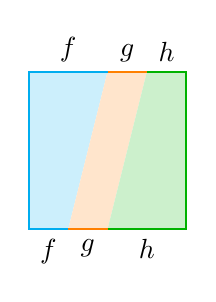
\begin{tikzpicture}
			\path [fill=cyan!20] (0,1)--(-1,1)--(-1,-1)--(-0.5,-1);
			\path [fill=orange!20] (0.5,1)--(0,1)--(-0.5,-1)--(0,-1);
			\path [fill=black!30!green!20] (0.5,1)--(0,-1)--(1,-1)--(1,1);

			\draw [color=cyan, thick] (-0.5,-1)
				-- node [color=black, pos=0.5, below]{$f$} (-1,-1) 
				-- (-1,1)
				-- node [color=black, pos=0.5, above]{$f$} (0,1);

			\draw [color=orange, thick] (-0.5,-1) 
				-- node [color=black, pos=0.5, below]{$g$} (0,-1);
			\draw [color=orange, thick] (0,1) 
				-- node [color=black, pos=0.5, above]{$g$} (0.5,1);

			\draw [color=black!30!green, thick] (0,-1) 
				-- node [color=black, pos=0.5, below]{$h$} (1,-1)
				-- (1,1)
				-- node [color=black, pos=0.5, above]{$h$} (0.5,1);		
		\end{tikzpicture}
	\end{center}
	We can check that $H(s,t)$ is a homotopy rel end points from $h\cdot(g\cdot f)$ to $(h\cdot g)\cdot f$.

	Define a path
	\begin{align*}
		c_x:[0,1] &\longrightarrow X\\
		s &\longmapsto x
	\end{align*}
	We can show that $c_x\cdot f\sim f$ and $f\cdot c_x\sim f$, which means $[c_x]$ is the identity of the group $\pi_1(X,x)$. 

	Given any $[f]\in \pi_1(X,x)$, it is easy to check $\left[f\right]^{-1}\in \pi_1(X,x)$ and $[f]^{-1}\cdot[f]=[f]\cdot[f]^{-1}=[c_x]$.
}

\dfn{Fundamental Groupoid}{
	Let $X$ be a topological space. Define $\Pi_1(X)$ to a category, where $\Obj(\Pi_1(X))=X$ and $\Hom_{\Pi_1(X)}(x,y)=\{[f]\mid f:[0,1]\to X \text{ is a path from $x$ to $y$}\}$. $\Pi_1(X)$ is a groupoid and called the fundamental groupoid of $X$.
}
\dfn{Fundamental Groupoid Functor}{
	Define $\Pi_1:\Top\to\Grpd$ as follows
	\[
	\begin{tikzcd}[ampersand replacement=\&]
		X  \arrow[dd, "f"{name=L, left}] 
		\&[-25pt] \& [+10pt] 
		\& [-30pt] \Pi_1(X) \arrow[dd, "f_*"{name=R}]\&[-30pt]\ni
		\&[-30pt]\left[\gamma\right]\arrow[dd,mapsto]\\ [-10pt] 
		\&  \phantom{.}\arrow[r, "\Pi_1", squigarrow]\&\phantom{.}  \&   \\[-10pt] 
		Y \& \& \& \Pi_1(Y)\&\ni\&\left[f\circ \gamma\right]
	\end{tikzcd}
	\]
}
\pf{
	First, we will show that $\Pi_1(f)$ is well-defined, namely for any two paths $\gamma_1$ and $\gamma_2$ in $X$,
	\[
		\gamma_1\sim \gamma_2 \implies [f\circ \gamma_1] = [f\circ \gamma_2].
	\]
	Suppose $\gamma_1\sim \gamma_2$ and $H$ is a homotopy rel end points from $\gamma_2$ to $\gamma_2$. Then $r(s,t):=f(H(s, t))$
	is a homotopy rel end points from $f\circ \gamma_1$ to $f\circ \gamma_2$, because for all $s\in[0,1]$,
	\begin{align*}
		r(s,0)&=f(H(s,0))=f(\gamma_1(s))=f\circ \gamma_1(s),\\
		r(s,1)&=f(H(s,1))=f(\gamma_2(s))=f\circ \gamma_2(s).
	\end{align*}
	Thus we have $f\circ \gamma_1\sim f\circ \gamma_2$, which implies $\Pi_1(f)$ is well-defined.
	To verify the functinality of $\Pi_1$, we have to show that
	\[
		(g\circ f)_* = g_*\circ f_*,
	\]
	or equivalently for all $[\gamma]\in \Pi_1(X)$,
	\[
		[(g\circ f)\circ \gamma]=[g\circ (f\circ \gamma)],
	\]
	which clearly holds. 
}
\dfn{Connected Groupoid}{
	A groupoid $\mathsf{G}$ is called \textbf{connected} if for any two objects $x,y$ of $\mathsf{G}$, $\Hom_{\mathsf{G}}(x,y)\ne \varnothing$.
}
\prop{Fundamental Groupoid of a Path-Connected Space is Connected}{
	Let $X$ be a topological space. Then $\Pi_1(X)$ is connected if and only if $X$ is path-connected.
}
\pf{
	$\Hom_{\Pi_1(X)}(x,y)\ne \varnothing$ if and only if there exists a path from $x$ to $y$.
}
\dfn{Simply Connected Space}{
	A topological space $X$ is called \textbf{simply connected} if it is path-connected and $\pi_1(X,x_0)$ is trivial for some $x_0\in X$.
}
\dfn{Locally Simply Connected Space}{
	A topological space $X$ is called \textbf{locally simply connected} if for every $x\in X$ there exists an open 
	neighborhood $U$ of $x$ such that $U$ is simply connected.
}
\dfn{Semi-locally Simply Connected Space}{
	A topological space $X$ is called \textbf{semi-locally simply connected} if for every $x\in X$ there exists an open neighborhood $U$ of $x$ with the property that every loop in $U$ can be contracted to a single point within $X$.

	Equivalently, $X$ is semi-locally simply connected if for every $x\in X$ there exists an open neighborhood $U$ of $x$ such that the inclusion map $i:U\to X$ induces the trivial homomorphism $i_*:\pi_1(U,x)\to \pi_1(X,x)$.
	
}
\prop{}{
	The following implications hold:
	\begin{itemize}
		\item simply connectedness $\implies$ semi-locally simply connected $+$ path-connected.
		\item locally simply connected $\implies$ semi-locally simply connected $+$ locally path-connected.
	\end{itemize}
}
\section{Homotopy Equivalence}
\dfn{Homotopy Equivalence}{
	Let $X$ and $Y$ be topological spaces. A continuous map $f:X\to Y$ is called a \textbf{homotopy equivalence} if there exists a continuous map $g:Y\to X$ such that $g\circ f\simeq \mathrm{id}_X$ and $f\circ g\simeq \mathrm{id}_Y$. In this case, we say $X$ and $Y$ are \textbf{homotopy equivalent} and write $X\simeq Y$.
}
\dfn{Deformation Retraction}{
	Let $X$ be a topological space and $A\subseteq X$. A \textbf{deformation retraction} of $X$ onto $A$ is a homotopy $H:X\times [0,1]\to X$ such that
	\begin{itemize}
		\item $H(x,0)=x$ for all $x\in X$;
		\item $H(x,1)\in A$ for all $x\in X$;
		\item $H(a,1)=a$ for all $a\in A$.
	\end{itemize}
}
\chapter{Covering spaces}
\section{Covering spaces}
\dfn{Category of Pointed Topological Spaces}{
	The \textbf{category of pointed topological spaces} $\Top_*$ is the coslice category $\left(\{*\}/\Top\right)$ defined explicitly as follows
	\begin{itemize}
		\item $\Obj(\Top_*)$ is the class of all pairs $(X,x)$, where $X$ is a topological space and $x\in X$;
		\item $\Hom_{\Top_*}((X,x),(Y,y))$ is the class of all continuous maps $f:X\to Y$ such that $f(x)=y$. 
	\end{itemize}
	Morphisms in $\Top_*$ are called \textbf{based maps}.
}
\dfn{Covering}{
	Let $X$ be a topological space. A \textbf{covering} of $X$ is a continuous map
$$
p: E \longrightarrow X
$$
such that there exists a discrete space $D$ and for every $x \in X$ an open neighborhood $U \subseteq X$, such that $p^{-1}(U)=\bigsqcup_{d \in D} V_d$ and $\left.p\right|_{V_d}: V_d \rightarrow U$ is a homeomorphism for every $d \in D$. Such open neighborhood $U$ is called a \textbf{fundamental neighborhood} for $x$. The open sets $V_d$ are called \textbf{sheets}.
}
A based map $p:(E,e)\to (X,x)$ is called a \textbf{covering map} if $p:E\to X$ is a covering. 

A covering space is a fiber bundle with discrete fiber $D$, illustrated as follows
\[\xymatrix{
			p^{-1}(U)\ar[rd]_{p}\ar[rr]^{\phi}  & &U\times D\ar[ld]^{p_1}\\
			&U&
			}\]
\prop{Covering Map is Local Homeomorphism}{
	The covering $p:E\to X$ is a local homeomorphism.
}
\dfn{Lifting}{
	Let $p:E\to X$ and $f:Y\to X$ be continuous maps. A lifting of $f$ along $p$ is a continuous map $\widetilde{f}:Y\to E$ such that the following diagram commutes
	\[\xymatrix{
			& E\ar[d]^{p}\\
			Y\ar[ur]^{\widetilde{f}}\ar[r]_{f} &X
			}\]
}
Throughout this chapter, we assume that all given spaces are connected and locally path
connected.

\lemm{}{
	Let $p: E \rightarrow X$ be a covering. Then the diagonal $D=\{(e, e) \in E \times E \mid e\in E\}$ is open and closed in $Z=\{(e_1, e_2) \in E \times E \mid p(e_1)=p(e_2)\}$.
}
\pf{
	Given any $(e,e)\in D$, suppose $U$ is a fundamental neighborhood of $p(e)$ and $V_e$ is the corresponding sheet such that $\left.p\right|_{V_e}:V_e\to U$ is a homeomorphism. Then for any $e_1,e_2\in V_e$, we have
	\[
		p(e_1)=p(e_2)\implies e_1=e_2,
	\]
	which implies $Z \cap\left(V_e \times V_e\right)=W_e$ is contained in $D$. Note $W_e$ is an open neighbourhood of $(e, e)$ in $Z$. We see $D$ is open in $Z$.

	Given any $(e_1,e_2)\in Z-D$, suppose $U$ is a fundamental neighborhood of $p(e_1)=p(e_2)$ and $V_{e_1}$ and $V_{e_2}$ are the sheets such that $\left.p\right|_{V_{e_1}}:V_{e_1}\to U$, $\left.p\right|_{V_{e_2}}:V_{e_2}\to U$ are a homeomorphisms. Since $e_1 \ne e_2$, we have $V_{e_1} \cap V_{e_2}=\varnothing$ and $\left(V_{e_1}\times V_{e_2}\right)\cap D=\varnothing$. Hence $Z \cap\left(V_{e_1} \times V_{e_2} \right)$  is contained in $Z-D$. Note that $Z \cap\left(V_{e_1} \times V_{e_2} \right)$ is an open neighbourhood of $(e_1,e_2)$ in $Z$. This shows that $Z- D$ is also open.
}

\prop{Uniqueness of Liftings}{
Let $p: E \rightarrow X$ be a covering and $f: Y \rightarrow X$ be a continuous map. Suppose $Y$ is connected. If $\widetilde{f}_1, \widetilde{f}_2: Y \rightarrow E$ be liftings of $f: Y \rightarrow X$ such that $\widetilde{f}_1(y_0)=\widetilde{f}_2(y_0)$ for some $y_0\in Y$, then $\widetilde{f}_1=\widetilde{f}_2$.
\[
	\begin{tikzcd}[ampersand replacement=\&]
		\{y_0\} \arrow[r, "\theta"] \arrow[d, "i_{y_0}"', hook]                      \& E \arrow[d, "p"] \\ [+8pt]
		Y \arrow[r, "f"'] \arrow[ru, "\widetilde{f}", dashed] \& X               
	\end{tikzcd}
	\]
	In other words, given that the outer square of the diagram commutes, if there exists a diagonal arrow $\widetilde{f}:Y\to E$ such that the whole diagram commutes, then $\widetilde{f}$ is unique.
}
\pf{
	Suppose $Z=\{(e_1, e_2) \in E \times E \mid p(e_1)=p(e_2)\}$ and $D=\{(e, e) \in E \times E \mid e\in E\}$. We can define a continuous map
	\begin{align*}
		g: Y &\longrightarrow Z\\
		y &\longmapsto \left(\widetilde{f}_1(y), \widetilde{f}_2(y)\right)
	\end{align*}
	 By assumption, $g(y_0)\in D$, which guarantees $g^{-1}(D)$ is nonempty. By lemma 4.1.1, we see $g^{-1}(D)$ is open and closed in $Y$. If $Y$ is connected, then $g^{-1}(D)=Y\implies g(Y)\subseteq D$. In other words, we have
	 \[
		\left\{\left(\widetilde{f}_1(y), \widetilde{f}_2(y)\right) \midv y \in Y\right\} \subseteq\{(e, e) \in E \times E \mid e\in E\}.
		\]
	Therefore, we show that	$\widetilde{f}_1=\widetilde{f}_2$.
}



\dfn{Homotopy Lifting Property}{
	Define the inclusion $\iota_0:Y\to Y\times I,y\mapsto(y,0)$, namely $\iota_0=\mathrm{id}\times c_0$. A map $p: E \rightarrow X$ has the \textbf{homotopy lifting property} for the space $Y$ if the following holds: 
	\begin{itemize}
		\item for each homotopy $f_\bullet: Y \times I \rightarrow X$, and
		\item for each map $\widetilde{f}_0: Y \rightarrow E$ that lifts $f_0:=f_{\bullet} \circ\iota_0$, i.e. satisfies $p \circ \widetilde{f}_0=f_{\bullet} \circ\iota_0=f_0$,
	\end{itemize}
	there exists a homotopy $\widetilde{f}_{\bullet}: Y \times I \rightarrow E$ with $p \circ \widetilde{f}_{\bullet}=f_{\bullet}$ and $ \widetilde{f}_{\bullet} \circ \iota_0=\widetilde{f}_0$. In other words, homotopy lifting property means that whenever the outer square of the following diagram commutes, there exists a diagonal arrow $\widetilde{f}_{\bullet}:Y\times I\to E$ such that the whole diagram commutes.
	\[
	\begin{tikzcd}[ampersand replacement=\&]
		Y \arrow[r, "\widetilde{f}_0"] \arrow[d, "\iota_0"', hook]                      \& E \arrow[d, "p"] \\ [+10pt]
		Y\times I \arrow[r, "f_\bullet"'] \arrow[ru, "\widetilde{f}_{\bullet}", dashed] \& X               
	\end{tikzcd}
	\]
	We call $\widetilde{f}_{\bullet}$ a lifting of $f_{\bullet}$ with initial condition $\widetilde{f}_0$. The map $p$ is called a \textbf{fibration} if it has the homotopy lifting property for all spaces.
}

\thm{Covering is Fibration}{
	A covering $p: E \rightarrow B$ is a fibration. Moreover, the homotopy lifting is unique.
}
\pf{
	First we can show homotopy lifting is unique if it exists. Suppose there exist two homotopies $\widetilde{f}_{\bullet}$ and $\widetilde{g}_{\bullet}$ either of which lifts $f_{\bullet}$ with initial condition $\widetilde{f}_0$. Then we have the following commutative diagram.
	\[
	\begin{tikzcd}[ampersand replacement=\&]
		\{y\}\arrow[r, "i_y", hook]\arrow[d, "\iota_0"', hook]\&Y \arrow[r, "\widetilde{f}_0"] \arrow[d, "\iota_0"', hook]                      \& E \arrow[d, "p"] \\ [+13pt]
		\{y\} \arrow[r, "i_y"', hook]  \times I\&Y\times I \arrow[r, "f_\bullet"'] \arrow[ru, "\widetilde{f}_{\bullet}", dashed] \& X               
	\end{tikzcd}
	\]
	Since $\{y\}\times I$ is connected, according to the uniqueness of liftings, we see $\widetilde{f}_{\bullet}\circ i_y=\widetilde{g}_{\bullet}\circ i_y$. Note that $y$ is arbitrary, we have $\widetilde{f}_{\bullet}=\widetilde{g}_{\bullet}$.
}

Taking $Y=\{*\}$ in the homotopy lifting property gives the following corollary.

\cor{Unique Path Lifting}{
	Let $p: (E,e) \to (X,x)$ be a covering. A path $\gamma: I \to X$ with $\gamma(0)=x$ lifts uniquely to a path $\widetilde{\gamma}: I \to E$ such that $\widetilde{\gamma}(0)=e$ and $p \circ \widetilde{\gamma}=\gamma$. We may use $\widetilde{\gamma}^e$ to denote this unique lifting if we want to emphasize the starting point $e$.
	\[
	\begin{tikzcd}[ampersand replacement=\&]
		\{*\} \arrow[r, "c_e"] \arrow[d, "c_0"', hook]                      \& E \arrow[d, "p"] \\ [+8pt]
		 I \arrow[r, "\gamma"'] \arrow[ru, "\widetilde{\gamma}", dashed] \& X               
	\end{tikzcd}
	\]
}
\pf{
	We can also prove it independently. Suppose $\mathcal{F}=\left\{U_\alpha\right\}_{\alpha\in A}$ is a collection of fundamental neighborhoods such that $\cup_{\alpha\in A}U_\alpha=X$. Let $f:I\to X$ be a path with $f(0)=x$. Then $\left\{f^{-1}(U_\alpha)\right\}_{\alpha\in A}$ is an open cover of $I$, so has a finite subcover $\left\{f^{-1}(U_{i})\right\}_{i=1}^m$. Let $0=t_0<t_1<\cdots<t_n=1$ be such that $f([t_{k-1},t_k])\subseteq U_{i_k}$ where $1\le i_k \le m$. \\
	We will construct a sequence of maps $\widetilde{f}_k:[t_{k-1},t_k]\to E$ by induction on $k$. Suppose $k=0$. Note that $f(0)=x\in U_{i_0}$ and there exists a homeomorphism $\left.p\right|_{V_0}: E\supseteq V_0\to U_{i_0}$ such that $\left.p\right|_{V_0}(e)=x$. We can define $\widetilde{f}_0=\left(\left.p\right|_{V_0}\right)^{-1}\circ f|_{[t_0,t_1]}$ and check that $\widetilde{f}_0$ is a lifting of $f|_{[t_0,t_1]}$ such that $\widetilde{f}_0(0)=e$. \\
	Suppose we have constructed $\widetilde{f}_0,\widetilde{f}_1,\cdots,\widetilde{f}_{k-1}$. Note that $f(t_{k})=p\left(\widetilde{f}_{k-1}(t_k)\right)\in U_{i_k}$ and there exists a homeomorphism $\left.p\right|_{V_k}: E\supseteq V_k\to U_{i_k}$ such that $\left.p\right|_{V_{k}}\left(\widetilde{f}_{k-1}(t_k)\right)=f(t_k)$. We can define $\widetilde{f}_k=\left(\left.p\right|_{V_k}\right)^{-1}\circ f|_{[t_k,t_{k+1}]}$ and check that $\widetilde{f}_k$ is a lifting of $f|_{[t_k,t_{k+1}]}$ such that $\widetilde{f}_k(t_{k})=\widetilde{f}_{k-1}(t_{k})$. \\
	By defining 
	\[
		\widetilde{f}(t)=\widetilde{f}_k(t)\text{ for }t_{k}\le t\le t_{k+1},	
	\]
	we can connect the sequence of maps $\widetilde{f}_k$ to get a path $\widetilde{f}:I\to E$ such that $\widetilde{f}(0)=e$ and $p\circ \widetilde{f}=f$. Since $I$ is connected, we know $\widetilde{f}$ is unique.
}

\prop[Lifting]{Lifting of Homotopic Paths}{
	\label{my_proposition}
	Let $p: (E,e) \to (X,x)$ be a covering. If $\gamma_0 \sim \gamma_1: I \to X$ are homotopic paths that both start from $x$, then the lifted paths $\widetilde{\gamma}_0, \widetilde{\gamma}_1: I \to E$ that both start at $e$ are also homotopic. Moreover, if $\gamma_0,\gamma_1$ have the same end point, then $\widetilde{\gamma}_0, \widetilde{\gamma}_1$ also have then same end point.\\
	Define 
	\begin{align*}
		\eta(s,t)=\begin{cases}
			e & \text{if }s=0\text{ and }0\le t\le 1 \\
			\widetilde{\gamma}_0(s) & \text{if }0\le s\le 1 \text{ and }t=0\\
			\widetilde{\gamma}_1(s) & \text{if }0\le s\le 1 \text{ and }t=1\\
		\end{cases}
	\end{align*}
	Given that the outer square of the following diagram commutes, there exists a unique diagonal arrow $\widetilde{\gamma}_\bullet:I\times I\to E$ such that the whole diagram commutes.
	\[
	\begin{tikzcd}[ampersand replacement=\&]
		 (\{0\}\times I )\cup (I\times\partial I ) \arrow[r, "\eta"] \arrow[d, "i"', hook]                      \& E \arrow[d, "p"] \\ [+20pt]
		I \times I \arrow[r, "\gamma_\bullet"'] \arrow[ru, "\widetilde{\gamma}_\bullet", dashed] \& X               
	\end{tikzcd}
	\]
}
\pf{
	We have the following diagram
	\[
	\begin{tikzcd}[ampersand replacement=\&]
		I \arrow[d, "\iota_0"', hook]\arrow[r, "g\circ\iota_0"]\&(\{0\}\times I )\cup (I\times\partial I ) \arrow[r, "\eta"] \arrow[d, "i"', hook]                      \& E \arrow[d, "p"] \\ [+22pt]
		I \times I\arrow[r, "g"']\&I \times I \arrow[r, "\gamma_\bullet"'] \arrow[ru, "\widetilde{\gamma}_\bullet", dashed] \& X               
	\end{tikzcd}
	\]
	where the two squares are commutative. The $(g\circ\iota_0, g)$ is an isomorphism from $\iota_0$ to $i$, which is illustrated as follows
	\begin{center}
		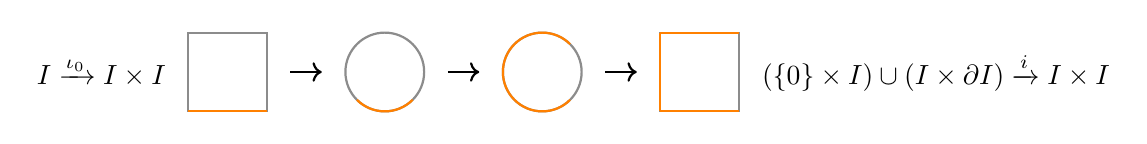
\begin{tikzpicture}
		% Draw the unit square with 90% gray line
		\draw[thick, black!45] (0,0) rectangle (1,1);
		% Draw the 3 specified lines with thick orange color
		\draw[thick, black!45] (0,0) -- (0,1); % {0} x I
		\draw[thick, orange] (0,0) -- (1,0); % I x {0}
		\draw[thick, black!45] (0,1) -- (1,1); % I x {1}

		% Draw a unit circle with radius 0.5
		\draw[thick, black!45] (2.5,0.5) circle (0.5);
		% Highlight 1/4 of the arc
		\draw[thick, orange] (2.5,0.5) ++(225:0.5) arc (225:315:0.5);

		% Draw a unit circle with radius 0.5
		\draw[thick, black!45] (4.5,0.5) circle (0.5);
		\draw[thick, orange] (4.5,0.5) ++(45:0.5) arc (45:315:0.5);

		% Second square
		\draw[thick, black!45] (6,0) rectangle (7,1); % fill the square with 90% grey
		\draw[thick, orange] (6,0) -- (6,1); % left vertical line
		\draw[thick, orange] (6,0) -- (7,0); % bottom horizontal line
		\draw[thick, orange] (6,1) -- (7,1); % top horizontal line

		% Arrow
		\draw[->, thick] (1.3,0.5) -- (1.7,0.5);
		\draw[->, thick] (3.3,0.5) -- (3.7,0.5);
		\draw[->, thick] (5.3,0.5) -- (5.7,0.5);

		% Labels
		\node at (-1.1,0.5) {$I\xrightarrow{\iota_0}I\times I$};
		\node at (9.5,0.5) {$(\{0\}\times I )\cup (I\times\partial I )\xrightarrow{i}I\times I$};
	\end{tikzpicture}
	\end{center}
	The homeomorphism $g$ maps the leftmost square to the rightmost square, and its restriction to $I\times\{0\}$ is also a homeomorphism which maps the orange line within the leftmost square to the orange line within the rightmost square.\\
	Suppose the unique homotopy lifting of $\gamma_{\bullet}\circ g$ is $h:I\times I \to E$, then we can take $\widetilde{\gamma}_\bullet=h\circ g^{-1}$ and check that it is a homotopy lifting of $\gamma_\bullet$ that makes the whole diagram commute. Suppose there exists another homotopy lifting $\widetilde{\gamma}_\bullet^\prime$ of $\gamma_\bullet$. Then by the uniqueness of $h$ we have $\widetilde{\gamma}_\bullet^\prime\circ g=\widetilde{\gamma}_\bullet\circ g=h$, which implies $\widetilde{\gamma}_\bullet^\prime=\widetilde{\gamma}_\bullet$.
}
\dfn{Star Set}{
	Let $\mathsf{C}$ be a category and $x$ is an object of $\mathsf{C}$. The \textbf{star set} of $x$ in $\mathsf{C}$ is defined as
	$\mathrm{St}(x)=\mathrm{Obj}\left(x/\mathsf{C}\right)$.
}
\dfn{Covering of Groupoid}{
	Let $\mathsf{E}$ and $\mathsf{B}$ be two groupoids. A functor $p:\mathsf{E}\to\mathsf{B}$ is a \textbf{covering of groupoid} if it is surjective on objects and for each object $e$ of $\mathsf{E}$ 
	\[
		p^{e}:\mathrm{St}(e)\to\mathrm{St}(p(e))
	\]
	is a bijection.
}

\prop[space_covering_induces_groupoid_covering]{Covering of Spaces Induces Covering of Groupoids}{
	If $p : E \to X$ is a covering of spaces, then $p_*: \Pi_1(E) \to \Pi_1(X)$ is a covering of groupoid.
}
\pf{
	This a corollary of \Cref{th:Lifting}. Suppose $p : E \to X$ is a covering of spaces and $e\in E$. Given a map $p_*^{e}:\mathrm{St}(e)\to\mathrm{St}(p(e))$, we can define
	\begin{align*}
		q^e:\mathrm{St}(p(e))&\to \mathrm{St}(e)\\
		[\gamma]&\mapsto [\widetilde{\gamma}^e]
	\end{align*}
	which is well-defined since homotopic paths with the same starting point lift to homotopic paths with the same starting point. Then we can check that
	\[
		p_*^{e}\circ q^e([\gamma])=p([\widetilde{\gamma}^e])=[p\circ\widetilde{\gamma}^e]=[\gamma]
	\]
	and
	\[
		q^e\circ p_*^{e}([\gamma])=q^e([p\circ\gamma])=\left[\left(\widetilde{p\circ\gamma}\right)^e\right]=[\gamma],
	\]
	where $\left(\widetilde{p\circ\gamma}\right)^e=\gamma$ holds since $\gamma$ is a lifting of $p\circ\gamma$ starting at $e$.
}

\cor[GroupEmbedding]{Fundamental Group Embedding for Covering Spaces}{
	Suppose $p: (E,e) \to (X,x)$ is a covering. Then $p_*: \pi_1(E, e) \to \pi_1(X, x)$ is a monomorphism. The image $p_*(\pi_1(E, e))$ consists of all equivalent classes of loops in $X$ that lift to loops in $E$ based at $e$.
}
\pf{ 
	According to \Cref{th:space_covering_induces_groupoid_covering}, $p^e:\mathrm{St}(e)\to\mathrm{St}(p(e))$ is a bijection. Note that $p_*: \pi_1(E, e) \to \pi_1(X, x)$ as a map between sets is the restriction of $p^e$ to $\pi_1(E, e)$. Therefore it is injective, which implies $p_*$ is a monomorphism between groups.
}
\prop{Change Basepoint in Fiber (Groupoid Version)}{
	Let $p:\mathsf{E}\to\mathsf{B}$ be a covering of groupoid with $\mathsf{E}$ being connected. Suppose $e_1,e_2$ are two objects of $\mathsf{E}$ such that $p(e_1)=p(e_2)=x$, then $p(\mathrm{Aut}_\mathsf{E}(e_1))$ and $p(\mathrm{Aut}_\mathsf{E}(e_2))$ are conjugate subgroups in $\mathrm{Aut}_{\mathsf{B}}(x)$. This gives a bijection between $p^{-1}(x)$ and the conjugacy class of the subgroup $p(\mathrm{Aut}_\mathsf{E}(e_1))$ in $\mathrm{Aut}_{\mathsf{B}}(x)$.
	\begin{align*}
		p^{-1}(x) &\longrightarrow \mathrm{Cl}(p(\mathrm{Aut}_\mathsf{E}(e_1)))\\
		e &\longmapsto p(\mathrm{Aut}_\mathsf{E}(e))
	\end{align*}
}
\pf{ 
	Since $\mathsf{E}$ is connected, there exists a arrow $\gamma$ in $\mathsf{E}$ from $e_1$ to $e_2$. Then we have a commutative diagram
	\begin{center}
		\[
		\begin{tikzcd}[ampersand replacement=\&]
			\mathrm{Aut}_\mathsf{E}(e_1) \arrow[r, "p"] \arrow[d, "\gamma\circ(-)\circ\gamma^{-1}"'] \& \mathrm{Aut}_\mathsf{B}(x) \arrow[d, "p(\gamma)\circ(-)\circ p(\gamma)^{-1}"] \\
			\mathrm{Aut}_\mathsf{E}(e_2) \arrow[r, "p"'] \& \mathrm{Aut}_\mathsf{B}(x) 
		\end{tikzcd}
		\]
	\end{center}
	This implies $ p(\gamma)p(\mathrm{Aut}_\mathsf{E}(e_1))p(\gamma)^{-1}\subseteq p(\mathrm{Aut}_\mathsf{E}(e_2))$.
	Similarly, we have a commutative diagram
	\begin{center}
		\[
		\begin{tikzcd}[ampersand replacement=\&]
			\mathrm{Aut}_\mathsf{E}(e_2) \arrow[r, "p"] \arrow[d, "\gamma^{-1}\circ(-)\circ\gamma"'] \& \mathrm{Aut}_\mathsf{B}(x) \arrow[d, "p(\gamma)^{-1}\circ(-)\circ p(\gamma)"] \\
			\mathrm{Aut}_\mathsf{E}(e_1) \arrow[r, "p"'] \& \mathrm{Aut}_\mathsf{B}(x) 
		\end{tikzcd}
		\]
	\end{center}
	This implies $ p(\gamma)^{-1}p(\mathrm{Aut}_\mathsf{E}(e_2))p(\gamma)\subseteq p(\mathrm{Aut}_\mathsf{E}(e_1))$. Therefore, we have  $ p(\gamma)p(\mathrm{Aut}_\mathsf{E}(e_1))p(\gamma)^{-1}= p(\mathrm{Aut}_\mathsf{E}(e_2))$. The bijective property is clear from $p$ is bijective on star sets.
}
\cor{Change Basepoint in Fiber}{
	Let $E$ be a path-connected topological space and $p:E\to X$ be a covering. Suppose $x\in X$ and $e_1,e_2\in p^{-1}(x)$. Then we have a bijection
	\begin{align*}
		p^{-1}(x) &\longrightarrow \mathrm{Cl}(p_*(\pi_1(E,e_1)))\\
		e &\longmapsto p_*(\pi_1(E,e))
	\end{align*}
	If $\gamma$ is a path in $E$ from $e_1$ to $e_2$, then 
	$$
	p_*([\gamma])p_*(\pi_1(E,e_1))p_*([\gamma])^{-1}=p_*(\pi_1(E,e_2)).
	$$
}


\dfn{Monodromy Action (Groupoid Version)}{
	Let $p:\mathsf{E}\to\mathsf{B}$ be a covering of groupoids. The \textbf{monodromy of the covering $p$} is a functor $\mathrm{Fib}_{\mathsf{E}}:\mathsf{B}\to\mathsf{Set}$ defined as follows
	\begin{equation*}
		\begin{tikzcd}[ampersand replacement=\&]
			\mathsf{B}\&[-25pt]\&[+10pt]\&[-30pt]\mathsf{Set}\&[-20pt]\&[-30pt] \\ [-15pt] 
			x  \arrow[dd, "{\gamma}"{left}] \& \&  \&  p^{-1}(x) \arrow[dd, "\mathrm{Fib}_\mathsf{E}({\gamma})"]\&\ni\& e\arrow[dd,mapsto]\\ [-10pt] 
											\&  \phantom{.}\arrow[r, "\mathrm{Fib}_E", squigarrow]\&\phantom{.}  \&   \\[-10pt] 
			y \& \& \& p^{-1}(y)\&\ni\& e'
		\end{tikzcd}
	\end{equation*}
	where $e'$ is the target of the morphism $(p^e)^{-1}(\gamma)\in\mathrm{St}(e)$.
}
If we restricts $\mathrm{Fib}_{\mathsf{E}}$ to one object $x\in\mathsf{B}$, then we get a group action $\mathrm{Aut}_{\mathsf{B}}(x)\to\mathrm{Aut}_{\mathsf{Set}}(p^{-1}(x))$, which can also be written as
\begin{align*}
	\mathrm{Aut}_{\mathsf{B}}(x)\times p^{-1}(x) &\longrightarrow p^{-1}(x)\\
	(\gamma, e) &\longmapsto \gamma\cdot e:=\mathrm{Fib}_{\mathsf{E}}(\gamma)(e)
\end{align*}
Given any $e\in p^{-1}(x)$, we have $\mathrm{Stab}_{\mathrm{Aut}_{\mathsf{B}}(x)}(e)=p(\mathrm{Aut}_{\mathsf{E}}(e))$ and the following $\mathrm{Aut}_{\mathsf{B}}(x)$-set isomorphism
\begin{align*}
	\mathrm{Aut}_{\mathsf{B}}(x)/p(\mathrm{Aut}_{\mathsf{E}}(e)) &\stackrel{\sim}{\longrightarrow} \mathrm{Aut}_{\mathsf{B}}(x)e\\
	\gamma\hspace{1pt}p(\mathrm{Aut}_{\mathsf{E}}(e)) &\longmapsto \gamma\cdot e
\end{align*}

\dfn{Monodromy Action}{
	Let $X$ be a topological space and $p:E\to X$ be a covering. The \textbf{monodromy of the covering $p$} is a functor $\mathrm{Fib}_E:\Pi_1(X)\to \mathsf{Set}$ defined as follows
	\begin{equation*}
		\begin{tikzcd}[ampersand replacement=\&]
			\Pi_1(X)\&[-25pt]\&[+10pt]\&[-30pt]\mathsf{Set}\&[-20pt]\&[-30pt] \\ [-15pt] 
			x  \arrow[dd, "{[\gamma]}"{left}] \& \&  \&  p^{-1}(x) \arrow[dd, "\mathrm{Fib}_E({[\gamma]})"]\&\ni\& e=\widetilde{\gamma}^e(0)\arrow[dd,mapsto]\\ [-10pt] 
											\&  \phantom{.}\arrow[r, "\mathrm{Fib}_E", squigarrow]\&\phantom{.}  \&   \\[-10pt] 
			y \& \& \& p^{-1}(y)\&\ni\& e'=\widetilde{\gamma}^e(1)
		\end{tikzcd}
	\end{equation*}
}
\pf
{
	Since equivalent paths lift to equivalent paths, $\mathrm{Fib}_E([\gamma])$ is a well-defined map independent of the choice of $\gamma$ in equivalence class $[\gamma]$. To show $\mathrm{Fib}_E$ is a functor, we need to check that $\mathrm{Fib}_E([\gamma\cdot\psi])=\mathrm{Fib}_E([\psi])\circ\mathrm{Fib}_E([\gamma])$. Since both $\widetilde{\gamma}^e\cdot\widetilde{\psi}^{\widetilde{\gamma}^e(1)}$ and $\widetilde{(\gamma\cdot\psi)}^e$ are liftings of $\gamma\cdot\psi$ starting at $e$, we have $\widetilde{\gamma}^e\cdot\widetilde{\psi}^{\widetilde{\gamma}^e(1)}=\widetilde{(\gamma\cdot\psi)}^e$. Then
	\begin{align*}
		\mathrm{Fib}_E([\gamma\cdot\psi])(e)&=\widetilde{(\gamma\cdot\psi)}^e(1)\\
		&=\widetilde{\psi}^{\widetilde{\gamma}^e(1)}(1)\\
		&=\mathrm{Fib}_E([\psi])(\widetilde{\gamma}^e(1))\\
		&=\mathrm{Fib}_E([\psi])\circ\mathrm{Fib}_E([\gamma])(e).
	\end{align*}
	let $[c_x]$ be the identity element in $\pi_1(X,x)$, then $\mathrm{Fib}_E([c_x])$ is the identity map on $p^{-1}(x)$, hence $\mathrm{Fib}_E$ is a functor.
}
Monodromy functor can be viewed as a permutation representations of $\Pi_1(X)$. Specially, $\pi_1(X, x)$ acts on the fiber $p^{-1}(x)$ and makes it a $\pi_1(X, x)$-set. 

\dfn{Category of Coverings of $X$}{
	Let $X$ be a topological space. The \textbf{category of coverings over $X$} is a category $\mathsf{Cov}_X$ defined as follows:
	\begin{itemize}
		\item The objects of $\mathsf{Cov}_X$ are all coverings of $X$.
		\item The morphisms of between $p_1:E_1\to X$ and $p_2:E_2\to X$ are all continuous maps $f:E_1\to E_2$ such that the following diagram commutes
		\begin{equation*}
			\begin{tikzcd}[ampersand replacement=\&]
				E_1 \arrow[rr, "f"] \arrow[rd, "p_1"'] \& \& E_2 \arrow[ld, "p_2"] \\ 
				\& X \&
			\end{tikzcd}
		\end{equation*}
	\end{itemize}
}

\dfn{Monodromy Functor $\mathrm{Fib}$}{
	\textbf{Monodromy functor} $\mathrm{Fib}$ is defined as follows
	\begin{equation*}
		\begin{tikzcd}[ampersand replacement=\&]
			\mathsf{Cov}_X\&[-25pt]\&[+10pt]\&[-30pt]\left[\Pi_1(X),\mathsf{Set}\right]\&[-30pt]\&[-30pt] \\ [-15pt] 
			E_1  \arrow[dd, "f"{left}] \& \&  \& \mathrm{Fib}_{E_1} \arrow[dd, "\;\mathrm{Fib}(f)",Rightarrow]\\ [-10pt] 
											\&  \phantom{.}\arrow[r, "\mathrm{Fib}", squigarrow]\&\phantom{.}  \&   \\[-10pt] 
			E_2 \& \& \& \mathrm{Fib}_{E_2} \&\& 
		\end{tikzcd}
	\end{equation*}
	where the natural transformation $\mathrm{Fib}(f)$ is defined as follows: 
	\begin{equation*}
		\begin{tikzcd}[ampersand replacement=\&]
				\Pi_1(X)     \& x \arrow[r, "{[\gamma]}"]                                                  \&[+25pt] y                           \\
							 \& p^{-1}_1(x) \arrow[dd, "\left.f\right|_{p_{\scalebox{0.5}{$1$}}^{\scalebox{0.5}{$-1$}}(x)}"'] \arrow[r, "{\mathrm{Fib}_{E_1}({[\gamma]})}"] \& p^{-1}_1(y) \arrow[dd, "\left.f\right|_{p_{\scalebox{0.5}{$1$}}^{\scalebox{0.5}{$-1$}}(y)}"] \\
				\mathsf{Set} \&                                                                            \&                             \\
							 \& p^{-1}_2(y) \arrow[r, "{\mathrm{Fib}_{E_2}({[\gamma]})}"]                  \& p^{-1}_2(x)                
				\end{tikzcd}
	\end{equation*}
}
\pf{
	We need to first check the $\mathrm{Fib}(f)$ is natural. Suppose $e_1\in E_1$ and $e_2=f(e_1)\in E_2$. We need to show that $\mathrm{Fib}_{E_2}([\gamma])(e_2)=f(\mathrm{Fib}_{E_1}([\gamma])(e_1))$, i.e. $\widetilde{\gamma}^{e_2}(1)=f\circ \widetilde{\gamma}^{e_1}(1)$. Note that $p_2\circ \left(f\circ  \widetilde{\gamma}^{e_1}\right)=p_1\circ  \widetilde{\gamma}^{e_1}=\gamma$ and $f\circ  \widetilde{\gamma}^{e_1}(0)=f(e_1)=e_2$. We see both $f\circ  \widetilde{\gamma}^{e_1}$ and $\widetilde{\gamma}^{e_2}$ are liftings of $\gamma$ starting at $e_2$. Hence they are equal and we get $\widetilde{\gamma}^{e_2}(1)=f\circ \widetilde{\gamma}^{e_1}(1)$.\\
	What left is to show that $\mathrm{Fib}$ is a functor. Suppose $f:E_1\to E_2$ and $g:E_2\to E_3$ are two morphisms in $\mathsf{Cov}_X$. Note $\mathrm{Fib}(f)$ is just a restriction of $f$, it clear to see $\mathrm{Fib}(g\circ f)=\mathrm{Fib}(g)\circ \mathrm{Fib}(f)$. Also, $\mathrm{Fib}([c_x])=\mathrm{id}_{p^{-1}(x)}$ for any $x\in X$. Hence $\mathrm{Fib}$ is a functor.
}
\prop{Fundamental Groupoid of Covering Space}{
Let $p:E \to X$ be a covering. Then $\Pi_1(E)$ is isomorphic to the Grothendieck construction of the monodromy functor $\mathrm{Fib}_E: \Pi_1(X) \rightarrow \mathsf{Set}$
$$
\Pi_1(E) \cong \int_{\Pi_1(X)} \operatorname{Fib}_E
$$

whose
\begin{itemize}
	\item objects are pairs $(x, \widetilde{x})$ consisting of a point $x \in X$ and en element $\widetilde{x} \in \operatorname{Fib}_E(x)=p^{-1}(x)$;
	\item morphisms between $(x, \widetilde{x})$ and $\left(y, \widetilde{y}\right)$ are morphisms $[\gamma]: x \rightarrow y$ in $\Pi_1(X)$ such that $\operatorname{Fib}_E([\gamma])(\widetilde{x})=\widetilde{y}$.
\end{itemize}
Here we view $\mathsf{Set}$ as a discrete category to obtain the Grothendieck construction of $\mathrm{Fib}_E: \Pi_1(X) \rightarrow \mathsf{Set}\to\mathsf{Cat}$. 
}
\pf{
	Define a functor $G:\Pi_1(E)\to \int_{\Pi_1(X)} \operatorname{Fib}_E$ as follows:
	\begin{equation*}
		\begin{tikzcd}[ampersand replacement=\&]
			\Pi_1(E)\&[-25pt]\&[+10pt]\&[-30pt]\int_{\Pi_1(X)} \operatorname{Fib}_E\&[-30pt]\&[-30pt] \\ [-15pt] 
			\widetilde{x}  \arrow[dd, "{[\widetilde{\gamma}]}"{left}] \& \&  \& \left(p(\widetilde{x}),\widetilde{x}\right) \arrow[dd, "{\left[p\,\circ\widetilde{\gamma}\right]}"]\\ [-10pt] 
											\&  \phantom{.}\arrow[r, "G", squigarrow]\&\phantom{.}  \&   \\[-10pt] 
											\widetilde{y} \& \& \& \left(p(\widetilde{y}),\widetilde{y}\right) \&\& 
		\end{tikzcd}
	\end{equation*}
	We can check $G([\gamma])$ is indeed a morphism because 
	\[
		\operatorname{Fib}_E(\left[p\circ\widetilde{\gamma}\right])(\widetilde{x})=\left(\widetilde{p\circ\widetilde{\gamma}}\right)^{\widetilde{x}}(1)=\widetilde{\gamma}^{\widetilde{x}}(1)=\widetilde{y}.
	\]
	And we can define another functor $F:\int_{\Pi_1(X)} \operatorname{Fib}_E\to \Pi_1(E)$ as follows:
	\begin{equation*}
		\begin{tikzcd}[ampersand replacement=\&]
			\int_{\Pi_1(X)} \operatorname{Fib}_E\&[-25pt]\&[+10pt]\&[-30pt]\Pi_1(E)\&[-30pt]\&[-30pt] \\ [-15pt] 
			\left(x,\widetilde{x}\right)  \arrow[dd, "{\left[{\gamma}\right]}"{left}] \& \&  \& \widetilde{x} \arrow[dd, "{[\widetilde{\gamma}^{\widetilde{x}}]}"]\\ [-10pt] 
											\&  \phantom{.}\arrow[r, "F", squigarrow]\&\phantom{.}  \&   \\[-10pt] 
											\left(y,\widetilde{y}\right) \& \& \& \widetilde{y} \&\& 
		\end{tikzcd}
	\end{equation*}
	We can check $F([\gamma])$ is indeed a morphism because
	\[
		\widetilde{\gamma}^{\widetilde{x}}(1)=\operatorname{Fib}_E([\gamma])(\widetilde{x})=\widetilde{y}.
	\]
	Now we can check $F\circ G=\mathrm{id}_{\Pi_1(E)}$ and $G\circ F=\mathrm{id}_{\int_{\Pi_1(X)} \operatorname{Fib}_E}$. Hence $G$ is an isomorphism.
}
\prop[connectedness_and_monodromy]{}{
	Let $X$ be a path-connected topological space and let $E \rightarrow X$ be a covering. Then
	\begin{itemize}
		\item $E$ is path-connected if and only if $\mathrm{Fib}_E$ is a transitive action.
		\item $E$ is simply connected if and only if $\mathrm{Fib}_E$ is a transitive and free action.
	\end{itemize}
}
\pf{$E$ is path-connected if and only if for any $e_1,e_2\in E$ there exists a path $\psi$ in $E$ such that $\psi(0)=e_1$ and $\psi(1)=e_2$. According to the isomorphism $\Pi_1(E) \cong \int_{\Pi_1(X)} \operatorname{Fib}_E$, we see this is equivalent to that for any $e_1,e_2\in E$ there exists a path $\gamma$ in $X$ from $p(e_1)$ to $p(e_2)$ which lfits to $\psi$. Again this is equivalent to that for any $e_1,e_2\in E$ there exists a path $\gamma$ in $X$ such that $\mathrm{Fib}_E([\gamma])(e_1)=e_2$, i.e $\mathrm{Fib}_E$ is a transitive action.

If $E$ is simply connected, then for any $e\in E$ we have $\pi(E,e)=[c_e]$ is trivial. Let $x=p(e)$. According to the isomorphism $\Pi_1(E) \cong \int_{\Pi_1(X)} \operatorname{Fib}_E$, we see this is equivalent to that $[c_x]$ is the unique loop in $\pi(X,x)$ which can lift to a loop in $E$ based at $e$. Therefore, $[c_x]$ is the only element in $\pi_1(X,x)$ such that $\mathrm{Fib}_E([c_x])(e)=e$. Hence $\mathrm{Fib}_E$ is a free action. The converse is similar.
}

\dfn{Reconstructing Functor $\mathrm{Rec}:\left[\Pi_1(X),\mathsf{Set}\right] \to\mathsf{Cov}_X$}{
	Let $X$ be a locally path-connected and semi-locally simply connected topological space and let $\rho:\Pi_1(X)\to \mathsf{Set}$ be a functor. We define a covering space $E(\rho)$ of $X$ as follows:
	\begin{itemize}
		\item The underlying set of $E(\rho)$ is $\coprod_{x\in X}\rho(x)=\left\{(x,e)\mid x\in X,e\in\rho(x)\right\}$.
		\item The topology on $E(\rho)$ is generated by the topological basis
		\[
			V_{U,x} = \left\{ \left(x,\rho([\gamma])(e) \right) \in E(\rho) \;\vert\; \gamma \,\text{is a path from}\, x \,\text{to}\, x'\in U ,\; e\in\rho(x)\right\},
		\]
		where $U\subseteq X$ is an path-connected open neighborhood of $x\in X$ such that $\pi_1(U,x) \to \pi_1(X,x)$ is trivial.
	\end{itemize}
	Then we can define 
	\begin{align*}
		p:E(\rho)&\longrightarrow X\\
		(x,\rho(e))&\longmapsto x.
	\end{align*}
	and check $p$ is actually a covering. The \textbf{reconstructing functor} $\mathrm{Rec}$ is defined as
	\begin{equation*}
		\begin{tikzcd}[ampersand replacement=\&]
			\left[\Pi_1(X),\mathsf{Set}\right] \&[-25pt]\&[+10pt]\&[-30pt]\mathsf{Cov}_X\&[-20pt]\&[-30pt] \\ [-15pt] 
			\rho_1  \arrow[dd, "f"{left}, Rightarrow] \& \&  \&  E(\rho_1)\arrow[dd, "\mathrm{Rec}(f)"]\&\ni\& (x,e)\arrow[dd,mapsto]\\ [-10pt] 
											\&  \phantom{.}\arrow[r, "\mathrm{Rec}", squigarrow]\&\phantom{.}  \&   \\[-10pt] 
			\rho_2 \& \& \& E(\rho_2)\&\ni\& (x, f_x(e))
		\end{tikzcd}
	\end{equation*}
}

\thm[fundamental_thm_covering_spaces]{Fundamental Theorem of Covering Spaces}{
	Let $X$ be a locally path-connected and semi-locally simply connected topological space. Then the operations on
	\begin{itemize}
		\item extracting the monodromy $\operatorname{Fib}_E$ of a covering space $E$ over $X$
		\item reconstructing a covering space from monodromy $\operatorname{Rec}(\rho)$
	\end{itemize}
	constitute an equivalence of categories
	\begin{equation*}
		\begin{tikzcd}[ampersand replacement=\&, row sep=tiny]
			\mathsf{Cov}_X \arrow[rr, shift left=0.75ex, "\operatorname{Fib}"] \& \& \left[\Pi_1(X),\mathsf{Set}\right] \arrow[ll, shift left=0.75ex, "\operatorname{Rec}"]
		\end{tikzcd}
	\end{equation*}
	between the category of covering spaces, and the category of permutation groupoid representations of the fundamental groupoid of $X$.
}

\lemm{}{
	Let $p:E\to X$ be a covering. Let $\psi_1$ and $\psi_2$ be paths in $E$ beginning in $e$ and $\gamma_1=p\circ \psi_1$ and $\gamma_2=p\circ \psi_2$ be their projections to $X$. Then $\psi_1(1)=\psi_2(1)$ if and only if $\gamma_1(1)=\gamma_2(1)$ and $\left[\gamma_1 \cdot \gamma_2^{-}\right]\in p_* \left(\pi_1(E, e)\right)$.
}
\pf{
	If $\psi_1(1)=\psi_2(1)$, then $p_*\left(\left[\psi_1 \cdot \psi_2^{-}\right]\right)=\left[p_*(\psi_1) \cdot p_*(\psi_2^{-})\right]=\left[\gamma_1 \cdot \gamma_2^{-}\right]$. Conversely, by \Cref{th:GroupEmbedding}, we can lift the loop $\gamma_1 \cdot \gamma_2^{-}$ to a loop $\xi$ in $E$ based at $e$. Since for any $t\in [0,1]$,
	\[
	p\circ\xi\left(\frac{1}{2}t\right)=\gamma_1 \cdot \gamma_2^{-}\left(\frac{1}{2}t\right)=\gamma_1(t),
	\]
	we see both $\xi\left(\frac{1}{2}t\right)$ and $\psi_1(t)$ are liftings of $\gamma_1$ starting from $e$, which implies $\xi(\frac{1}{2})=\psi_1(1)$. Note $\xi^{-}$ is a lift of $\left(\gamma_1 \cdot \gamma_2^{-}\right)^{-}=\gamma_2 \cdot \gamma_1^{-}$. For any $t\in [0,1]$, we have
	\[
    p\circ \xi^{-}\left(\frac{1}{2}t\right)=\gamma_2 \cdot \gamma_1^{-}\left(\frac{1}{2}t\right)=\gamma_2(t).
	\]
	Therefore, both $\xi^{-}\left(\frac{1}{2}t\right)$ and $\psi_2(t)$ are liftings of $\gamma_2$ originating from $e$, which implies $\xi^{-}\left(\frac{1}{2}\right)=\psi_2(1)$. Since $\xi\left(\frac{1}{2}\right)=\xi^{-}\left(\frac{1}{2}\right)$, this demonstrates that $\psi_1(1)=\psi_2(1)$.
}

\prop[lifting_criterion]{Lifting Criterion}{
	Given a covering $p:\left(E, e\right) \rightarrow\left(X, x\right)$ and a map $f:\left(Y, y\right) \rightarrow\left(X, x\right)$ with $Y$ connected and locally path-connected, a lift $\widetilde{f}:\left(Y, y\right) \rightarrow\left(E, e\right)$ of $f$ exists iff $f_*\left(\pi_1\left(Y, y\right)\right) \subseteq p_*\left(\pi_1\left(E, e\right)\right)$.
}
\pf{ 
	First note that $Y$ is path-connected because $Y$ is both connected and locally path-connected. If such lift $\widetilde{f}$ exists, then for any $f_*([\gamma])\in f_*\left(\pi_1\left(Y, y\right)\right)$, we have $$f_*([\gamma])=[f\circ\gamma]=[p\circ\widetilde{f}\circ\gamma]=p_*\left(\widetilde{f}_*([\gamma])\right)=p_*\left(\left[\widetilde{f}\circ\gamma\right]\right)\in p_*\left(\pi_1(E,e)\right),$$
	which implies $f_*\left(\pi_1\left(Y, y\right)\right) \subseteq p_*\left(\pi_1\left(E, e\right)\right)$.
}

\prop[uniqueness_simply_connected_covering]{Uniqueness of Simply Connected Covering}{
	If $X$ is a connected and locally path-connected topological space and $p_1:E_1\to X$ and $p_2:E_2\to X$ be two simply connected coverings, then $p_1$ and $p_2$ are isomorphic coverings.
}
\pf{
	Let $p_1:E_1\to X$ and $p_2:E_2\to X$ be two simply connected coverings. Since $X$ is locally path-connected and $p_1,p_2$ are locally homeomorphisms, $E_1$ and $E_2$ are also locally path-connected. Suppose $p(e_1)=p(e_2)=x$ for some $e_1\in E_1$ and $e_2\in E_2$. Note $p_{1\,*}(\pi(E_1,e_1))=\{1_{\pi(X,x)}\}$. By \Cref{th:lifting_criterion}, there exists $f:(E_1,e_1)\to (E_2,e_2)$ such that $p_2\circ f=p_1$. Similarly, there exists $g:(E_2,e_2)\to (E_1,e_1)$ such that $p_1\circ g=p_2$. Since $p_1\circ (g\circ f)=p_2\circ f=p_1$ and $g\circ f(e_1)=e_1$, the uniqueness of lift guarantees $g\circ f=1_{E_1}$. Similarly we can show $f\circ g=1_{E_2}$. Therefore, $f$ is an isomorphism between $p_1$ and $p_2$.
}
\dfn{Universal Covering of Groupoids}{
	Let $p:\mathsf{E}\to \mathsf{B}$ be a covering of groupoids with $\mathsf{E}$, $\mathsf{B}$ being connected. $p$ is called a \textbf{universal covering of $\mathsf{B}$} if one of the following equivalent conditions holds:
	\begin{itemize}
		\item $p(\mathrm{Aut}_{\mathsf{E}}(e))$ is trivial
		\item $\mathrm{Aut}_{\mathsf{B}}(x)$ acts freely on $p^{-1}(x)$
	\end{itemize}
}
\prop{}{
	If $p:\mathsf{E}\to \mathsf{B}$ is a universal covering of connected groupoids, then for any $x\in \mathsf{B}$, we have the following $\mathrm{Aut}_{\mathsf{B}}(x)$-set isomorphism: 
	\begin{align*}
		\mathrm{Aut}_{\mathsf{B}}(x) &\stackrel{\sim}{\longrightarrow} p^{-1}(x)\\
		\gamma &\longmapsto \gamma\cdot e
	\end{align*}
}
\section{Universal Covering}
\dfn{Universal Covering}{
	Let $X$ be a topological space which is connected and locally path-connected. If $p: E \rightarrow X$ is a simply connected covering, then it is called a \textbf{universal covering} of $X$. If the universal covering of $X$ exists, it must be unique up to isomorphism.
}
\prop{Existence of Universal Covering}{
	If $X$ is a topological space which is connected, locally path-connected and semi-locally simply connected, then the universal covering of $X$ exists.
}
\pf{
	By \Cref{th:connectedness_and_monodromy} and \Cref{th:fundamental_thm_covering_spaces}, it is sufficient to show there exists a transitive and free representation of $\Pi_1(X)$. In fact, for any $x\in X$, the Hom functor $\mathrm{Hom}_{\Pi_1(X)}(x,-)$ is such a representation, which can be described as follows
	\begin{equation*}
		\begin{tikzcd}[ampersand replacement=\&]
			\Pi_1(X)\&[-25pt]\&[+20pt]\&[-20pt]\mathsf{Set}\&[-20pt]\&[-30pt] \\ [-15pt] 
			y_1  \arrow[dd, "{[\gamma]}"{left}] \& \&  \&  \mathrm{Hom}(x, y_1) \arrow[dd, "{[\gamma]_*}"]\&\ni\& {[\psi_1]}\arrow[dd,mapsto]\\ [-10pt] 
											\&  \phantom{.}\arrow[r, "{\mathrm{Hom}(x{,} -)}", squigarrow]\&\phantom{.}  \&   \\[-10pt] 
			y_2 \& \& \& \mathrm{Hom}(x, y_2)\&\ni\& {[\psi_1\cdot\gamma]}
		\end{tikzcd}
	\end{equation*}
	The fundamental group $\pi_1(y,X)$ acts on $\mathrm{Hom}(x,y)$ by
	\[
	[\gamma]*[\psi]=[\psi\cdot \gamma].	
	\]
	For any $[\psi_1],[\psi_2]\in\mathrm{Hom}(x,y)$, there exists a loop $[\xi]=[\psi_1^{-}\cdot\psi_2]\in \pi_1(y,X)$ such that $[\xi]*[\psi_1]=[\psi_2]$. Therefore, the action is transitive. 
	
	Given $[\gamma]\in\pi_1(y,X)$, if $[\gamma]*[\psi]=[\psi]$, then $[\psi\cdot\gamma]=[\psi]$, which implies $[\gamma]=[\psi^{-}]\cdot[\psi\cdot\gamma]=[\psi^{-}]\cdot[\psi]=[c_y]$. Therefore, the action is free.
}

\dfn{Normal Covering of Groupoids}{
	Let $p:\mathsf{E}\to \mathsf{B}$ be a covering of groupoids with $\mathsf{E}$, $\mathsf{B}$ being connected. If $p(\mathrm{Aut}_{\mathsf{E}}(e))\lhd \mathrm{Aut}_{\mathsf{B}}(p(e))$, then $p$ is called a \textbf{normal covering of $p$}.
}
\dfn{Normal Covering}{
	A covering $p: E \rightarrow X$ is called \textbf{normal} if for each $x \in X$ and any $e_1,e_2\in p^{-1}(x)$, there exists an isomorphism $\phi\in \mathrm{Aut}_{\mathsf{Cov}_X}(p)$ such that $\phi(e_1)=e_2$.
}
\prop{}{
	Let $p:\left(E, e\right) \rightarrow\left(X, x\right)$ where $E$ is path-connected and $X$ is path-connected and locally path-connected. Let $H=p_*\left(\pi_1\left(E,e\right)\right) \subseteq \pi_1\left(X, x\right)$. Then
	\begin{enumerate}[(i)]
		\item This covering $p$ is normal if and only if $H\lhd\pi_1\left(X, x_0\right)$.
		\item  $\mathrm{Aut}_{\mathsf{Cov}_X}(p)\cong\mathrm{N}_{\pi_1\left(X, x_0\right)}(H) / H$.
In particular, if $p$ is a normal covering, $\mathrm{Aut}_{\mathsf{Cov}_X}(p)\cong \pi_1\left(X, x_0\right) / H$. If $p$ is a universal covering, we have $G(\tilde{X}) \cong \pi_1(X)$.
	\end{enumerate}
}
\dfn{Continuous Group Action}{
	A \textbf{continuous group action} on a topological space $X$ is a group homomorphism $\phi:G\to \mathrm{Aut}_{\mathsf{Top}}(X)$, where $\mathrm{Aut}_{\mathsf{Top}}(X)$ is the group of homeomorphisms of $X$.
}

\dfn{Even Action}{
Let $G$ be a group acting continuously on a topological space $E$. The action of $E$ is \textbf{even} if each point $y \in Y$ has some neighborhood $U$ such that $gU\cap U=\varnothing$ for all $g\in G-\{1_G\}$.
}
\prop{}{
	If an action of a group $G$ on a space $E$ is even, then:
	\begin{enumerate}[(i)]
		\item The quotient map $p: E \rightarrow E / G$ is a normal covering.
		\item If $E$ is path-connected, then $G$ is the group of deck transformations of the covering $p:E \rightarrow E / G$ .
		\item If $E$ is path-connected and locally pathconnected, then $G$ is isomorphic to $\pi_1(E / G) / p_*\left(\pi_1(E)\right)$ 
	\end{enumerate}
}
\prop{}{
	For any continuous action of a topological group $G$ on a topological space $E$, the quotient map $p: E \rightarrow E / G$ is an open map.
}
\pf{
	For any $g \in G$ and any subset $U \subseteq M$, we define a set $g \cdot U \subseteq M$ by
$$
g \cdot U=\{g \cdot x: x \in U\} .
$$
If $U \subseteq M$ is open, then $\pi^{-1}(\pi(U))$ is equal to the union of all sets of the form $g \cdot U$ as $g$ ranges over $G$. Since $p \mapsto g \cdot p$ is a homeomorphism, each such set is open, and therefore $\pi^{-1}(\pi(U))$ is open in $M$. Becaues $\pi$ is a quotient map, this implies that $\pi(U)$ is open in $M / G$, and therefore $\pi$ is an open map.
}

\prop{}{
	Let $p: E \to X$ be a covering, let $x \in X$, and let $e, e^{\prime}$ be any two points in $p^{-1}(x)$.
	\begin{enumerate}[(i)]
		\item $p_*\left(\pi_1\left(E, e^{\prime}\right)\right)$ is conjugate to $p_*\left(\pi_1(E, e)\right)$.
		\item As $e'$ runs through $F_b$, the groups $p_*\left(\pi_1\left(E, e^{\prime}\right)\right)$ run through all conjugates of $p_*\left(\pi_1(E, e)\right)$ in $\pi_1(B, b)$.
	\end{enumerate}
}
\pf{
	
}
\chapter{Homology}
\section{Simplicial homology}

\dfn{Geometrically Independent}{
	Let $\left\{a_0, a_1, \cdots, a_k\right\}$ be points in $\mathbb{R}^n$. This set is said to be \textbf{geometrically independent} if the vectors
$$
a_1-a_0, \quad a_2-a_0, \quad \cdots, \quad a_k-a_0
$$
are linearly independent (as in linear algebra).
}

\dfn{Simplex}{
Let $\left\{a_0, a_1, \ldots, a_k\right\}$ be a geometrically independent set in $\mathbb{R}^n$. A $\textbf{$k$-simplex } \sigma$ spanned by these points is defined by
$$
\left\{x\in \mathbb{R}^n\;\left|\; x=\sum_{i=0}^k t_i a_i,\;\sum_{i=0}^k t_i=1,\;t_i \geq 0\text{ for }i = 0,1,\cdots, k\right.\right\}.
$$
}

\noindent A $k$-simplex spanned by $a_0, a_1, \ldots, a_k$ is the convex hull of these points.
\dfn{}{
Let $\sigma$ be a $k$-simplex spanned by $\left\{a_0, a_1, \ldots, a_k\right\}$.
\begin{enumerate}[(i)] 
	\item The points $a_0, a_1, \ldots, a_k$ are called the \textbf{vertices} of $\sigma$.
	\item The number $k$ is the \textbf{dimension} of $\sigma$.
	\item Any simplex spanned by a subset of $\left\{a_0, a_1, \cdots, a_k\right\}$ is called a \textbf{face} of $\sigma$. 
	\item The face spanned by $\left\{a_0, a_1, \cdots, a_k\right\}-\left\{a_i\right\}$ for some $i$ is called the \textbf{face opposite} to $a_i$.
	\item A face of $\sigma$ is called a \textbf{proper face} if it is not equal to $\sigma$.
	\item The union of all proper faces of $\sigma$ is called the \textbf{boundary} of $\sigma$, denoted by $\partial \sigma$.
	\item $\sigma-\partial \sigma$ is called the \textbf{interior} of $\sigma$.
\end{enumerate}
}
\dfn{Simplicial Complex}{
A \textbf{simplicial complex} $K$ is a collection of simplices in $\mathbb{R}^n$ (of possibly varying dimensions) such that
\begin{enumerate}[(i)] 
	\item Any face of a simplex in $K$ is also in $K$.
	\item The intersection of any two simplices in $K$ is a face of each of the two simplices, whenever the the intersection is non-empty.
\end{enumerate}
}

\dfn{Subcomplex}{
Let $K$ be a simplicial complex. If $L\subseteq K$ and $L$ is a simplicial complex, then $L$ is called a \textbf{subcomplex} of $K$.
}

\dfn{$p$-Skeleton}{
Given a simplicial complex $K$, the collection of all simplices of $K$ of dimension at $\operatorname{most} p$ is called the $\textbf{$p$-skeleton}$ of $K$ and is denoted $K^{(p)}$.
}
For example, $K^{(0)}$ is the set of vertices of $K$. $K^{(p)}$ is a subcomplex of $K$.

\dfn{Dimension Of A Simplicial Complex}{
If there exists an integer $N$ such that
$$
K^{(N-1)} \neq K \quad \text { and } \quad K^{(p)}=K \text { for }p\ge N ,
$$
then $K$ is said to have \textbf{dimension} $N$. Otherwise it is said to have infinite dimension.
}
\dfn{Finite Simplicial Complex}{
A simplicial complex $K$ is said to be \textbf{finite} if $K^{(0)}$ is finite.
}

\dfn{Realization Of A Simplicial Complex}{
The realization of a simplicial complex $K$ is a topological space $(|K|, \tau)$ such that
\begin{enumerate}[(i)] 
	\item $|K|$ is the union of all simplices in $K$, that is $|K|=\bigcup_{\sigma\in K}\sigma$.
	\item $F\subseteq |K|$ is a closed set in $(|K|, \tau)\iff$ for all simplices $\sigma\in K$, $F\cap \sigma$ is a closed set in $(\sigma,\nu_\sigma)$, where $\nu_\sigma$ is the subspace topology of Euclidean topology.
\end{enumerate}
}
For finite simplicial complexes $K$ with finite dimension, the topology $\tau$ coincides with the subspace topology of Euclidean topology. 
\dfn{Triangulation}{
	A \textbf{triangulation} of a topological space $X$ is a simplicial complex $K$ together with a homeomorphism $\phi:|K|\to X$.
}
All smooth manifolds are triangulable. For example, torus admits the following triangulation:
\begin{center}
	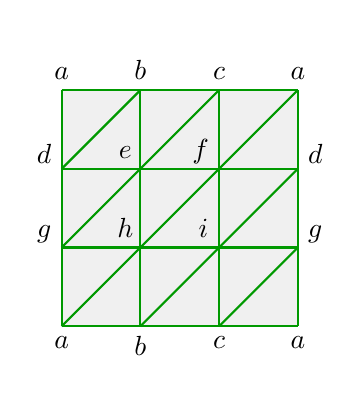
\begin{tikzpicture}[add_padding, x=1.5cm,y=1.5cm]
		\fill[fill=gray!12] (-1,-1)--(1,-1)--(1,1)--(-1,1)-- cycle;
		\draw [color=black!40!green,thick] (-1,-1) --
		node [color=black,pos=0,below]{$a$}
		node [color=black,pos=1/3,below]{$b$}
		node [color=black,pos=2/3,below]{$c$}
		node [color=black,pos=1,below]{$a$}(1,-1);
		\draw [color=black!40!green,thick] (-1,1/3)--		
		node [color=black,pos=0.27,above]{$e$} 
		 (1,1/3);
		\draw [color=black!40!green,thick] (-1,-1/3)--
		node [color=black,pos=0.27,above]{$h$} 
		node [color=black,pos=0.60,above]{$i$} (1,-1/3);
		\draw [color=black!40!green,thick] (-1/3,-1)--(-1/3,1);
		\draw [color=black!40!green,thick] (1/3,-1)--node [color=black,pos=0.74,left]{$f$}(1/3,1);
		\draw [color=black!40!green,thick] (1/3,-1)--(1,-1/3);
		\draw [color=black!40!green,thick] (-1/3,-1)--(1,1/3);
		\draw [color=black!40!green,thick] (-1,-1)--(1,1);
		\draw [color=black!40!green,thick] (-1,-1/3)--(1/3,1);
		\draw [color=black!40!green,thick] (-1,1/3)--(-1/3,1);
		\draw [color=black!40!green,thick] (-1,1)--
		node [color=black,pos=0.27,left]{$d$} 
		node [color=black,pos=0.61,left]{$g$} (-1,-1);
		\draw [color=black!40!green,thick] (1,1)--
		node [color=black,pos=0.27,right]{$d$} 
		node [color=black,pos=0.61,right]{$g$} (1,-1);
		\draw [color=black!40!green,thick] (-1,1)-- 
		node [color=black,pos=0,above]{$a$} 
		node [color=black,pos=1/3,above]{$b$} 
		node [color=black,pos=2/3,above]{$c$}
		node [color=black,pos=1,above]{$a$} 
		(1,1);
	\end{tikzpicture}
\end{center}

\dfn{Orientation Of Simplex}{
	Suppose $\sigma$ is a $k$-simplex spanned by $\left\{a_0, a_1, \ldots, a_k\right\}$. Let $V_{\sigma}$ to be the set of all ordered $k+1$-tuples of vertices of $\sigma$:
	\begin{align*}
		V_{\sigma}=\left\{\left(a_{s(0)},a_{s(1)},\cdots,a_{s(k)}\right)\mid s\in \mathrm{Sym}\left(\left\{0,1,\cdots,k\right\}\right)\right\}.
	\end{align*}
	Then $\sim$ is an equivalence relation on $V_{\sigma}$, where $\sim$ is defined by
	\begin{align*}
		\left(a_{s(0)},\cdots,a_{s(k)}\right)\sim\left(a_{s'(0)},\cdots,a_{s'(k)}\right)\iff \mathrm{sgn}(s)=\mathrm{sgn}(s').
	\end{align*}
	An orientation of $\sigma$ is a equivalence class of $V_{\sigma}/\sim$, denoted by
	\begin{align*}
		\left[a_{s(0)},a_{s(1)},\cdots,a_{s(k)}\right].
	\end{align*}
}
Every $k$-simplex has exactly $2$ orientations.
\dfn{Oriented Simplex}{
	Let $\sigma$ be a $k$-simplex spanned by $\left\{a_0, a_1, \ldots, a_k\right\}$. An \textbf{oriented $k$-simplex} is a pair $\left(\sigma, \left[a_{s(0)},a_{s(1)},\cdots,a_{s(k)}\right]\right)$, where $\sigma$ is a $k$-simplex and $\left[a_{s(0)},a_{s(1)},\cdots,a_{s(k)}\right]$ is an orientation of $\sigma$. The oriented $k$-simplex can be denoted by $\left\langle a_{s(0)},a_{s(1)},\cdots,a_{s(k)}\right\rangle$.
}

\dfn{Simplicial Chain Group}{
	Let $K$ be a simplicial complex and $F(K)$ be the free abelian group generated by all the oriented $k$-simplices in $K$. The $k$\textbf{-chain group} of $K$, denoted by $C_k(K)$, is defined as $F(K)$ modulo the relations
	\begin{align*}
		\left\langle a_{0}, \cdots ,a_{i},\cdots,a_{j},\cdots a_{k}\right\rangle=-\left\langle a_{0},\cdots ,a_{j},\cdots,a_{i},\cdots,a_{k}\right\rangle.
	\end{align*}
}
$C_k(K)$ is a free abelian group.
\dfn{Boundary Homomorphism}{
	Given a simplicial complex $K$, we can define the boundary homomorphism $\partial_k:C_k(K)\rightarrow C_{k-1}(K)$ on the basis of $C_k(K)$ by
	\begin{align*}
		\partial_k\left\langle a_{0},a_{1},\cdots,a_{k}\right\rangle=\sum_{i=0}^k(-1)^{i}\left\langle a_{0},a_{1},\cdots,a_{i-1},a_{i+1},\cdots,a_{k}\right\rangle,
	\end{align*}
	and then extend it to the whole $C_k(K)$ linearly.
}

\dfn{Cycle Group}{
	Let $K$ be a simplicial complex. The $k$-cycle group of $K$, denoted by $Z_k(K)$,  is defined as $\ker\partial_k$.
}

\dfn{Boundary Group}{
	Let $K$ be a simplicial complex. The $k$-boundary group of $K$, denoted by $B_k(K)$, is defined as $\mathrm{im}\,\partial_{k+1}$.
}

\prop{Chain Complex}{
	Let $K$ be a simplicial complex. Then we have $\partial_k\circ\partial_{k+1}=0$ or equivalently $B_k(K)\subseteq Z_k(K)$. Therefore we have a chain complex 
	\begin{align*}
		\cdots\stackrel{\partial_{k+2}}{\longrightarrow}  C_{k+1}(K)\stackrel{\partial_{k+1}}{\longrightarrow} C_{k}(K)\stackrel{\partial_{k}}{\longrightarrow} \cdots\stackrel{\partial_{2}}{\longrightarrow}  C_1(K)\stackrel{\partial_{1}}{\longrightarrow} C_0(K)\stackrel{\partial_{0}}{\longrightarrow}  0
	\end{align*}
	in $\mathsf{Ch}(\mathsf{Ab})$. 
}

\dfn{Simplical Homology Group}{
	For a simplicial complex $K$, the $k$-th homology group, $H_k(K)$ is defined to be the quotient group $Z_k(K) / B_k(K)$. An element of $H_k(K)$ is called a $k$-dimensional homology class of $K$. We say cycles $z_1, z_2\in Z_k(K)$ are homologous, written as $z_1\sim z_2$, if $z_1-z_2 \in B_k(K)$. 
}

\section{Singular homology}
\dfn{Standard Simplex}{
	For $n \geq 0$, the \textbf{standard $n$-simplex} $\Delta^n$ is the set $\Delta^n \subseteq \mathbb{R}^{n+1}$ defined by
$$
\Delta^n=\left\{\left(t_0, \cdots, t_n\right) \in \mathbb{R}^{n+1}\,\middle\vert\, \sum_{i=0}^n t_i=1, t_i \geq 0 \text { for all } i\right\} .
$$
Assume that $(e_0,\cdots,e_n)$ is the standand orthonormal basis of $\mathbb{R}^{n+1}$. Another way to describe $\Delta^n$ is to say that it is the $n$-simplex with vertices $\{e_0,\cdots,e_n\}$.
}
\dfn{Singular Simplex}{
	Let $X$ be a topological space. A \textbf{singular $n$-simplex} in $X$ is a continuous map $\sigma: \Delta^n \rightarrow X$. All the singular simplices in $X$ constitute $\mathrm{Hom}_{\mathsf{Top}}\left(\Delta^n, X\right)$.
}
\dfn{Singular Chain Group Functor $C_k$}{
	Given a topological space $X$, the \textbf{singular $k$-chain group} $C_k(X)$ of $X$ is the free abelian group generated by the singular simplices in $X$. \\
	The singular chain group functor $C_k:\mathsf{Top}\to\mathsf{Ab}$ can be defined as the composition of hom functor and free functor
	\begin{align*}
		\mathsf{Top}\xrightarrow{\mathrm{Hom}_{\mathsf{Top}}\left(\Delta^k, -\right)} \mathsf{Set}\xrightarrow{\mathbb{Z}^\oplus} \mathsf{Ab}
	\end{align*}
	We can also write it explicily as
	\begin{equation*}
		\begin{tikzcd}[ampersand replacement=\&]
			X  \arrow[dd, "f"{name=L, left}] \&[-25pt] \& [+10pt] \& [-30pt] C_k(X) \arrow[dd, "f_\sharp"{name=R}]\&[-30pt]\ni\&[-30pt]\sigma\arrow[dd,mapsto]\\ [-10pt] 
			                                \&  \phantom{.}\arrow[r, "C_k", squigarrow]\&\phantom{.}  \&   \\[-10pt] 
			Y \& \& \& C_k(Y)\&\ni\&f\circ \sigma
		\end{tikzcd}
	\end{equation*}
}

\dfn{Face Inclusion}{
	For any $k\ge 0$, we can define the \textbf{$i$-th face inclusion} by
	\begin{align*}
		l_i: \Delta^{k} &\longrightarrow  \Delta^{k+1}\\
		(t_0, \cdots, t_k) &\longmapsto (t_0, \cdots, t_{i-1}, 0, t_{i}, \cdots, t_{k})
	\end{align*}
	for $0\leq i\leq k+1$. 
}
Suppose $\{e_0,\cdots,e_{k+1}\}$ is the vertices of $\Delta^{k+1}$. $l_i$ embeds the face opposite to $e_i$ into $\Delta^{k+1}$.

\prop{}{
	If $k\ge 2$, the following diagram commutes:
	\begin{equation*}
		\begin{tikzcd}[ampersand replacement=\&]
			\Delta^{k-2} \arrow[r, "l_i"] \arrow[d, "l_{j-1}"']
			\& \Delta^{k-1}  \arrow[d, "l_{j}"] \\ [5pt]
			\Delta^{k-1}  \arrow[r, "l_i"']
			\&  \Delta^{k} 
		\end{tikzcd}			
	\end{equation*}
	for $0\le i\le j-1\le k-1$. That is, $l_j\circ l_i=l_i\circ l_{j-1}$.
}
\pf{
	If $i<j-1$, then
	\[
	\begin{aligned}
		\left(l_i\circ l_{j-1}\right)(t_0, \cdots, t_{k-2})&=l_i\left(l_{j-1}(t_0, \cdots, t_{k-2})\right)\\
		&=l_i\left(t_0, \cdots, t_{j-2}, 0, t_{j-1}, \cdots, t_{k-2}\right)\\
		&=\left(t_0, t_{i-1},0,t_{i},\cdots, t_{j-2}, 0, t_{j-1}, \cdots, t_{k-2}\right)\\
		&=l_j\left(t_0, \cdots, t_{i-1}, 0, t_{i}, \cdots, t_{k-2}\right)\\
		&=l_j\left(l_i(t_0, \cdots, t_{k-2})\right)\\
		&=(l_j \circ l_i)(t_0, \cdots, t_{k-2}).
	\end{aligned}
	\]
}

\dfn{Boundary Homomorphism}{
	Given a topological space $X$, we can define the boundary map $\partial_k:C_k(X)\rightarrow C_{k-1}(X)$ on $\sigma:\Delta^k\to X$ by
	\begin{align*}
		\partial_k\left(\sigma\right)=\sum_{i=0}^k(-1)^{i}\sigma\circ l_i,
	\end{align*}
	and then extend it to the whole $C_k(X)$ linearly.
}

\dfn{Singular Cycle Group}{
	Let $X$ be a topological. The $k$-cycle group of $K$, denoted by $Z_k(X)$,  is defined as $\ker\partial_k$.
}

\dfn{Singular Boundary Group}{
	Let $X$ be a topological. The $k$-boundary group of $K$, denoted by $B_k(X)$, is defined as $\mathrm{im}\,\partial_{k+1}$.
}

\prop{}{
	Let $X$ be a topological space. Then we have $B_k(X)\subseteq Z_k(X)$ or equivalently $\partial_k\circ\partial_{k+1}=0$.
}
\pf{
	\[
	\begin{aligned}
		\left(\partial_k\circ\partial_{k+1}\right)(\sigma)&=\partial_{k}\circ\left(\sum_{j=0}^{k+1}(-1)^{j}\sigma\circ l_j\right)\\
		&=\sum_{j=0}^{k+1}(-1)^{j}\partial_{k}\circ\sigma\circ l_j\\
		&=\sum_{j=0}^{k+1}(-1)^{j}\left(\sum_{i=0}^k(-1)^{i}\sigma\circ l_j\circ l_i\right)\\
		&=\sum_{i=0}^{k}\sum_{j=0}^{k+1}(-1)^{i+j}\sigma\circ l_j\circ l_i\\
		&=\sum_{0\le i\le j-1\le k}(-1)^{i+j}\sigma\circ l_j\circ l_i+\sum_{0\le j\le i\le k}(-1)^{i+j}(-1)^{i+j}\sigma\circ l_j\circ l_i\\
		&=\sum_{0\le i\le j-1\le k}(-1)^{i+j}\sigma\circ l_i\circ l_{j-1}+\sum_{0\le j\le i\le k}(-1)^{i+j}\sigma\circ l_j\circ l_i\\
		&=\sum_{0\le i\le m\le k}(-1)^{i+m+1}\sigma\circ l_i\circ l_{m}+\sum_{0\le j\le i\le k}(-1)^{i+j}\sigma\circ l_j\circ l_i\\
		&=-\sum_{0\le j\le i\le k}(-1)^{i+j}\sigma\circ l_j\circ l_{i}+\sum_{0\le j\le i\le k}(-1)^{i+j}\sigma\circ l_j\circ l_i\\
		&=0.
	\end{aligned}
	\]
}

\dfn{Singular Chain Complex Functor $C_.$}{
	 We have a chain complex $C_{\boldsymbol{\cdot}}(X)$
	\begin{align*}
		\cdots\stackrel{\partial_{k+2}}{\longrightarrow}  C_{k+1}(X)\stackrel{\partial_{k+1}}{\longrightarrow} C_{k}(X)\stackrel{\partial_{k}}{\longrightarrow} \cdots\stackrel{\partial_{2}}{\longrightarrow}  C_1(X)\stackrel{\partial_{1}}{\longrightarrow} C_0(X)\stackrel{\partial_{0}}{\longrightarrow}  0
	\end{align*}
	in $\mathsf{Ch}(\mathsf{Ab})$. The singular chain complex functor $C_{\boldsymbol{\cdot}}:\mathsf{Top}\to\mathsf{Ch}(\mathsf{Ab})$ is defined as follows:
	\begin{equation*}
		\begin{tikzcd}[ampersand replacement=\&]
			X  \arrow[dd, "f"{name=L, left}] \&[-25pt] \& [+10pt] \& [-30pt] C_{\boldsymbol{\cdot}}(X) \arrow[dd, "f_\sharp"{name=R}]\\ [-10pt] 
			                                \&  \phantom{.}\arrow[r, "C_{\boldsymbol{\cdot}}", squigarrow]\&\phantom{.}  \&   \\[-10pt] 
			Y \& \& \& C_{\boldsymbol{\cdot}}(Y)
		\end{tikzcd}
	\end{equation*}
}
\pf{
	To show that $C_{\boldsymbol{\cdot}}$ is a functor, we need to check that the following diagram commutes
	\begin{equation*}
		\begin{tikzcd}[ampersand replacement=\&]
			C_{k}(X) \arrow[r, "\partial_{k}"] \arrow[d, "f_\sharp"']
			\& C_{k-1}(X) \arrow[d, "f_\sharp"] \\ [5pt]
			C_{k}(Y) \arrow[r, "\partial_{k}"']
			\&  C_{k-1}(Y) 
		\end{tikzcd}			
	\end{equation*}
	That is,
	\[
	\begin{aligned}
		(\partial_k\circ f_\sharp)(\sigma)&=\partial_k\left(f_\sharp(\sigma)\right)\\
		&=\partial_k\left(f\circ\sigma\right)\\
		&=\sum_{i=0}^k(-1)^{i}f\circ\sigma\circ l_i\\
		&=\sum_{i=0}^k(-1)^{i}f_\sharp\left(\sigma\circ l_i\right)\\
		&=f_\sharp\left(\sum_{i=0}^k(-1)^{i}\sigma\circ l_i\right)\\
		&=f_\sharp(\partial_k(\sigma))\\
		&=(f_\sharp\circ\partial_k)(\sigma).
	\end{aligned}
	\]
}

\dfn{Singular Homology Group Functor $H_k$}{
	Given a topological space $X$, the \textbf{$k$-th homology group} $H_k(X)$ is defined to be the quotient group $Z_k(X) / B_k(X)$. \\
	The $k$-th singular homology group functor $H_k:\mathsf{Top}\to\mathsf{Ab}$ is the composition of the singular complex functor with the homology functor
	\begin{align*}
		\mathsf{Top}\xrightarrow{C_{\boldsymbol{\cdot}}} \mathsf{Ch}(\mathsf{Ab})\xrightarrow{H_k'} \mathsf{Ab}
	\end{align*}
	which can be written explicitly as follows
	\begin{equation*}
		\begin{tikzcd}[ampersand replacement=\&]
			X  \arrow[dd, "f"{name=L, left}] \&[-25pt] \& [+10pt] \& [-30pt] H_k(X) \arrow[dd, "f_*"{name=R}]\&[-30pt]\ni\&[-30pt]\sigma +B_k(X)\arrow[dd,mapsto]\\ [-10pt] 
			\&  \phantom{.}\arrow[r, "H_k", squigarrow]\&\phantom{.}  \&   \\[-10pt] 
			Y \& \& \& H_k(Y)\&\ni\&f\circ \sigma+B_k(Y)
		\end{tikzcd}
	\end{equation*}
}

\prop{}{
For any topological space $X$, we have a natural isomorphism 
$$
H_k(X)\cong\bigoplus_{\alpha\in \pi_0(X)} H_k\left(X_\alpha\right),
$$ 
where $X_\alpha$ are path-components of $X$. Especially, we have $H_0(X)\cong \mathbb{Z}^{\oplus \pi_0(X)}$. 
}
\pf{
	First we apply the functor $C_k:\mathsf{Top}\to\mathsf{Ab}$ to the inclusions $i_\alpha:X_\alpha \hookrightarrow X$ to get $\left(i_\alpha\right)_\sharp$
	\begin{align*}
		\left(i_\alpha\right)_\sharp: C_k(X_\alpha)&\longrightarrow C_k(X)\\
                   \sigma &\longmapsto i_\alpha\circ \sigma
	\end{align*}
	Then the unversal property of copruduct gives a unique homomorphism $\varphi$ such that the following diagram commutes
	\begin{equation*}
		\begin{tikzcd}[ampersand replacement=\&]		
			\& C_{k}(X) \\ [10pt]
			C_{k}(X_\alpha) \arrow[ru, "\left(i_\alpha \right)_{\sharp}"] \arrow[r, "j_\alpha"']
			\& \bigoplus\limits_{\alpha\in \pi_0(X)} C_k\left(X_\alpha\right) \arrow[u, "\varphi"'] 
		\end{tikzcd}			
	\end{equation*}
	The commutative diagram implies that given a map $\sigma_\alpha:\Delta^k\to X_\alpha$ in $C_k(X_\alpha)$, we have
	\[
		\varphi(\sigma_\alpha)=\varphi(j_\alpha(\sigma_\alpha))=\left(i_\alpha\right)_\sharp(\sigma_\alpha)=i_\alpha\circ\sigma_\alpha.
	\]
	$\bigoplus\limits_{\alpha\in \pi_0(X)} C_k\left(X_\alpha\right)$ as a direct sum of free abelian groups is free, and its basis is the union of the basis of each $C_k\left(X_\alpha\right)$. 
	For any $\sum\limits_{\alpha\in J}c_\alpha\sigma_\alpha\in \bigoplus\limits_{\alpha\in \pi_0(X)} C_k\left(X_\alpha\right)$, where $\sigma_\alpha\in C_k\left(X_\alpha\right)$ are distinct maps, we have
	\[
		\varphi\left(\sum\limits_{\alpha\in J}c_\alpha\sigma_\alpha\right)=0\implies \sum_{\alpha\in J}c_\alpha\varphi\left(\sigma_\alpha\right)=\sum_{\alpha\in J} c_\alpha \left(i_\alpha\circ\sigma_\alpha\right)=0\implies \forall \alpha\in J,\;c_\alpha=0,
	\]
	which implies $\varphi$ is a monomorphism. 

	For any map $\sigma:\Delta^k\to X$ in $C_k(X)$, since $\Delta^k$ is path-connected, there must be $\sigma(\Delta^k)\subseteq X_\alpha$, where $X_\alpha$ is a path-component of $X$. Let $\sigma_\alpha:\Delta^k\to X_\alpha$, $x\mapsto\sigma(x)$. Then we have $\varphi(\sigma_\alpha)=i_\alpha\circ\sigma_\alpha=\sigma$, which implies $\varphi$ is an epimorphism. Therefore, $\varphi$ is an isomorphism. Since functor $H_k'$ preserves isomorphism, we obtain
	$$
	H_k(X)=H_k'(C_k(X))\cong H_k'\left(\bigoplus_{\alpha\in \pi_0(X)} C_k\left(X_\alpha\right)\right).
	$$ 
	In general, for any AB5 category $\mathsf{A}$, the homology functor $H_k:C_\text{\hspace{-1pt}\huge$.$\hspace{-1pt}}(\mathsf{A})\to \mathsf{A}$ preserves coproduct. In particular, $\mathsf{Ab}$ is an AB5 category. Therefore, we completes the proof.
}

\prop{Homotopy Induces Chain Homotopy}{
	If two maps $f,g :X\to Y$ are homotopic, then there exists a chain homotopy between $f_\sharp$ and $g_\sharp$.
}
\pf{
	Suppose $I=[0,1]$ and
	\begin{align*}
		i_0: X &\longrightarrow X\times I\\
		p&\longmapsto (p,0)
	\end{align*}
	\begin{align*}
		i_1: X &\longrightarrow X\times I\\
		p&\longmapsto (p,1)
	\end{align*}
	We first show this proposition for $Y=I$ and $f=i_0$, $g=i_1$. 
	
	
	Now let's consider the general case. Assume $h$ is a homotopy between $f\overset{h}{\sim} g$. Then we have $f=h\circ i_0$ and $g=h\circ i_1$
	
	\begin{equation*}
		\begin{tikzcd}[ampersand replacement=\&]		
			X \arrow[r, shift left=1.2, "i_0"]\arrow[r,shift right=1.2,"i_1"']  \arrow[rr, bend left=42, "f"{ above}] \arrow[rr, bend right=42, "g"{below}]
			\& X\times I \arrow[r, "h"] \& Y
		\end{tikzcd}			
	\end{equation*}
	\[
	\begin{aligned}
		g-f &= h\circ i_1 - h\circ i_0\\
		&= h\circ (i_1-i_0)\\
		&= 1
	\end{aligned}
	\]
}

\prop{Homotopy Invariance Of Singular Homology}{
	If two maps $f,g :X\to Y$ are homotopic, then we have $H_k(f)=H_k(g)$, or equivalently, $f_*\cong g_*$.
}

\section{Axiomatic homology theory}
\dfn{The Category Of Pairs Of Topological Spaces $\mathsf{Top}_{(2)}$}{
	The object of $\mathsf{Top}_{(2)}$ are pairs $(X, A)$ of topological spaces, where $A$ is a subspace of $X$. The morphisms between $(X, A)$ and $(Y, B)$ are continuous maps $f:X\to Y$ such that $f(A)\subseteq B$.
}

\dfn{The Functor $K$}{
	functor $K:\mathsf{Top}_{(2)}\to\mathsf{Top}_{(2)}$ is defined as follows:
	\begin{equation*}
		\begin{tikzcd}[ampersand replacement=\&]
			(X,A)  \arrow[dd, "f"{name=L, left}] \&[-25pt] \& [+10pt] \& [-30pt] (A, \varnothing) \arrow[dd, "\left.f\right|_A"{name=R}]\\ [-10pt] 
			                                \&  \phantom{.}\arrow[r, "K", squigarrow]\&\phantom{.}  \&   \\[-10pt] 
			(Y,B) \& \& \& (B, \varnothing)
		\end{tikzcd}
	\end{equation*}
}

\dfn{Eilenberg–STeenrod Axioms}{
	A homology theory on a topological space refers to the following data that satisfies the given axioms:
	\begin{itemize}
		\item Functors $H_n:\mathsf{Top}_{(2)}\to \mathsf{Ab}$, $n\in\mathbb{Z}$,
		\item Natural transformations $\partial_n:H_n\to H_{n-1}\circ K$, $n\in\mathbb{Z}$,
	\end{itemize}
	The axioms are:
	\begin{itemize}
		\item Homotopy: If $f:(X, A)\to (Y, B)$ is homotopic to $g:(X, A)\to (Y, B)$, then $H_n(f)=H_n(g)$ for all $n\in\mathbb{Z}$.
		\item Excision: For any pair $(X, A)$, if $U$ is a subset of $A$ such that $\overline{U}\subseteq X^\circ$, then $$H_n(X,A)\cong H_n(X-U,A-U)$$
		for all $n\in\mathbb{Z}$.
		\item Dimension: Let $\left\{*\right\}$ be a one-point space. Then $H_n(\left\{*\right\}) = 0$ for all $n \neq 0$. Here $H_n(\left\{*\right\})$ is a shorthand for $H_n(\left\{*\right\}, \varnothing)$.
		\item Additivity:
		\[
H_n\left(\coprod_{\alpha\in I} X\right)\cong\bigoplus_{\alpha\in I} H_n\left(X_\alpha\right).
			\]
		\item Exactness: Each pair $(X,A)$ induces along exact sequenceinhomology, via the inclusions $i: A\hookrightarrow X$ and $j:X\hookrightarrow (X, A)$ 
		$$
		\cdots \to H_n(A) \,\xrightarrow{i_*}\, H_n(X) \,\xrightarrow{j_*}\, H_n (X,A) \,\xrightarrow{\partial}\, H_{n-1}(A) \to \cdots
		$$
	\end{itemize}
}



\chapter{Concrete Examples}
A topological space $X$ is called locally Euclidean if there is a non-negative integer $n$ such that every point in $X$ has a neighbourhood which is homeomorphic to real n-dimensional space $\mathbb{R}^n$.

\indent A topological manifold is a locally Euclidean Hausdorff space. In this chapter we focus on some concrete topological manifolds to develop a topological intuition. Topological manifold will be called manifold in brief whenever we mention it.

\section{One-dimensional manifolds}
\subsection{Real affine line $\mathbb{R}^1$}
The real line $\mathbb{R}^1$ carries a standard topology, which can be introduced from the metric defined above. The real line is homeomorphic to any open interval $(a, b)\in\mathbb{R}$.
\begin{center}
	\begin{tikzpicture}
		\path (-4,0.5) node (name1) {$\mathbb{R}^1$};
		\path (4,0.5) node (name2) {$(a,b)$};
		\draw (-6,0) -- (-2,0);
		\draw (name1);
		\draw (0,0) node {$\cong$};
		\draw (2,0) circle [radius=2pt] (2.05,0)-- (5.95,0)(6,0) circle [radius=2pt];
		\draw (name2);
	\end{tikzpicture}
\end{center}
One homeomorphic mapping is
\begin{align*}
	f:\mathbb{R}^1\longrightarrow(a, b),\qquad
	x\longmapsto \frac{b-a}{\pi}\arctan\left(x\right)+\frac{a+b}{2}.
\end{align*}

\subsection{Circle $S^1$}
The circle $S^1$ is defined by $S^1=\{(x,y)\in\mathbb{R}^2|x^2+y^2=1\}$. $S^1$ can be described as $S^1\cong \mathbb{R}^1\cup\{\infty\}$, which is real line plus a single point representing infinity in both directions. Therefore, if a single point $P$ is removed from a circle, it becomes homeomorphic to $\mathbb{R}^1$.
\begin{center}
	\begin{tikzpicture}
		\path (3,0.25) node (name1) {$\mathbb{R}^1$};
		\path (1.1,0.75) node (name2) {$S^1$};
		\draw (0,0) circle [radius=1cm];
		\draw (-4,0) -- (4,0) ;
		\draw[dashed] (0,1) -- (0.5,-0.866025) ;
		\draw (0,1.3) node {$P(\infty)$} ;
		\draw (0,1) circle [radius=2pt] ;
	\end{tikzpicture}
\end{center}
This homeomorphism is exactly the stereographic projection of $P$. Take $P=(0,1)$ and the stereographic projection is given by
\begin{align*}
	pr:S^1-P\longrightarrow \mathbb{R}^1,\qquad      & (x, y) \longmapsto X=\frac{x}{1-y},                                           \\
	pr^{-1}:\mathbb{R}^1\longrightarrow S^1-P,\qquad & X \longmapsto(x, y)=\left(\frac{2X}{X^{2}+1}, \frac{X^{2}-1}{X^{2}+1}\right).
\end{align*}

\subsection{Real projective line $P^1(\mathbb{R})$}
Real projective line $P^1(\mathbb{R})$ is the set of equivalence classes of $\mathbb{R}^2-{(0,0)}$ under the equivalence relation $\sim$ defined by $x\sim y$ if there is a nonzero real number $\lambda$ such that $x = \lambda y$. Given any representative element $(x,y)\in \mathbb{R}^2-{(0,0)}$, the equivalence class of $(x,y)$ is denoted in the form of homogeneous coordinates $[x:y]$. Clearly we have $[x:y]=[\lambda x:\lambda y]$ for any nonzero $\lambda\in \mathbb{R}$.

\indent Real projective line consists of all 1-dimensional subspace of $\mathbb{R}^2$.
\begin{center}
	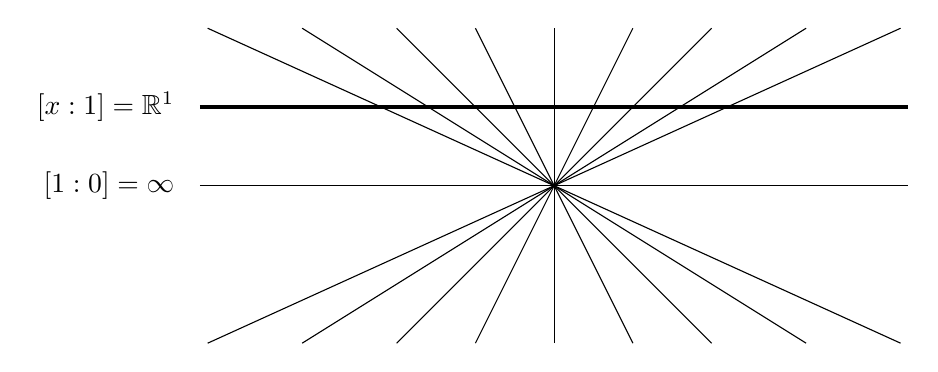
\begin{tikzpicture}
		\draw[very thick] (-4.5,1) -- (4.5,1) ;
		\draw (-4.5,0) -- (4.5,0) ;
		\draw (0,-2) -- (0,2);
		\draw (-2,-2) -- (2,2);
		\draw (-3.2,-2) -- (3.2,2);
		\draw (-1,-2) -- (1,2);
		\draw (2,-2) -- (-2,2);
		\draw (3.2,-2) -- (-3.2,2);
		\draw (1,-2) -- (-1,2);
		\draw (4.4,2) -- (-4.4,-2);
		\draw (4.4,-2) -- (-4.4,2);
		\draw (-4.7,1) node[left] {$[x:1]=\mathbb{R}^1$};
		\draw (-4.7,0) node[left] {$[1:0]=\infty$};
	\end{tikzpicture}
\end{center}
By introduce the continuous mapping
\begin{align*}
	r:P^1(\mathbb{R}) & \longrightarrow\mathbb{R}^1\cup\{\infty\}, \\
	[x:y]             & \longmapsto \frac{x}{y},
\end{align*}
we can clearly see $P^1(\mathbb{R})\cong S^1$.
$P^1(\mathbb{R})$ can be constructed by identifying the antipodal points of $S^1$.
\begin{center}
	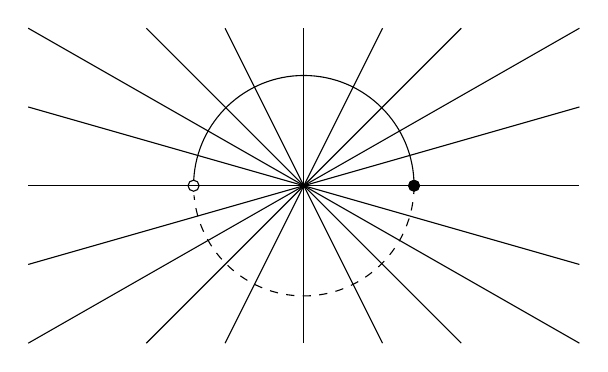
\begin{tikzpicture}
		\draw (1.4,0) arc [start angle=0, end angle=177, radius=1.4cm];
		\draw[dashed] (1.4,0) arc [start angle=0, end angle=-175, radius=1.4cm];
		\draw (-3.5,0) -- (3.5,0) ;
		\draw (0,-2) -- (0,2);
		\draw (-2,-2) -- (2,2);
		\draw (-3.5,-2) -- (3.5,2);
		\draw (-1,-2) -- (1,2);
		\draw (2,-2) -- (-2,2);
		\draw (3.5,-2) -- (-3.5,2);
		\draw (1,-2) -- (-1,2);
		\draw (3.5,1) -- (-3.5,-1);
		\draw (3.5,-1) -- (-3.5,1);
		\draw (-1.4,0) circle [radius=2pt];
		\filldraw (1.4,0) circle [radius=2pt];
	\end{tikzpicture}
\end{center}

\section{Two-dimensional manifolds: examples}
\subsection{Real affine plane $\mathbb{R}^2$}
The real affine plane $\mathbb{R}^2$ carries a standard topology. $\mathbb{R}^2$ is homeomorphic to any open region $G\in\mathbb{R}$.
Since the mapping $(x,y)\mapsto x+\mathrm{i}y$ is a homeomorphism, we have $\mathbb{R}^2\cong \mathbb{C}$.

\subsection{Sphere $S^2$}
The circle $S^2$ is defined by $S^2=\{(x,y,z)\in\mathbb{R}^3|x^2+y^2+z^2=1\}$. Similarly we have $S^2\cong \mathbb{R}^2\cup\{\infty\}$ and the stereographic projection of $P=(0,0,1)$
\begin{align*}
	pr:S^2-P\longrightarrow \mathbb{R}^2,\qquad      & (x, y,z) \longmapsto (X,Y)=\left(\frac{x}{1-z}, \frac{y}{1-z}\right),                                                             \\
	pr^{-1}:\mathbb{R}^1\longrightarrow S^1-P,\qquad & (X,Y) \longmapsto(x, y,z)=\left(\frac{2 X}{X^{2}+Y^{2}+1}, \frac{2 Y}{X^{2}+Y^{2}+1}, \frac{X^{2}+Y^{2}-1}{X^{2}+Y^{2}+1}\right).
\end{align*}
Sphere $S^2$ can be described by a square with some edges identified as follows
\begin{center}
	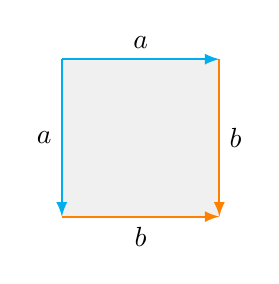
\begin{tikzpicture}
		\fill[fill=gray!12] (-1,-1) --(1,-1)--(1,1)--(-1,1)-- cycle;
		\draw [color=orange,thick,-latex] (-1,-1) -- node [color=black,pos=0.5,below]{$b$} (1,-1);
		\draw [color=cyan,thick,-latex] (-1,1) -- node [color=black,pos=0.5,left]{$a$} (-1,-1);
		\draw [color=orange,thick,-latex] (1,1)--node [color=black,pos=0.5,right]{$b$}(1,-1);
		\draw [color=cyan,thick,-latex] (-1,1)-- node [color=black,pos=0.5,above]{$a$} (1,1);
	\end{tikzpicture}
\end{center}

\subsection{Real projective plane $P^2(\mathbb{R})$}
Real projective plane $P^2(\mathbb{R})=(\mathbb{R}^3-\{(0,0,0)\})/\sim$ where $x\sim y$ whenever there is a nonzero real number $\lambda$ such that $x = \lambda y$. $P^2(\mathbb{R})\cong\mathbb{R}^2\sqcup P^1(\mathbb{R})\cong\mathbb{R}^2\sqcup\mathbb{R}^1\sqcup\{\infty\}$.
\begin{center}
	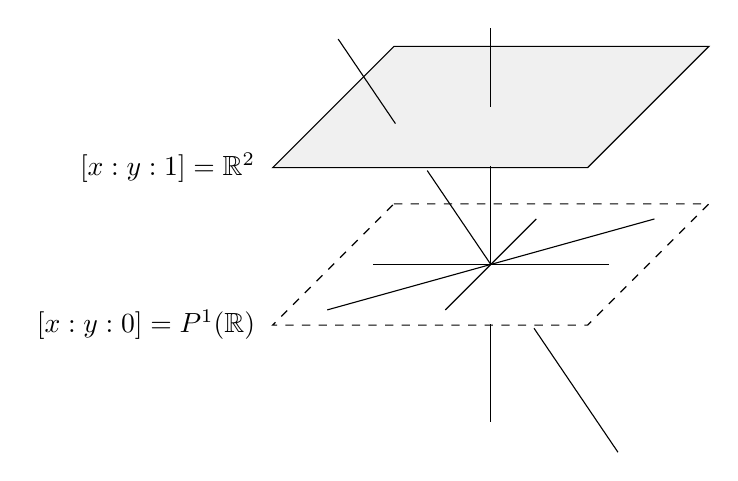
\begin{tikzpicture}
		\draw[dashed] (-2,0,-2) -- (2,0,-2)-- (2,0,2)-- (-2,0,2)--(-2,0,-2);
		\filldraw[fill=gray!12] (-2,2,-2) -- (2,2,-2)-- (2,2,2)-- (-2,2,2)--(-2,2,-2);
		\draw  (1.5,0,-1.5)-- (-1.5,0,1.5);
		\draw  (0,0,-1.5)-- (0,0,1.5);
		\draw  (1.5,0,0)-- (-1.5,0,0);
		\draw (0,-2,0) -- (0,-0.75,0);
		\draw (0,0,0) -- (0,1.25,0);
		\draw (0,2,0) -- (0,3,0);
		\draw (2,-2,1) -- (0.68,-0.68,0.34);
		\draw (0,0,0) -- (-1,1,-0.5);
		\draw (-1.5,1.5,-0.75) -- (-2.4,2.4,-1.2);
		\draw (-2.1,0,2) node[left]{$[x:y:0]=P^1(\mathbb{R})$};
		\draw (-2.1,2,2) node[left]{$[x:y:1]=\mathbb{R}^2$};
	\end{tikzpicture}
\end{center}
$P^2(\mathbb{R})$ can be constructed by identifying the antipodal points of $S^2$, which can be represented by $S^2/\{1,-1\}$. $P^2(\mathbb{R})$ can also be constructed from a closed unit disk $\overline{D^2}$ by identifying the antipodal points of the boundary $\partial \overline{D^2}=S^1$. Another way to describe $P^2(\mathbb{R})$ is a square with some edges identified as follows
\begin{center}
	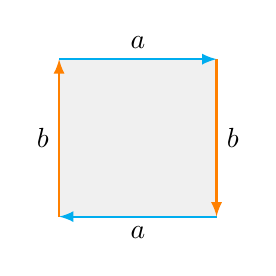
\begin{tikzpicture}
		\fill[fill=gray!12] (-1,-1) --(1,-1)--(1,1)--(-1,1)-- cycle;
		\draw [color=cyan,thick,-latex]  (1,-1)-- node [color=black,pos=0.5,below]{$a$} (-1,-1);
		\draw [color=orange,thick,-latex](-1,-1) -- node [color=black,pos=0.5,left]{$b$} (-1,1) ;
		\draw [color=orange,thick,-latex] (1,1)--node [color=black,pos=0.5,right]{$b$}(1,-1);
		\draw [color=cyan,thick,-latex] (-1,1)-- node [color=black,pos=0.5,above]{$a$} (1,1);
	\end{tikzpicture}
\end{center}
\subsection{Complex projective line $P^1(\mathbb{C})$}
Complex projective line $P^1(\mathbb{C})$ is the set of equivalence classes of $\mathbb{C}^2-{(0,0)}$ under the equivalence relation $\sim$ defined by $x\sim y$ if there is a nonzero complex number $\lambda$ such that $x = \lambda y$. We have the following homeomorphisms $P^1(\mathbb{C})\cong \mathbb{C}\cup\{\infty\}\cong \mathbb{R}^2\cup\{\infty\}\cong S^2$.
\subsection{Torus $T^2$}
A torus $T^2$ is a closed surface defined as the product of two circles $S^1 \times S^1$.
Torus can be described by a square with some edges identified as follows
\begin{center}
	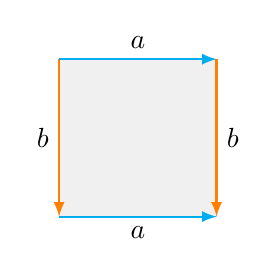
\begin{tikzpicture}
		\fill[fill=gray!12] (-1,-1) --(1,-1)--(1,1)--(-1,1)-- cycle;
		\draw [color=cyan,thick,-latex] (-1,-1) -- node [color=black,pos=0.5,below]{$a$} (1,-1);
		\draw [color=orange,thick,-latex] (-1,1)-- node [color=black,pos=0.5,left]{$b$}(-1,-1)  ;
		\draw [color=orange,thick,-latex] (1,1)--node [color=black,pos=0.5,right]{$b$}(1,-1);
		\draw [color=cyan,thick,-latex] (-1,1)-- node [color=black,pos=0.5,above]{$a$} (1,1);
	\end{tikzpicture}
\end{center}
\subsection{Möbius strip}
Möbius strip can be described by a square with some edges identified as follows
\begin{center}
	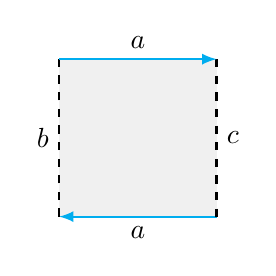
\begin{tikzpicture}
		\fill[fill=gray!12] (-1,-1) --(1,-1)--(1,1)--(-1,1)-- cycle;
		\draw [color=cyan,thick,-latex] (1,-1) -- node [color=black,pos=0.5,below]{$a$} (-1,-1);
		\draw [color=black,thick,dashed](-1,-1) -- node [color=black,pos=0.5,left]{$b$} (-1,1) ;
		\draw [color=black,thick,dashed] (1,1)--node [color=black,pos=0.5,right]{$c$}(1,-1);
		\draw [color=cyan,thick,-latex] (-1,1)-- node [color=black,pos=0.5,above]{$a$} (1,1);
	\end{tikzpicture}
\end{center}
\subsection{Klein bottle}

Klein bottle can be described by a square with some edges identified as follows
\begin{center}
	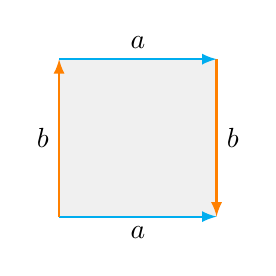
\begin{tikzpicture}
		\fill[fill=gray!12] (-1,-1) --(1,-1)--(1,1)--(-1,1)-- cycle;
		\draw [color=cyan,thick,-latex] (-1,-1) -- node [color=black,pos=0.5,below]{$a$} (1,-1);
		\draw [color=orange,thick,-latex](-1,-1) -- node [color=black,pos=0.5,left]{$b$} (-1,1) ;
		\draw [color=orange,thick,-latex] (1,1)--node [color=black,pos=0.5,right]{$b$}(1,-1);
		\draw [color=cyan,thick,-latex] (-1,1)-- node [color=black,pos=0.5,above]{$a$} (1,1);
	\end{tikzpicture}
\end{center}
\section{Compact two-dimensional manifolds: classification}
\subsection{Orientable surfaces}
Orientable surface of genus $g$ is a surface that has $g$ holes. It is denoted by $M_g$. For $g\ge 1$, $M_g$ can be described by a $4g$-gon with some edges identified as follows
\begin{center}
	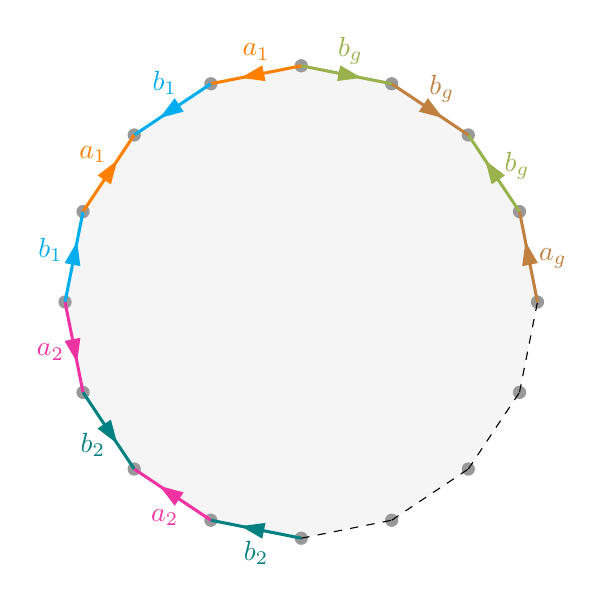
\begin{tikzpicture}
		\def\n{16} % Number of sides
		\def\radius{3cm} % Radius of the circumscribed circle
		\pgfmathsetmacro\startAngle{90} % Starting angle (top point)
	  
		% Define the vertices
		\foreach \i in {1,...,\n} {
		  \pgfmathsetmacro\angle{\startAngle + 360/\n * (\i - 1)}
		  \coordinate (V\i) at (\angle:\radius);
		}
		% Fill the interior region
		\fill[gray!8] (V1)
		\foreach \i in {2,...,\n} {
			-- (V\i)
		} -- cycle;
		\foreach \i in {1,...,\n} {
		  % Plot the vertices
		  \fill[black!40] (V\i) circle (2.4pt);
		}

		  % Draw the edges with arrowheads
		  \draw[->-, line width=1.1pt, color=orange] (V1) -- (V2) node[shift={(0, 0.05)}, midway, above] {$a_1$};
		  \draw[->-, line width=1.1pt, color=cyan] (V2) -- (V3) node[shift={(-0.1, 0.05)}, midway, above] {$b_1$};
		  \draw[-<-, line width=1.1pt, color=orange] (V3) -- (V4) node[shift={(-0.2, 0)}, midway, above] {$a_1$};
		  \draw[-<-, line width=1.1pt, color=cyan] (V4) -- (V5) node[shift={(-0.3, -0.2)}, midway, above] {$b_1$};
		  \draw[->-, line width=1.1pt, color=magenta!80] (V5) -- (V6) node[shift={(-0.3, -0.3)}, midway, above] {$a_2$};
		  \draw[->-, line width=1.1pt, color=teal] (V6) -- (V7) node[shift={(-0.2, 0.1)}, midway, below] {$b_2$};
		  \draw[-<-, line width=1.1pt, color=magenta!80] (V7) -- (V8) node[shift={(-0.1, -0.05)}, midway, below] {$a_2$};
		  \draw[-<-, line width=1.1pt, color=teal] (V8) -- (V9) node[shift={(0, -0.02)}, midway, below] {$b_2$};
		  \draw[dashed] (V9) -- (V10);
		  \draw[dashed] (V10) -- (V11);
		  \draw[dashed] (V11) -- (V12);
		  \draw[dashed] (V12) -- (V13);
		  \draw[->-, line width=1.1pt, color=brown] (V13) -- (V14) node[shift={(0, -0.02)}, midway, right] {$a_g$};
		  \draw[->-, line width=1.1pt, color=lime!40!gray] (V14) -- (V15) node[shift={(0, 0.1)}, midway, right] {$b_g$};
		  \draw[-<-, line width=1.1pt, color=brown] (V15) -- (V16) node[shift={(0.15, -0.05)}, midway, above] {$b_g$};
		  \draw[-<-, line width=1.1pt, color=lime!40!gray] (V16) -- (V1) node[shift={(0.05, 0)}, midway, above] {$b_g$};
	  \end{tikzpicture}
\end{center}
The fundamental group of $M_g$ is given by
\begin{equation*}
	\pi_1(M_g)=\langle a_1,b_1,\dots,a_g,b_g\mid [a_1,b_1]\dots[a_g,b_g]=1\rangle,
\end{equation*}
where $[a,b]=aba^{-1}b^{-1}$ is the commutator of $a$ and $b$. 

The cellular chain complex of $M_g$ is given by
\begin{equation*}
	0\longrightarrow \mathbb{Z} \overset{d_1}{\longrightarrow} \mathbb{Z}^{\oplus 2g}\overset{d_0}{\longrightarrow} \mathbb{Z}\longrightarrow 0,
\end{equation*}
\subsection{Non-orientable surfaces}
Non-orientable surface of genus $g$ is a surface that has  $g$ cross-caps attached to a sphere. It is denoted by $N_g$. For $g\ge 1$, $N_g$ can be described by a $2g$-gon with some edges identified as follows
\begin{center}
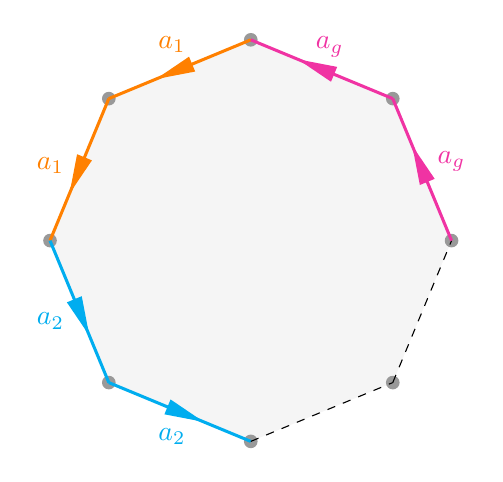
\begin{tikzpicture}[scale=0.85]
	\def\n{8} % Number of sides
	\def\radius{3cm} % Radius of the circumscribed circle
	\pgfmathsetmacro\startAngle{90} % Starting angle (top point)
  
	% Draw the vertices
	\foreach \i in {1,...,\n} {
	  \pgfmathsetmacro\angle{\startAngle + 360/\n * (\i - 1)}
	  \coordinate (V\i) at (\angle:\radius);
	}
	\fill[gray!8] (V1)
		\foreach \i in {2,...,\n} {
			-- (V\i)
		} -- cycle;
	\foreach \i in {1,...,\n} {
	  \fill[black!40] (V\i) circle (2.9pt);
	}
  
	% Draw the edges with arrowheads
	\draw[->-={5mm}, line width=1.1pt, color=orange] (V1) -- (V2) node[shift={(-0.1, 0.07)}, midway, above] {$a_1$};
	\draw[->-={5mm}, line width=1.1pt, color=orange] (V2) -- (V3) node[shift={(-0.06, 0.05)}, midway, left] {$a_1$};
	\draw[->-={5mm}, line width=1.1pt, color=cyan] (V3) -- (V4) node[shift={(-0.06, -0.12)}, midway, left] {$a_2$};
	\draw[->-={5mm}, line width=1.1pt, color=cyan] (V4) -- (V5) node[shift={(-0.1, -0.07)}, midway, below] {$a_2$};
	\draw[dashed] (V5) -- (V6);
	\draw[dashed] (V6) -- (V7);
	\draw[->-={5mm}, line width=1.1pt, color=magenta!80] (V7) -- (V8) node[shift={(0.06, 0.1)}, midway, right] {$a_g$};
	\draw[->-={5mm}, line width=1.1pt, color=magenta!80] (V8) -- (V1) node[shift={(0.1, 0.02)}, midway, above] {$a_g$};
  \end{tikzpicture}
\end{center}
\section{Other manifolds}
\subsection{Real projective space $P^n(\mathbb{R})$}
Real projective plane $P^n(\mathbb{R})=(\mathbb{R}^{n+1}-\{\mathbf{0}\})/\sim$ where $x\sim y$ whenever there is a nonzero real number $\lambda$ such that $x = \lambda y$. In general, we have
$$
	P^n(\mathbb{R})\cong S^n/\{\pm 1\}\cong D^n\sqcup (\partial D^n/{\pm 1})= D^n\sqcup (S^{n-1}/\{\pm 1\})\cong D^n\sqcup P^{n-1}(\mathbb{R})\cong \overline{D^n}\sqcup_{\partial D^n} P^{n-1}(\mathbb{R}),
$$
where $D^n:=\{x\in\mathbb{R}^{n+1}:\Vert x\Vert\le1\}$.

\chapter*{Appendix}

\begin{table}[h]
	\centering
	\begin{tblr}{
		colspec={|Q[m,c,1cm]|Q[m,c,1cm]|Q[m,c,1cm]|Q[m,c,0.8cm]|},
		row{1, 5} = {8ex},
		cell{1, 3, 5}{4} = {green7}}
		\hline
		\SetCell[r=5]{m} $\overline{A}$ & $A^\circ$                     & \SetCell[r=4]{m} $A'$ &\\ \cline{2-2} \cline{4-4}
		                                & \SetCell[r=4]{m} $\partial A$ &                       &\\ \cline{4-4}
		                                &                               &                       &\\ \cline{4-4}
		                                &                               &                       &\\ \cline{3-4}
		                                &                               & $A^s$                 &\\
		\hline
	\end{tblr}
\end{table}
\end{document}
